\documentclass[12pt,a4paper]{book}

\usepackage[utf8]{inputenc}
\usepackage[spanish]{babel}

\usepackage{amsmath}
\usepackage{amsfonts}
\usepackage{amssymb}
\usepackage{amsthm}
\usepackage{graphicx}
\usepackage[all]{xy}
\linespread{1}	% double spaces lines

\newcommand{\isEmbedded}{true}

\parindent 1.5pt
\parskip 5pt  % Also, a bit of space between paragraphs

\newtheorem{teo}{Teorema}[chapter]
\newtheorem{defi}[teo]{Definición}
\newtheorem{lem}[teo]{Lema}
\newtheorem{prop}[teo]{Proposición}
\newtheorem{cor}[teo]{Corolario}
\newtheorem{ej}{Ejercicio}

\def\K{\mathbb{K}}
\def\N{\mathbb{N}}
\def\C{\mathbb{C}}
\def\R{\mathbb{R}}
\def\Z{\mathbb{Z}}
\def\Q{\mathbb{Q}}
\def\P{\mathcal{P}}
\def\F{\mathcal{F}}
\def\c{\mathfrak{c}}
\def\si{\mathrm{\;si\:}}
\def\a0{\aleph_0}
\def\GL{\mathrm{GL}}
\def\Ort{\mathrm{O}}
\def\Uni{\mathrm{U}}
\def\Ima{\mbox{Im}}
\def\Id{\mbox{Id}}
\def\sep{\,\vert\,}
\newcommand{\cl}[1]{\overline{#1}}
\newcommand{\bb}[1]{\mathbb{#1}}
\newcommand{\inn}[1]{{{#1} \in \N}}
\newcommand{\ini}[1]{{{#1} \in I}}
\newcommand{\serie}[2]{\sum_{{#1} = 1}^{#2}}
\newcommand{\seriei}[1]{\sum_{{#1} = 1}^{\infty}}


\begin{document}
\begin{titlepage}
\begin{center}
\hrule 
{ \huge \bfseries Apunte Cálculo Avanzado}\\[0.4cm]
\hrule 
\Large
\emph{Autor:} Santiago Vega\\[0.4cm]
\emph{Versión} 2.0
\end{center}
\end{titlepage}

\thispagestyle{empty}
\vspace*{465pt}
Copyright \copyright  
2011-2012 Santiago Vega \\
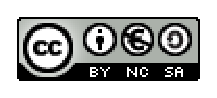
\includegraphics[scale=0.5]{cc.eps}\\
his work is licensed under the Creative 
Commons Attribution-NonCommercial-ShareAlike 3.0 Unported License. To
view a copy of this license, visit\\
 http://creativecommons.org/licenses/by-nc-sa/3.0/ or send a letter to
Creative Commons, 444 Castro Street, Suite 900, Mountain View, California, 94041, USA.

\chapter*{Introducción}
\thispagestyle{empty}
La idea de este apunte es sobretodo cubrir los temas de la materia Cálculo Avanzado de la carrera de Licenciatura en Ciencias Matemáticas de la Universidad De Buenos Aires. Bien puede ser utilizado por cualquier persona que busque una introducción a la teoría de espacios métricos, espacios normados y diferenciación en espacios de Banach. Contiene también un tratamiento en ligera profundidad de la teoría de cardinales, comenzando por un repaso básico de teoría de conjuntos. Decidí concretar esta presentación a la teoría de conjuntos desde el punto de vista ingenuo ya que requiere un tratamiento con menos delicadeza y profundidad que en su versión formal (léase Axiomas de Zermelo-Fraenkel), que no es el objetivo de este apunte, la sección de teoría de conjuntos está solo como un repaso y para marcar la notación del resto del apunte. \\
Originalmente este apunte fue concebido con tal de cubrir las faltas de bibliografía concreta en la parte de cardinalidad solamente y hacer unos comentarios abreviados sobre las otras secciones del programa de la materia, debido a la buena respuesta que obtuvo la primera versión, decidí tratar de completar y ampliar todos los temas de la materia.
\newpage
\thispagestyle{empty}
\setcounter{chapter}{0}
\pagenumbering{arabic}

\chapter{Cardinalidad}

\ifx\isEmbedded\undefined

\documentclass[12pt,a4paper]{book}

\usepackage[utf8]{inputenc}
\usepackage[spanish]{babel}

\usepackage{amsmath}
\usepackage{amsfonts}
\usepackage{amssymb}
\usepackage{amsthm}
\usepackage{graphicx}
\linespread{1}	% double spaces lines

\parindent 1.5pt
\parskip 5pt  % Also, a bit of space between paragraphs

\newtheorem{teo}{Teorema}[chapter]
\newtheorem{defi}[teo]{Definición}
\newtheorem{lem}[teo]{Lema}
\newtheorem{prop}[teo]{Proposición}
\newtheorem{cor}[teo]{Corolario}
\newtheorem{ej}{Ejercicio}

\def\K{\mathbb{K}}
\def\N{\mathbb{N}}
\def\C{\mathbb{C}}
\def\R{\mathbb{R}}
\def\Z{\mathbb{Z}}
\def\Q{\mathbb{Q}}
\def\P{\mathcal{P}}
\def\F{\mathcal{F}}
\def\c{\mathfrak{c}}
\def\si{\mathrm{\;si\:}}
\def\a0{\aleph_0}
\def\GL{\mathrm{GL}}
\def\Ort{\mathrm{O}}
\def\Uni{\mathrm{U}}
\def\Ima{\mbox{Im}}
\def\Id{\mbox{Id}}
\def\sep{\,\vert\,}
\newcommand{\cl}[1]{\overline{#1}}
\newcommand{\bb}[1]{\mathbb{#1}}
\newcommand{\inn}[1]{{{#1} \in \N}}
\newcommand{\ini}[1]{{{#1} \in I}}
\newcommand{\serie}[2]{\sum_{{#1} = 1}^{#2}}
\newcommand{\seriei}[1]{\sum_{{#1} = 1}^{\infty}}


\begin{document}
\else
\fi

\section{Teoría de conjuntos}
La teoría de conjuntos es fundacional para toda la matemática, es decir, desde el punto
de vista lógico, se puede deducir todo desde la teoría de conjuntos. Sin embargo aquí,
por falta de tiempo (y tal vez capacidad), nos limitamos a dar un repaso de ésta solo desde el punto de vista
ingenuo, que, como veremos más tarde, contiene contradicciones y problemas en las definiciones. Por ahora, aceptemos que los conjuntos existen y intentaremos dar una definición (algo intuitiva) de éstos: \\

\begin{defi} %Definicíon de conjunto
Un conjunto es una colección de objetos. $x \in A$ significa que $x$ pertenece a $A$.
\end{defi}

Aquí ya empezamos a ver que existen problemas, esta definición es vaga e imprecisa, pero esto es una de las delicadezas que no nos ocuparemos aquí, el lector debe confiar que todos estos conceptos pueden ser formalizados (de una u otra manera) de forma que no posean ninguna vaguedad. Sigamos con el resto de las proposiciones/definiciones que dan los objetos básicos con los que trabajaremos. El lector notará que si bien muchas llevan el nombre de ''Proposición'', éstas en realidad se asemejan más a definiciones y la razón que no llevan demostración alguna es que podria decirse que son claras en si mismas; no discutiremos la cuestiones lógicas de por qué son o no definiciones, proposiciones o bien axiomas. \newpage

\begin{prop} %Igualdad de conjuntos
Dos conjuntos son iguales si poseen los los mismos elementos \\
$$ A = B \Longleftrightarrow (x \in A \Leftrightarrow x\in B ) $$
\end{prop}

\begin{defi} %Definición de inclusión
Decimos que $A$ está incluido en $B$ o que $B$ contiene a $A$ si:
$$ \forall x \in A \Rightarrow x\in B $$
Es decir, que todos los elementos de $A$, también pertencen a $B$. Lo notamos como $ A \subseteq B $.
\end{defi}

\begin{ej} % Equivalencia entre doble inclusión y igualdad
Probar que $A \subseteq B$ y $A \supseteq B$, si y sólo si $A=B$
\end{ej}

\textbf{Notación:} Si $A \subseteq B$ y $A \neq B$ a veces escribimos $A \subset B$ ó $A \subsetneq B$ si queremos enfatizar el hecho que son distintos.

\begin{prop} % Existencia del vacío
Existe un conjunto sin elementos
$$ \exists A \slash \forall z , \, z \notin A $$ 
\end{prop}
\begin{ej}
Existe un único conjunto vacío. En base a esto, lo notamos como $\emptyset$.
\end{ej}
\begin{prop} % Existencia del conjunto con elementos dados
Para todo par $x,y$ de elementos, existe un conjunto cuyos elementos son $x$ e $y$.
$$ \forall x,y \, \exists z \slash t\in z \Leftrightarrow t=x \vee t=y$$
Notamos al conjunto $z$ como $ \lbrace x,y \rbrace $.
\end{prop}
La utilidad de esta ''proposición'', es la de crear conjuntos con elementos dados, de esta manera, considerando finitos elementos, siempre existe un conjunto que los contiene a todos ellos. \\[0.5cm]
Por cuestiones lógicas, no queda muy claro como definir un ''conjunto de conjuntos'', así, nos referimos en estos casos a una ''familia'' de conjuntos cuando queremos decir simplemente un ''grupo de conjuntos''. \\[0.5 cm]
Mostramos a continuación la existencia de la unión.

\begin{prop} %Unión
Dado un conjunto $A$ cuyos elementos son conjuntos, existe un conjunto $B$ que cumple que: \\
$$ B = \lbrace x \,\vert\, \exists z \in A \mbox{ que } x \in z \rbrace $$
Notamos a este conjunto $B$ como $\bigcup A$ y lo llamamos unión de los elementos de $A$.
\end{prop}

\textbf{Notación:} Si $A = \lbrace A_{j} \,\vert\, j \in J \rbrace$ notamos $\bigcup A$ como $\bigcup_{j\in J} A_{j}$.\\[0.5cm]
\textbf{Observación:} Es obvio que:
$$\bigcup \lbrace A \rbrace = A$$
\textbf{Notación:} Generalmente notamos $ \bigcup \lbrace A,B \rbrace$ como $A \cup B$, y esta suele ser la notación usual; en caso que se use ''$\bigcup$'' (a diferencia de ''$\cup$'') y ésta no lleve indices por debajo, nos referimos a la notación inicial, que para unir familias de conjuntos no indexados, resulta más cómoda.\\[0.5cm]
Ahora procedemos a mostrar la existencia de la intersección.

\begin{prop} %Intersección
Dado un conjunto $A$ cuyos elementos son conjuntos, existe un conjunto $B$ que cumple que:
$$ B = \lbrace x \,\vert\, \forall z \in A \mbox{ } x \in z \rbrace $$
Notamos a este conjunto $B$ como $\bigcap A$ y lo llamamos intersección de los elementos de $A$.
\end{prop}

\textbf{Notación:} Si $A = \lbrace A_{j} \,\vert\, j \in J \rbrace$ notamos $\bigcap A$ como $\bigcap_{j\in J} A_{j}$.\\[0.5cm]
\textbf{Observación:} Como antes, es obvio que
$$\bigcap \lbrace A \rbrace = A$$
\textbf{Notación:} Al igual que con la unión, generalmente notamos $ \bigcap \lbrace A,B \rbrace$ como $A \cap B.$, y usamos esta notación siempre, exceptuando en el caso que usemos ''$\bigcap$'' ésta y no lleve índices por debajo (a diferencia de ''$\cap$''), que como en la unión, nos referimos a la notación original.\\[0.5 cm]
\textbf{Observación:} Tanto la unión como la intersección pueden interpretarse como los conjuntos que cumplen propiedades características en cada caso:
\begin{itemize}
\item La unión de una familia de conjuntos es el conjunto más ''chico'' que contiene a todos. Y por más chico queremos decir que si $A$ representa la unión de todos y $B$ es otro conjunto que contiene a todos los conjuntos de la familia, resulta que $A \subseteq B$.
\item La intersección de una familia de conjuntos es el más ''grande'' que está contenido en todos. Por más grande queremos decir que si $A$ es la intersección de todos y $B$ es otro conjunto que está incluido en todos los conjuntos de la famila, resulta que $B \subseteq A$.
\end{itemize}

Dejamos ahora unas propiedades útiles como ejercicios sencillos.\newpage

\begin{ej} %Propiedades de unión y intersección.
Probar los siguientes enunciados:
\begin{enumerate}
\item $A \cup \emptyset = A$
\item $A \cup A = A $
\item $A \cup B = B \cup A$
\item $(A \cup B) \cup C = A \cup (B \cup C) $
\item $A \cap \emptyset = \emptyset$
\item $A \cap A = A $
\item $A \cap B = B \cap A$
\item $(A \cap B) \cap C = A \cap (B \cap C) $
\item $(A \cap B) \cup C = (A \cup C) \cap (B \cup C) $
\item $(A \cup B) \cap C = (A \cap C) \cup (B \cap C) $
\item $A \cap (\bigcup_{j \in J} B_{j}) = \bigcup_{j \in J} (B_{j} \cap A)$
\item $A \cup (\bigcap_{j \in J} B_{j}) = \bigcap_{j \in J} (B_{j} \cup A)$
\item $ A \cup B = B \Leftrightarrow A \subseteq B$
\item $ A \cap B = A \Leftrightarrow A \subseteq B$
\end{enumerate}
\end{ej}

\begin{defi} %Conjuntos disjuntos
Dados dos conjuntos $A$ y $B$ decimos que son disjuntos si $A \cap B = \emptyset$. Más generalmente, dada una familia de conjuntos $(A_i)_{i \in I}$, decimos que es disjunta dos a dos (a veces decimos simplemente disjunta) si $A_i \cap A_j = \emptyset$, para todo $i \neq j$
\end{defi}

\textbf{Notación:} Si tenemos dos conjuntos disjuntos $A,B$ y su correspondiente conjunto unión $A \cup B$, si queremos dar énfasis que su unión es entre dos conjuntos disjuntos, a veces lo notamos como $ A \sqcup B$. De manera análoga para simbolizar lo mismo para una familia de conjuntos disjuntos dos a dos notamos $ \bigcup_{i \in I} A_i$ como $\bigsqcup_{i \in I} A_i $. \\
Vale aclarar que esto es sólo una notación, es decir, si la familia original no es disjunta, indicar la unión con ''$\sqcup$'', no realiza la operación ''disjuntar la familia''; en tal circunstancia ésta notación está mal utilizada.\\[0.5 cm]
Mostraremos ahora qué es el conjunto de partes de un conjunto.

\begin{prop}[Partes de un conjunto]
Dado un conjunto $A$ existe un conjunto llamado partes de $A$ notado por $ \mathcal{P}(A)$ o también por $2^A$ que cumple:
$$ x \in \mathcal{P}(A) \Leftrightarrow x \subseteq A $$
Es decir, $\P(A)$ es el conjunto de todos los subconjuntos de $A$.
\end{prop}

Con esto definimos una partición de un conjunto, cosa que nos será útil luego.

\begin{defi} %Partición
Dado un conjunto $A$, definimos una partición de $A$ como cualquier subconjunto $P \subseteq \P(A)$ que cumpla:
\begin{itemize}
\item $ A = \bigcup P$
\item Si $X,Y \in P$ y $X \neq Y$, entonces $X \cap Y = \emptyset$
\end{itemize}
\end{defi}

\textbf{Ejemplos:}
\begin{itemize}
\item Dado $A$, el conjunto $\{A\}$ siempre es una partición. 
\item Dado el conjunto $\{ 1, 2, 3, 4\}$, una posible partición sería $\{\{1\},\{2,3\},\{4\}\}$.
\end{itemize}

\begin{defi} %Complemento
Dado un conjunto $\mathcal{U}$ definimos para todo conjunto $A \in \mathcal{P}(\mathcal{U})$ a $A^c$ (a veces también notado como $A'$) al conjunto que cumple que: $$ A^c = \lbrace x \in \mathcal{U} \,\vert\, x \notin A \rbrace $$
Llamamos a tal conjunto el complemento de $A$ en $ \mathcal{U}$. Es importante que la noción de complento tiene sentido sobre algún conjunto $\mathcal{U}$ y no de manera universal.
\end{defi}

\begin{ej} %Propiedades del complemento
Probar que dado $\mathcal{U}$ y $ A \in \mathcal{P}(\mathcal{U}) $ 
\begin{itemize}
\item $(A^c)^c = A $
\item $A \cap A^c = \emptyset $
\item $A \cup A^c = \mathcal{U}$
\item $\mathcal{U}^c = \emptyset$
\item $\emptyset^c = \mathcal{U}$
\end{itemize}
\end{ej}

\begin{defi} %Resta de conjuntos
Dados $A,B$ incluidos en un conjunto $\mathcal{U}$, definimos la resta de $A$ y $B$ como aquellos elementos de $A$ que no están en $B$:
$$ A \setminus B = A \cap B^c = \{ x \in A \,\vert\, x \notin B\}$$
\end{defi}

\begin{teo}[Leyes de De Morgan]
\hfill
\begin{itemize}
\item $(A \cup B )^c = A^c \cap B^c$
\item $(A \cap B )^c = A^c \cup B^c$
\end{itemize}
\begin{proof}
Demostraremos sólo el primer ítem, el otro es análogo. Para ver la igualdad veremos que ambos conjuntos se contienen mutuamente de acuerdo a la siguiente cadena de equivalencias:
\begin{align*}
x \in (A \cup B)^c &\Leftrightarrow x \notin A \cup B \\
\Leftrightarrow x \notin A \wedge x \notin B &\Leftrightarrow x \in A^c \cap B^c
\end{align*}
Por lo que (comprobando rápidamente las definiciones y proposiciones adecuadas) se obtiene la igualdad deseada.
\end{proof}
\end{teo}

Definiremos ahora los pares ordenados, que como el lector seguramente sabe, son increíblemente útiles e importantes para construir objetos en matemática, (como ser por ejemplo las relaciones y por lo tanto las funciones). Es considerada una las creaciones más importantes en la matemática, por más sencillo que el objeto pueda parecer.

\begin{defi} %Pares ordenados
Llamamos pares ordenados a los conjuntos de la forma $\lbrace \lbrace a \rbrace ; \lbrace a,b \rbrace \rbrace$, con $a$ y $b$ dos elementos cualesquiera, notamos a estos conjuntos como $(a,b)$.
\end{defi}

\begin{teo} %Igualdad de pares ordenados
$ (a,b) = (c,d) \Leftrightarrow (a = c \wedge b = d) $
\begin{proof}
$(\Rightarrow)$  Si $(a,b) = (c,d)$ por definición tenemos que:
$$ \{ \{ a \} ; \{ a,b \} \} = \{ \{ c \} ; \{ c,d \} \} $$
Por lo que como ésta es una igualdad entre conjuntos tenemos que, los elementos que estan incluidos deben ser los mismos.\\
\underline{Si $a=b$:} En este caso tenemos que $\lbrace a \rbrace = \lbrace a,b \rbrace$ \\
Como la cantidad de elementos de dos conjuntos iguales es la misma debe ser que: 
$$ \{ a \} = \{ c \} = \{ a,b \} = \{ c,d \}$$
Así se ve que $ a = c = b = d $ \\
\underline{Si $a\neq b$:} Suponiendo que $ c \neq d$ se llega a que $\lbrace a \rbrace = \lbrace c \rbrace$ por lo que $ a = c$ rápidamente se ve que $b = d$.\\
Si $c = d$ se ve que debe pasar que son todos iguales (reduciéndolo al caso anterior), lo cual es absurdo ya que dijimos que $ a \neq b $ \\
$(\Leftarrow)$ Es claro ya que son los mismos conjuntos.
\end{proof}
\end{teo}
 
Ahora definiremos qué es el producto cartesiano en el caso finito

\begin{defi} %Producto cartesiano finito
Llamamos producto cartesiano de dos conjuntos $A$ y $B$ al conjunto:
$$ A\times B := \lbrace (a,b) \,\vert\, a \in A \mbox{ y } b \in B \} $$
En caso de tener conjuntos $A_1, \ldots , A_k$, podemos definir:
$$ A_1 \times \ldots \times A_k = A_1 \times ( A_2 \times ( \ldots \, A_k) \ldots )$$
Y para simplificar la notación, podemos notar los elementos de $ A_1 \times \ldots \times A_k$ como $(a_1, \ldots,a_k)$, donde cada $a_i \in A_i$, obviando paréntesis inecesarios.
\end{defi}

\textbf{Notación:} En general escibimos $A^n = \underbrace{A \times \ldots \times A}_ {n \; veces}$.\\[0.5cm]
Más adelante generalizaremos la noción de producto cartesiano a infinitos conjuntos.\\[0.5cm]
Por último, para cerrar esta sección comentaremos porque esta teoría de conjuntos ingenua no es correcta y cual es uno de sus más importantes problemas. Todo se debe a que la concepción de conjunto que posee esta concepción de la teoría, es una idea intuitiva y muy blanda que puede ser manipulada para poder lograr resultados paradójicos. El más común de estos ejemplos es el de la Paradoja de Russell ideada por Bertrand Russell (1872 - 1970), aunque la idea escencial de su construcción remite a la antigua Grecia (Paradoja de Epiménides).\\

\textbf{Paradoja de Russell:} Sea $A = \{ a \,\vert\, a \notin a\}$.\\ Entonces nos preguntamos ¿$A \in A$ ó $A \notin A$?\\Si $ A \in A $ entonces $A \notin A$, lo que es absurdo; pero si $ A \notin A $ entonces $A \in A$ otra vez absurdo. ¡Lo cual es una contradicción, ya que el conjunto $A$ es un conjunto totalmente válido! ¿O no?\\
La respuesta corta es que no, no es un conjunto, pero la respuesta larga es un poco más complicada que eso:\\
La solución que encontraron los matemáticos de la época (principios del siglo XX) para resolver la Paradoja de Russell (y otras más) fue dar un sistema formal donde la contrucción de la paradoja (y otras paradojas más) carecieran de sentido y no puediesen establecerse estas contradicciones, así de alguna manera retirando el estatus de conjunto al ''conjunto'' $A$ antes definido y concretando la teoría moderna de conjuntos. El sistema formal que se considera más estándar hoy en día es el formulado por Ernst Zermelo (1871 - 1953) y Abraham Fraenkel (1891 - 1965) así llamado teoría de conjuntos de Zermelo-Fraenkel (abreviada ZF); aún así, existen otras teorías formuladas por Kurt Gödel (1906 - 1978), John Von Neumann (1903 - 1957) y muchos otros. A pesar de que ZF es la más aceptada aún no se sabe si posee contradicciones, es decir, si es consistente. Este proceso motivó fuertemente la filosofía de la matemática moderna motivando resultados muy profundos en lógica (como los teoremas de incompletidtud de Gödel).

\ifx\isEmbedded\undefined
\end{document}
\else
\fi
\newpage
\ifx\isEmbedded\undefined

\documentclass[12pt,a4paper]{book}

\usepackage[utf8]{inputenc}
\usepackage[spanish]{babel}

\usepackage{amsmath}
\usepackage{amsfonts}
\usepackage{amssymb}
\usepackage{amsthm}
\usepackage{graphicx}
\linespread{1}	% double spaces lines

\parindent 1.5pt
\parskip 5pt  % Also, a bit of space between paragraphs

\newtheorem{teo}{Teorema}[chapter]
\newtheorem{defi}[teo]{Definición}
\newtheorem{lem}[teo]{Lema}
\newtheorem{prop}[teo]{Proposición}
\newtheorem{cor}[teo]{Corolario}
\newtheorem{ej}{Ejercicio}

\def\K{\mathbb{K}}
\def\N{\mathbb{N}}
\def\C{\mathbb{C}}
\def\R{\mathbb{R}}
\def\Z{\mathbb{Z}}
\def\Q{\mathbb{Q}}
\def\P{\mathcal{P}}
\def\F{\mathcal{F}}
\def\c{\mathfrak{c}}
\def\si{\mathrm{\;si\:}}
\def\a0{\aleph_0}
\def\GL{\mathrm{GL}}
\def\Ort{\mathrm{O}}
\def\Uni{\mathrm{U}}
\def\Ima{\mbox{Im}}
\def\Id{\mbox{Id}}
\def\sep{\,\vert\,}
\newcommand{\cl}[1]{\overline{#1}}
\newcommand{\bb}[1]{\mathbb{#1}}
\newcommand{\inn}[1]{{{#1} \in \N}}
\newcommand{\ini}[1]{{{#1} \in I}}
\newcommand{\serie}[2]{\sum_{{#1} = 1}^{#2}}
\newcommand{\seriei}[1]{\sum_{{#1} = 1}^{\infty}}


\begin{document}
\else
\fi

\section{Relaciones, órdenes y funciones}
Repasaremos los resultados de relaciones ya que serán necesarios para la sección siguiente, estableciendo resultados acerca del axioma de elección y sus equivalencias.

\begin{defi} %Definición de relación
Una relación de $A$ en $B$ es un subconjunto de $A \times B$
\end{defi}

\begin{defi} %Definición de función
Una función de $A$ en $B$ es una relación $f$ de $A$ en $B$ que cumple que:
$$ \forall a \in A \mbox{ , } \exists ! b \in B \mbox{ tal que } (a,b) \in f$$
Es decir, $f$ es una función si todos los elementos de $A$ estan relacionados con un único elemento en $B$ vía $f$. Al conjunto $A$ se lo llama dominio de $f$ y al conjunto $B$ codominio de $f$. Notamos a una función $f$ de $A$ en $B$ como $f:A \rightarrow B$.
\end{defi}

\textbf{Notación:} Si el par $(a,b)$ pertenece a la función $f$, escribimos $f(a)=b$. En algunas oportunidades, por comodidad, utilizaremos el hecho de que una función es un conjunto de pares, pero en general no lo utilizaremos nunca.\\[0.5cm]
Asociamos la idea de igualdad de funciones a que tienen exactamente los mismos pares que las forman:
\begin{defi} Dadas dos funciones $f,g:A \rightarrow B$ decimos que $f = g$ si y sólo si $f(x) = g(x)$ para todo $x \in A$.
\end{defi}
El lector puede corroborar que esta idea es la misma que decir que $f=g$ como conjuntos de pares\\[0.5cm]
Damos la notacion útil de restricción y corestricción que utilizaremos para funciones:\\
\textbf{Notación:} Dada una función $f:A \rightarrow B$, y subconjuntos $C \subseteq A$ y $D \subseteq B$, cuando hacemos referencia a la función que vale lo mismo que $f$ pero con dominio $C$ escribimos $f \vert_C$ y la llamamos restricción de $f$ a $C$, esto podemos realizarlo para cualquier función y obviamente tenemos que $f \vert_C : C \rightarrow B$ y $f \vert_C (x) = f(x)$ para todo $x \in C$. De la misma manera podemos plantearnos la noción de correstricción donde la función correstringida es escencialmente igual que la función original pero con un codominio más chico, escribimos en este caso $f \vert^D$ y tenemos que $f \vert^D :A \rightarrow D$ y $f \vert^D(x) = f(x)$. Para que la correstricción esté bien definida, debe suceder que $f(x) \in D$ para todo $x$ en el dominio, de lo contrario no tendría sentido.\\
Si queremos combinar las dos nociones escribimos $f \vert_C^D := f \vert_C \vert^D : C \rightarrow D$.\\[0.5cm]
\textbf{Notación} A la función de un conjunto $X$ en si mismo que manda cada elemento en si mismo la llamamos función identidad, la notamos por $\Id_X : X \rightarrow X$ y $\Id_X(x)=x$. Cuando el conjunto $X$ en cuestión está claro del contexto notamos simplemente $\Id$.
Definimos composición de funciones:
\begin{defi} Dadas funciones $f:A \rightarrow B$ y $g: B \rightarrow C$, definimos la composición $g \circ f:A \rightarrow C$ como $g\circ f(x) = g(f(x))$
\end{defi}
\textbf{Notación:} A veces para definir una función $f:A \rightarrow B$ escribimos:
\begin{align*}
A &\overset{f}{\longrightarrow} B \\
a &\longmapsto f(a)
\end{align*}
Donde ''$\mapsto$'' simboliza ''a través de $f$ va a parar en''. Si no requerimos darle un nombre a la función a veces no escribimos la ''$f$'' sobre la flecha superior.\\[0.5cm]
Definimos ahora la imagen de una función.
\begin{defi} Si $f: A \rightarrow B$ es una función definimos la imagen de $f$ como el conjunto
$$ \Ima(f)=\{ f(x) \,\vert\, x \in A\} \subseteq B$$
En general, dado un subconjunto $C\subseteq A$ definimos $f(C) = \{ f(x) \,\vert\, x \in C\}$, de esta manera $\Ima(f) = f(A)$.
\end{defi}
Análogamente definimos la preimagen de un conjunto
\begin{defi}Si $f: A \rightarrow B$ es una función y $C \subset B$ definimos la preimagen de $C$ vía $f$ como el conjunto:
$$ f^{-1}(C) = \{  x \in A \,\vert\, f(x) \in C\}$$
\end{defi}
\textbf{Notación:} Si queremos hacer referencia a todas las funciones de $A$ en $B$ escribimos:
$$ B^A = \{ f \,\vert\, f:A \rightarrow B\}$$
Damos ahora algunas definiciones acerca de propiedades de funciones:
\begin{defi}
Dada una función $f:A \rightarrow B$ decimos que:
\begin{itemize}
\item $f$ es inyectiva si sucede que $f(x) = f(y)$ si y sólo si $x = y$.
\item $f$ es suryectiva (o a veces sobreyectiva) si dado un elemento $y \in B$, existe $x \in A$ tal que $f(x)=y$.
\item $f$ es biyectiva si es inyectiva y sobreyectiva
\end{itemize}
\end{defi}
\begin{ej} Dada una función $f:A \rightarrow B$ probar que
\begin{itemize}
\item $f$ es sobreyectiva si y sólo si $\Ima(f)=B$
\item $f\vert^{\Ima(f)}$ es sobreyectiva.
\item Si $Y\subseteq X$ la función, $i:Y \rightarrow X$ dada por $i(y)=y$ es inyectiva. Llamamos a esta función, la función inclusión de $Y$ en $X$.
\item Si $f$ es biyectiva existe una única función $g$ tal que $g \circ f = \Id_A$ y $f \circ g = \Id_B$. Notamos a $g$ como $f^{-1}$. No confundir con la notación de preimagen, aunque, sugestivamente, cuando la función es biyectiva ambos conjuntos coinciden.
\item Si $f$ es inyectiva, entonces existe una función $g:B \rightarrow A$ (no necesariamente única) tal que $g \circ f = Id_A$. Llamamos a esta $g$ la inversa a izquierda de $f$.
\end{itemize} 
\end{ej}
Ahora que tenemos elementos teóricos acerca de funciones podemos dar la generalización de un producto cartesiano:
\begin{defi} %Producto cartesiano general
Dada una familia de conjuntos $ A_j : j \in J $ (no necesariamente finita) definimos el producto cartesiano como:
$$ \prod_{j \in J} A_j = \lbrace f: J \rightarrow \bigcup_{j \in J} A_j \,\vert\, f(j) \in A_j \forall j\in J \} $$
\end{defi}

\textbf{Observación:} ¿Por qué definimos el caso finito e infinito de manera diferente? En primer lugar veamos que en el caso finito ambas definiciones son consistentes: Dados $A_1 , \ldots , A_k$ y su producto cartesiano como en la primera definición, tomando un elemento de la forma $(a_1, \ldots,a_k)$ podemos crear una función que cumpla con los requerimientos de la segunda definición donde $ J = \{1 , \ldots , k\}$ y $f(i)=a_i$, además es claro que de esta manera la función que toma estos valores es única; de manera recíproca, dada una función $g$ que cumpla la segunda definición, se representa como la upla $(g(1), \ldots , g(k))$, por lo que vemos que escencialmente ambas definiciones dan el mismo resultado.\\
Ahora, la razón de porqué en el caso general se define de esta manera es debido a que en algunos casos dar una ''upla'' infinita no queda exactamente claro y es más engorroso de definir concretamente, esto se debe a cuestiones con la cardinalidad de la familia de conjuntos (que abordaremos en esa sección de este capítulo); usando la segunda definición, el producto queda definido de una manera concisa y clara y después se utiliza por lo general la notación en ''uplas infinitas'' para representar las funciones.\\Otra observación pertinente es que, a priori, en un producto cartesiano arbitrario (bajo la segunda definición), nadie nos garantiza que exista una función que cumpla esas propiedades; sabemos que en el caso finito existe (construyéndola por inducción) pero no lo sabemos en otros casos. \\[0.5cm]	
Asociado al concepto de producto cartesiano, viene la idea de proyección, que es muy útil y de suma importancia ya que se puede demostrar (no lo haremos aquí) que caracteriza al producto cartesiano (en el sentido de que si hay otro conjunto, con un juego de funciones que actúan como proyecciones, entonces hay una única función biyectiva entre ese conjunto y el producto cartesiano, a esta propiedad se la llama Propiedad Universal del Producto Cartesiano).
\begin{defi}
Si $\{A_i \,\vert\, i \in I\}$ es una familia de conjuntos (finita o infinita) y $A = \prod_{i \in I} A_i$ es su producto cartesiano, llamamos a la proyección $i$-ésima a la función $\pi_i:A \rightarrow A_i$ dada por:
$$ \pi_i(f) = f(i)$$
Sino también considerando a los elementos de $A$ como uplas: 
$$ \pi_i((x_i)_{i\in I}) = x_i$$
\end{defi}

Veamos algunas clasificaciones de propiedades de relaciones:
\begin{defi} % Reflexividad, simetría, ...
Dada una relación $\mathcal{R} \subseteq A \times A$, se dice que una relación es:
\begin{enumerate}
\item Reflexiva si para cualquier $a \in A$, siempre $(a,a) \in \mathcal{R}$.
\item Simétrica si dado un par $(a,b)\in \mathcal{R}$ entonces también $(b,a) \in \mathcal{R}$
\item Antisimétrica si dados los pares $(a,b),(b,a)\in \mathcal{R}$ resulta que $a = b$
\item Transitiva si dados los pares $(a,b),(b,c) \in \mathcal{R}$, tenemos que $(a,c) \in \mathcal{R}$
\end{enumerate}
\end{defi}

Ahora usaremos estas propiedades para dar ciertos tipos de relaciones que poseen propiedades útiles e importantes.

\begin{defi}(Tipos de relaciones)
Una relación $\mathcal{R} \subseteq A \times A$ se dice:
\begin{itemize}
\item De equivalencia si es reflexiva, simétrica y transitiva.
\item Un preorden si es reflexiva y transitiva.
\item Un orden si es un preorden y es antisimétrica.
\end{itemize}
\end{defi}

No haremos mucho enfasis en el uso general de las relaciones, nos centraremos en el uso de las relaciones de orden que nos serán utiles para manipular la teoría detras de las equivalencias del Axioma de Elección en la sección siguiente y resultados acerca de cardinalidad. Por lo que, como no las expondremos aquí porque no las utilizaremos, vale aclarar que las relaciones de equivalencia poseen muchas propiedades interesantes como por ejemplo, la de caracterizar una partición del conjunto.

\textbf{Notación:} Si $\mathcal{R}$ es una relación, en ciertas ocaciones escribimos $a \mathcal{R} b$ en vez de $(a,b) \in \mathcal{R}$.\\[0.5cm]
Desde ahora, nos concentraremos en propiedades de conjuntos ordenados, que pasamos a definir.

\begin{defi} %Def de poset
Si $A$ es un conjunto con un orden $\leq$, denominamos al par $(A,\leq)$ como un poset (del inglés ''partially ordered set'').
\end{defi}

Algunos nombres útiles.

\begin{defi} % Mínimo, máximo, etc
Sea $(A,\leq)$ un poset. Dado $ X \subseteq A$ definimos:
\begin{itemize}
\item Un elemento $x \in X$ es máximo si para todo $y \in X $ sucede que $ y \leq x$.
\item Un elemento $x \in X$ es mínimo si para todo $y \in X $ sucede que $ x \leq y$.
\item Un elemento $x \in X$ es maximal si dado un $ y \in X $ tal que $ x \leq y$, entonces $ x = y$.
\item Un elemento $x \in X$ es minimal si dado un $ y \in X $ tal que $ y \leq x$, entonces $ x = y$.
\item Un elemento $a \in A$ es una cota superior de $X$ si $x \leq a$ , para todo $x \in X$.
\item Un elemento $a \in A$ es una cota inferior de $X$ si $a \leq x$ , para todo $x \in X$.
\end{itemize}
\end{defi}

\begin{defi} %Totalmente ordenado
Un poset $(A,\leq)$ se dice totalmente ordenado si para todo $a,b \in A$ sucede que $a \leq b$ ó $b \leq a$.
\end{defi}

\begin{defi} %Cadena
Una cadena de un poset $(A,\leq)$ es un subconjunto de $A$ que con el orden $\leq$ es totalmente ordenado.
\end{defi}

\begin{defi} %Bien ordenado
Un poset $(A,\leq)$ es bien ordenado si para todo $B \in \mathcal{P}(A)$, suecede que $B$ posee mínimo (con el orden restringido).
\end{defi}

\textbf{Notación:} Generalmente notamos a una relacion de orden como $\leq$ o en algunas ocasiones como $\unlhd$. Cuando queremos decir que $x \leq y$ y además $x \neq y$, muchas veces escribimos $x < y$ o a veces $x \lneq y$, de la misma manera si queremos decir $x \unlhd y$ y $x \neq y$ escribimos $x \lhd y$.

Una proposición importante:
\begin{prop} % Bien ord implica totalmente ord
Todo conjunto bien ordenado es totalmente ordenado.
\begin{proof}
Sea $(A,\leq)$ un conjunto bien ordenado, entonces o bien $A$ posee un único elemento (en el cual, es claro que es un conjunto totalmente ordenado) o tiene por lo menos dos elementos. Si es este el caso, sean $a,b \in A$. Entonces $\{ a,b \} \in \mathcal{P}(A)$, por lo que, como $A$ es bien ordenado, este conjunto posee mínimo, entonces debe suceder que $a \leq b$ o $b \leq a$.
\end{proof}
\end{prop}
Algunos ejercicios sencillos:
\begin{ej} Dado un poset $(X,\leq)$
\begin{itemize}
\item Todo subconjunto de una cadena es una cadena.
\item Todo subconjunto de un conjunto bien ordenado está bien ordenado.
\end{itemize}
\end{ej}
\textbf{ Ejemplos:} 
\begin{itemize}
\item El ejemplo canónico de conjunto bien ordenado es $ \mathbb{N}$ que puede demostrarse fácilmente usando inducción.
\item Ejemplos de conjuntos totalmente ordenados: $\N$, $\Z$, $\Q$ ,$\R$.
\item El conjunto de partes de un conjunto arbirtario, junto con la relación de inclusión es un conjunto ordenado, no total.
\item Un conjunto totalmente ordenado no es necesariamente bien ordenado, mostrando que la reciproca de la proposición anterior es falsa: En $\R$ el conjunto $\{ x \in \R \,\vert\,  0 < x \} = (0;+\infty)$ no posee mínimo, ya que dado un número real positivo $x$, $\frac{x}{2}$ es menor estricto que $x$ y positivo. Sin embargo $\R$ posee conjuntos bien ordenados ($\N \subseteq \R$).
\end{itemize}
 
\ifx\isEmbedded\undefined
\end{document}
\else
\fi

\newpage
\ifx\isEmbedded\undefined

\documentclass[12pt,a4paper]{book}

\usepackage[utf8]{inputenc}
\usepackage[spanish]{babel}

\usepackage{amsmath}
\usepackage{amsfonts}
\usepackage{amssymb}
\usepackage{amsthm}
\usepackage{graphicx}
\linespread{1}	% double spaces lines

\parindent 1.5pt
\parskip 5pt  % Also, a bit of space between paragraphs

\newtheorem{teo}{Teorema}[chapter]
\newtheorem{defi}[teo]{Definición}
\newtheorem{lem}[teo]{Lema}
\newtheorem{prop}[teo]{Proposición}
\newtheorem{cor}[teo]{Corolario}
\newtheorem{ej}{Ejercicio}

\def\K{\mathbb{K}}
\def\N{\mathbb{N}}
\def\C{\mathbb{C}}
\def\R{\mathbb{R}}
\def\Z{\mathbb{Z}}
\def\Q{\mathbb{Q}}
\def\P{\mathcal{P}}
\def\F{\mathcal{F}}
\def\c{\mathfrak{c}}
\def\si{\mathrm{\;si\:}}
\def\a0{\aleph_0}
\def\GL{\mathrm{GL}}
\def\Ort{\mathrm{O}}
\def\Uni{\mathrm{U}}
\def\Ima{\mbox{Im}}
\def\Id{\mbox{Id}}
\def\sep{\,\vert\,}
\newcommand{\cl}[1]{\overline{#1}}
\newcommand{\bb}[1]{\mathbb{#1}}
\newcommand{\inn}[1]{{{#1} \in \N}}
\newcommand{\ini}[1]{{{#1} \in I}}
\newcommand{\serie}[2]{\sum_{{#1} = 1}^{#2}}
\newcommand{\seriei}[1]{\sum_{{#1} = 1}^{\infty}}


\begin{document}
\else
\fi

\section{El Axioma de elección y sus equivalencias}

Aquí mostramos que es el axioma de elección y ,más importante aún, cuales son sus equivalencias lógicas. Como afimamos antes, la teoría de conjuntos que presentamos en este apunte es inconsistente, pero aclararemos que dentro de la teoría de conjuntos de Zermelo-Fraenkel, la gran mayoría de los conceptos usados aquí son similares en interpretación.\\
Definiremos antes que nada qué es una función elección:

\begin{defi} %Función elección
Una función elección de una familia de conjuntos no vacíos $\{A_j \,\vert\, j \in J\}$, es una función de $\{A_j\}_{j \in J}$ en $ \bigcup_{j \in J} A_j $ que cumple que para todo $A_j$, $f(A_j) \in A_j$. Es decir una función que asigna un elemento de si mismo a cada conjunto $A_j$ (de ahí que se llame ''de elección'' o ''selectora'').
\end{defi}

Ahora expresaremos la formulación usual del axioma de elección\\[0.5cm]
\textbf{Axioma de Elección:} Toda familia de conjuntos no vacíos posee una función elección. (abreviado AC, del inglés, ''Axiom of Choice'') \\[0.5cm]
Precisamente porque la noción intuitiva de este postulado resulta razonable, se lo considera un axioma (es decir, verdadero porque sí). Su mayor importancia radica en los resultados importantes que puede producir y si lo queremos como cierto. debe asumirse como axioma, ya no puede ser deducido lógicamente de los Axiomas de Zermelo-Fraenkel (abreviado ZF), suponiendo que estos son consistentes (libres de contradicciones). Como veremos a continuación, los resultados que produce este axioma producen que se cuestione que tan ''razonable'' es.\\
La principal razón de por qué no puede deducirse del sistema ZF, es que en el caso de que la familia de conjuntos sea infinita, como los elementos elegidos son ''al azar'', se necesitaría una infinita cantidad de pasos para construir tal función, por lo que la demostración de tal ''teorema'' tendría longitud infinita y obviamente no se admiten demostraciones tales. Si los elementos pudiesen ser elegidos en base a un algoritmo, entonces no habría problema. En definitva, es una herramienta muy útil para afirmar existencia de ciertos tipos de elementos, cuando estos son incostructibles desde el punto de vista algorítmico.\\[0.5cm]
Veamos otras formulaciones de AC\newpage
\textbf{ACII:} Dado un conjunto $A \neq \emptyset$, existe una función elección de la familia $\P(A) \setminus \{\emptyset\}$.\\[0.5cm]
\textbf{ACIII:} Dada una familia de conjuntos no vacíos $\{A_j \,\vert\, j \in J\}$ el producto cartesiano cumple que
$$ \prod_{j \in J} A_j \neq \emptyset$$\\
Y ahora veamos su equivalencia:

\begin{prop} %Equivalencia de las caracterizaciones de AC
AC, ACII y ACIII, son equivalentes (en el marco de ZF)
\begin{proof}
(AC $\Rightarrow$ ACII) Si AC es cierto, y $A\neq \emptyset$ entonces $\P(A) \setminus \{\emptyset\}$ es una familia conjuntos no vacía, por lo que ésta posee función elección y así ACII es cierto.\\
(ACII $\Rightarrow$ ACIII) Dada la familia $\{A_j : j \in J\}$ de conjuntos no vacíos y consideramos $\mathcal{A}$, su unión, ésta es no vacía, por lo que existe, según ACII, una función elección $f$ de $\P(\mathcal{A}) \setminus \{\emptyset\}$, en particular, como cada $A_j \in \P(\mathcal{A}) \setminus \{\emptyset\}$, tenemos que $f(A_j) \in A_j$ por ser ésta una función elección, pero entonces $f \in \prod_{j \in J} A_j$, lo que muestra que $\prod_{j \in J} A_j$ es no vacío.
(ACIII $\Rightarrow$ AC) Dada una familia $\{A_j : j \in J\}$ de conjuntos no vacíos y tomamos $f \in \prod_{j \in J} A_j$ (que es no vacío por hipotesis), entonces $f(A_j) \in A_j$ por lo que $f$ es una función elección.
\end{proof}
\end{prop}
Dejamos dos ejercicios útiles:
\begin{ej} Asumiendo que AC (o cualquiera de sus equivalencias antes vistas) demostrar que dada una función $f: A \rightarrow B$ sobreyectiva, existe una función $g:B \rightarrow A$ (no necesariamente única) tal que $f \circ g = Id_B$. Llamamos a $g$ la inversa a derecha de $f$.
\end{ej}
\begin{ej}
Demostrar que si asumimos como cierto el hecho de que toda función sobreyectiva admite una inversa a derecha entonces AC debe ser cierto.
\end{ej}
Veamos otros postulados: \\[0.5cm]
\textbf{Axioma (Principio de Buena Ordenación):} Dado un conjunto $A$ no vacío, existe una relación de orden $\leq$, tal que $(A,\leq)$ es un poset bien ordenado. (Abreviado WOP del inglés ''Well-Ordering Principle'')\\[0.5cm]
\textbf{Axioma (Principio Maximal de Hausdorff):} Dado un poset $(A,\leq)$ no vacío, existen cadenas que son maximales en el sentido de la inclusión, es decir, existe una cadena $L$, tal que si existe otra cadena $S \supseteq L$, entonces $S = L$. (Abreviado HMP del inglés ''Hausdorff Maximal Principle'', debido al matemático Felix Hausdorff (1868 - 1942))\\[0.5cm]
\textbf{ Axioma (Lema de Zorn):} Dado un poset $(A,\leq)$, no vacío, que cumple que para toda cadena $L \subseteq A$, ésta posee máximo, entonces $A$ posee al menos un elemento maximal. (abreviado ZL del inglés ''Zorn's Lemma'', debido al matemático Max Zorn (1906 - 1993)) \\[0.5cm]
Analicemos un poco estos axiomas. El más ''controversial'' por así llamarlo, es WOP, esto se debe a que hay conjuntos (como $\R$) que son dificiles de imaginar que posean un buen orden. Tanto HMP como ZL son má complejos de comprender su verdadera escencia, ya que refieren a conjuntos ordenados arbitrarios. Una buena manera de visualizar conjuntos ordenados es pensarlos como arboles en sentido creciente hacia arriba donde dos elementos estan relacionados por una rama y el mayor se encuentra por encima del menor. De esta manera podemos reinterpretar HMP como que existe una rama más larga que todas y podemos reinterpretar ZL como que si dada una rama, existe un punto donde la rama termina, entonces el árbol entero tiene puntos donde termina. Estos postulados crearon en su época mucha discordia en entre los matemáticos debido a que la rama constructivista con rechaza profundamente. Jerry Bona (1945 - ), matemático estadounidense dijo: ''The Axiom of Choice is obviously true, the Well-Ordering principle obviously false, and who can tell about Zorn's lemma?'' (''El axioma de elección es claramente cierto, el Principio de Buena Ordenación es claramente falso, ¿y quién puede saber al respecto del Lema de Zorn?''), esto es una broma que hace referencia al siguiente teorema que relaciona todos los postulados aquí expuestos:

\begin{teo}
AC, WOP, HMP y ZL son equivalentes en el marco de ZF.
\begin{proof} 

(AC $\Rightarrow$ WOP) Esta implicación se la conoce también como ''Teorema de Zermelo''.\\
Sea $X$ un conjunto, y $f$ una función elección de $\P(X) \setminus \{\emptyset\}$. Definimos la función $\alpha: \P(X) \setminus \{X\} \rightarrow X$ como $\alpha(A)= f(X \setminus A)$. Dado un conjunto $ P \subseteq \P(X)$, decimos que éste está $\alpha$-ordenado si:
\begin{itemize}
\item Si con el orden provisto por la inclusión $\subseteq$ está bien ordenado.
\item Cumple que dado un $x \in P\setminus \{\emptyset\}$, definiendo $ p = \bigcup \{ a \in P \,\vert\, a \subsetneq x \}$, tenemos que $x = p \cup \{\alpha(p)\}$
\item $\emptyset \in P$.
\end{itemize}
Existen conjuntos $\alpha$-ordenados como ser $\{\emptyset\}$ y $\{\emptyset, \{\alpha(\emptyset)\}\}$.\\
Ahora consideremos conjuntos $\alpha$-ordenados $P_1$ y $P_2$ distintos. Tomemos el conjunto:
$$ P_3 = \{ x \in P_1 \cap P_2 \,\vert\, \{ y \in P_1 \,\vert\, y \subsetneq x\} = \{ y \in P_2 \,\vert\, y \subsetneq x\}\}$$
Este conjunto es la intersección de los elementos de $P_1$ y $P_2$, pero que además que poseen los mismos subconjuntos tanto en $P_1$ como en $P_2$. Veremos que $P_3 = P_1$ o $P_3 = P_2$.\\
Supongamos que es falso, y entonces tanto $P_1 \setminus P_3$ como $P_2 \setminus P_3$ son no vacíos. Consideremos $r_1$ como el mínimo de $P_1 \setminus P_3$ y $r_2$ como el mínimo de $P_2 \setminus P_3$. Ahora, debido a su condición de mínimo, tenemos que si $x \subsetneq r_1$, $x$ no puede pertenecer a $P_1 \setminus P_3$ ya que sino sería menor que el mínimo, por lo que $x \in P_3$. En el caso de que $x \subsetneq r_2$ es análogo y tenemos que:
$$\{x \in P_1 \,\vert\, x \subsetneq r_1\},\{x \in P_2 \,\vert\, x \subsetneq r_2\} \subseteq P_3$$
Mostraremos que $P_3$ es igual a ambos conjuntos, de lo que deduciremos una contradicción. Para ver la inclusión opuesta, tomemos un elemento $p \in P_3$. Supongamos que $r_1 \subsetneq p$, como por construcción de $P_3$, $\{ y \in P_1 \,\vert\, y \subsetneq p\} = \{ y \in P_2 \,\vert\, y \subsetneq p\}$, los subconjuntos de $p$ que estén en $P_1$ deben ser los mismos que los que estén en $P_2$,  así tenemos que $r_1 \in P_2$, además, cualquier subconjunto de $r_1$ pertenece a $P_1$ si y sólo si pertence a $P_2$. De esta manera tenemos que $r_1 \in P_3$, pero esto es absurdo ya que contradice la condición que $r_1 \in P_1 \setminus P_3$, por lo que no puede ser que $r_1 \subsetneq p$, y debe ser que $p \subseteq r_1$, de la misma manera $p \subseteq r_2$. Como claramente ni $r_1$ ni $r_2$ pueden pertenecer a $P_3$, tenemos que $P_3 \subseteq \{x \in P_1 \,\vert\, x \subsetneq r_1\} ,\{x \in P_2 \,\vert\, x \subsetneq r_2\}$.  Y entonces tenemos la igualdad.
$$P_3 = \{x \in P_1 \,\vert\, x \subsetneq r_1\} = \{x \in P_2 \,\vert\, x \subsetneq r_2\}$$
Pero entonces, debido a que $P_1$ y $P_2$ son $\alpha$-ordenados $r_1 = \bigcup P_3 \cup \{\alpha(P_3)\} = r_2$, entonces $r_1 = r_2 \in P_1 \cap P_2$ y ya vimos que todos tienen los mismos subconjuntos en $P_1$ y en $P_2$, por que que $r_1 = r_2 \in P_3$, que es absurdo. De esta manera tenemos que $P_3 = P_1$ o $P_3 = P_2$, por lo que por construcción de $P_3$ implica que $P_1 \subseteq P_2$ o viceversa y es más $P_1 = \{ y \in P_2 \,\vert\, y \subsetneq x\}$ para algún $x \in P_2$ o bien intercambiando $P_1$ y $P_2$ .\\
Consideremos ahora:
$$\mathcal{C}= \bigcup \{C \subseteq \P(X) \,\vert\, C \mbox{ Está $\alpha$-ordenado} \}$$
Mostraremos que $\mathcal{C}$ está $\alpha$-ordenado. Es claro que $\emptyset \in \mathcal{C}$.
Sea $A \subseteq \mathcal{C}$ no vacío, entonces existe algún $C$ $\alpha$-ordenado, tal que $C \cap A$ es no vacío y éste posee un elemento mínimo $a$. Como los ordenes de inclusión se mantienen entre conjuntos $\alpha$-ordenados, $a$ es el mínimo de $A$ en $\mathcal{C}$. Por la misma razón, dado un elemento $p \in \mathcal{C}$, debe estar en algún $\alpha$-orden $C$ y por lo tanto cumple la condición 
$$p = \bigcup \{ x \in C\,\vert\, x \subsetneq p\} \cup  \{ \alpha \left( \{ x \in C\,\vert\, x \subsetneq p\} \right) \}$$
Pero $\{ x \in C\,\vert\, x \subsetneq p\} = \{ x \in \mathcal{C}\,\vert\, x \subsetneq p\}$, de manera que $\mathcal{C}$ está $\alpha$-ordenado.\\
Consideremos $ Z = \bigcup \mathcal{C}$, si $Z \neq X$, podemos considerar $\mathcal{C}' = \mathcal{C} \cup \{Z , \{\alpha(Z)\}\}$, que está $\alpha$-ordenado, pero esto es absurdo ya que debería ser entonces $\mathcal{C}' = \mathcal{C}$. De esta manera, $Z = X$.\\
Ahora consideremos $\alpha$ como función desde $\mathcal{C}$ a $X$. \\
Tomemos $x \neq y$ en $\mathcal{C}$, podemos considerar que $x \subsetneq y$. Ahora tomemos $x + 1$ como el elemento inmediato posterior a $x$, como $\mathcal{C}$ está $\alpha$-ordenado, $x+1 = x \cup \{\alpha(x)\}$, además, $x+1 \subseteq y$, por lo que $\alpha(x) \in y$, pero por construcción de $\alpha$, $\alpha(y) \notin y$, por lo que debe ser que $\alpha(x) \neq \alpha(y)$.
Tomemos ahora un elemento cualquiera de $a \in X$, como $\bigcup \mathcal{C} = X$, el conjunto $\{p \in \mathcal{C} : a \in p\}$, es no vacío. Consideremos a $r$ como el mínimo de tal conjunto y a $\hat{r} = \bigcup \{ q \in \mathcal{C} : q \subsetneq r\}$, entonces por $\alpha$-ordenación, $r = \hat{r} \cup \{\alpha(\hat{r})\}$. Como $r$ es el conjunto más chico que contiene a $a$, $a \notin \hat{r}$, por lo que debe ser que $a = \alpha(\hat{r})$.\\
De esta manera vemos que $\alpha$ es una función biyectiva entre $\mathcal{C}$ y $X$, por lo que tiene inversa $\alpha^{-1}$ y usando esto definimos el orden $\leq$ en $X$ como:
$$ x \leq y \Leftrightarrow \alpha^{-1}(x) \subseteq \alpha^{-1}(y)$$
Es un ejercicio sencillo ver que $\leq$ resulta ser un buen orden sobre $X$.\\[0.5cm]
(WOP $\Rightarrow$ HMP)\\
Sea $(X,\leq)$ un conjunto ordenado, $\unlhd$ un buen orden en $X$ y $t$ el mínimo de $X$ bajo el orden $\unlhd$.\\
Definimos 
\[ f(x) = 
\begin{cases}
   x   \text{  si } \{x\} \cup \{f(y)\,\vert\, y \lhd x\} \text{ es una cadena en} (X,\leq) \\
   t   \text{  en otro caso } 
  \end{cases}
\]
Provemos que $Im(f)$ es una cadena en el orden $\leq$. Obvservemos que $f(t)=t$ ya que $\{t\} \cup \{f(y): y \lhd t\} = \{t\}$ que es una cadena trivialmente. Consideremos $y \lhd x$ que pertenecen a la imagen de $f$, entonces $f(x)=x$ y $f(y)=y$, porque, por definición, $f(x)=x$ ó $f(x)=t$, si $x$ ya pertenece a la imagen, debe ser imagen de si mismo. Esto quiere decir que $\{x\} \cup \{f(z) \,\vert\, z \lhd x\}$ es una cadena pero como $y \in \{f(z)\,\vert\, z \lhd x\}$ tenemos que $x$ e $y$ están relacionados.\\
Sea $L$ una cadena (en el orden $\leq$) tal que $Im(f) \subseteq L$. Sea $l \in L$, como $f(y) \in L$, para todo  $y \in X$, resulta que $\{ l \} \cup \{f(y)\,\vert\, y \lhd l \} \subseteq L$, como es un subconjunto de una cadena, también es una cadena, por lo que $f(l) = l \in Im(f)$. Entonces $L \subseteq \Ima(f)$, y así queda que $L = Im(f)$\\[0.5cm]
(HMP $\Rightarrow $ ZL)\\
Sea $(X,\leq)$ un conjunto ordenado, y sea $L$ su cadena maximal, como por hipotesis toda cadena tiene máximo, existe $x = m\acute{a}x(L)$.
Si $ x < y, \Rightarrow L \cup \{y\} \supset L$ pero $L$ era maximal, absurdo. Asi $x$ es maximal.\\[0.5cm]
(ZL $\Rightarrow$ AC)\\
Demostraremos en realidad que ZL implica ACII.\\
Sea $X$ un conjunto no vacío. Definimos:
$$ C = \{(f,F) \,\vert\, F \subseteq \P(X) \smallsetminus \{\emptyset\}, F \neq \emptyset, f: F \rightarrow X \mbox{ selectora} \}$$
definimos el orden que $(f,F) \unlhd (g,G)$ si $F \subseteq G$ y $f \subseteq g$ vistas como pares, es decir $f(x) = g(x)$ en donde los dominios coinciden. Este conjunto es no vacío ya que como $X$ es no vacío, el conjunto con un único elemento $a$ y la función que manda el conjunto $\{a\}$ en $a$ pertenece a $C$.\\
Sea $L = \{(f_i, F_i)\}_{i \in I}$ una cadena en $C$, consideremos:
$$ S = \bigcup_{i \in I} F_i $$
Y definimos $\sigma: \P(S) \rightarrow S$ como 
$$ 
\sigma(B) = 
\begin{cases}
   f_i(B)   \text{  si } B \in F_i \\
  \end{cases}
$$
$\sigma$ está bien definida porque las $f_i$ coinciden en el medio de sus respectivos dominios. De esta forma se ve claramente que el par $(\sigma,S)$ es cota superior de la cadena. Entonces por hipotesis, existe un par $(m,M)$ maximal en $C$.
Si $\P(X)\smallsetminus \{\emptyset\} \neq M$, entonces sea $A \in \P(A)\smallsetminus \{\emptyset\} \smallsetminus M$, como $A \neq \emptyset$, podemos tomar un $a \in A$. Si definimos $ M' = A \cup M$ y $m':M' \rightarrow A$ dada por:
$$ 
m'(B) = 
\begin{cases}
   m(B)   \text{  si } B \in M \\
   a   \text{            si } B = A 
  \end{cases}
$$
Se ve claramente que $(m,M) \unlhd (m',M')$ pero esto es absurdo porque $(m,M)$ era maximal y $M' \neq M$, entonces debe ser que $\P(X)\smallsetminus \{\emptyset\} = M$ y $m$ es la función elección que buscamos.
\end{proof}
\end{teo}
Veamos algunas razones de porque es útil el axioma de elección, muchos de estos teoremas son más sencillos de demostrar utilizando alguna de las equivalencias nombradas recién:\\
\textbf{Resultados útiles de AE:}
\begin{itemize}
\item Una función $f$ es continua en un punto $x$ de su dominio $\Leftrightarrow$\\ $\forall (x_n)_{n \in \N} \slash x_n \rightarrow x \Rightarrow f(x_n) \rightarrow f(x)$
\item Todo espacio vectorial posee base.
\item Dados dos conjuntos existe una función inyectiva de uno en el otro.
\end{itemize}
Existen muchos otros resultados más, y durante el transurso del apunte utilizaremos el Lema de Zorn sobretodo para poder demostrar muchos resultados relacionados a la cardinalidad. Existe un resultado, muy particular, que no demostraremos obviamente aquí, pero muestra alguna de las propiedades extrañas que posee este axioma.
\begin{teo}[Teorema de Banach-Tarski]
Si $B \subseteq \R^3$ es la bola de radio 1 centrada en el $(0,0,0)$, existen finitos subconjuntos de $B$, tales que pueden ser transladados y rotados de forma que formen 2 bolas de radio 1. En otras palabras, podemos ''partir'' una esfera en dos esferas exactamente iguales, sin que a estas les falte ningún pedazo.
\end{teo}
Debido a lo antiintuitivo de este teorema, a veces se lo nombra como ''Paradoja'' de Banach-Tarski. 
\ifx\isEmbedded\undefined
\end{document}
\else
\fi
\newpage
\ifx\isEmbedded\undefined

\documentclass[12pt,a4paper]{book}

\usepackage[utf8]{inputenc}
\usepackage[spanish]{babel}

\usepackage{amsmath}
\usepackage{amsfonts}
\usepackage{amssymb}
\usepackage{amsthm}
\usepackage{graphicx}
\linespread{1}	% double spaces lines

\parindent 1.5pt
\parskip 5pt  % Also, a bit of space between paragraphs

\newtheorem{teo}{Teorema}[chapter]
\newtheorem{defi}[teo]{Definición}
\newtheorem{lem}[teo]{Lema}
\newtheorem{prop}[teo]{Proposición}
\newtheorem{cor}[teo]{Corolario}
\newtheorem{ej}{Ejercicio}

\def\K{\mathbb{K}}
\def\N{\mathbb{N}}
\def\C{\mathbb{C}}
\def\R{\mathbb{R}}
\def\Z{\mathbb{Z}}
\def\Q{\mathbb{Q}}
\def\P{\mathcal{P}}
\def\F{\mathcal{F}}
\def\c{\mathfrak{c}}
\def\si{\mathrm{\;si\:}}
\def\a0{\aleph_0}
\def\GL{\mathrm{GL}}
\def\Ort{\mathrm{O}}
\def\Uni{\mathrm{U}}
\def\Ima{\mbox{Im}}
\def\Id{\mbox{Id}}
\def\sep{\,\vert\,}
\newcommand{\cl}[1]{\overline{#1}}
\newcommand{\bb}[1]{\mathbb{#1}}
\newcommand{\inn}[1]{{{#1} \in \N}}
\newcommand{\ini}[1]{{{#1} \in I}}
\newcommand{\serie}[2]{\sum_{{#1} = 1}^{#2}}
\newcommand{\seriei}[1]{\sum_{{#1} = 1}^{\infty}}


\begin{document}
\else
\fi

\section{Cardinalidad}

A partir de aquí nos centraremos en la parte escencial de éste capitulo que refiere a la teoria de los números cardinales, ideada originalmente por Georg Cantor (1845 - 1918).\\[0.5cm]
Veamos algunas definiciones útiles que usaremos:
\begin{defi}
Un conjunto $A$ se dice finito, si existe $n \in \N$ tal que, existe una función biyectiva entre el conjunto $\{ 1, \ldots ,n\}$ y $A$.
\end{defi}
\begin{ej}
Mostrar que dado un conjunto finito $A$, existe un único $n \in \N$ tal que existe una función biyectiva entre $\{1, \ldots, n\}$ y $A$. Observar que la función en cuestión puede no ser única (y en la mayoría de los casos no lo es).
\end{ej}
Esto motiva la siguiente definición:
\begin{defi}
Dado un conjunto finito $A$, decimos que $n \in \N$ es el cardinal de $A$ si es el único tal que existe una función biyectiva entre $\{1, \ldots, n\}$ y $A$. Lo notamos $n = \sharp A$, a veces tal vez como $|A|$.
\end{defi}
De manera complementaria a los conjuntos finitos, tenemos:
\begin{defi}
Decimos que un conjunto es infinito, si no es finito.
\end{defi}
\begin{defi}
Decimos que un conjunto $A$ es numerable si existe una función biyectiva entre $\N$ y $A$.
\end{defi}
\begin{ej}
Mostrar que si $A$ es numerable, entonces es infinito.
\end{ej}
\begin{defi}
Decimos que un conjunto es contable (o a veces ''a lo sumo numerable'') si es finito o numerable
\end{defi}
Dada la noción de cardinalidad para conjuntos finitos, buscamos extenderla para conjuntos infinitos, así comenzamos para tratar de observar que debería suceder para conjuntos que poseen el mismo cardinal, esto nos lleva a la siguiente definición:
\begin{defi}
Dos conjuntos son equipotentes si existe una función biyectiva entre ambos. Si $A$ es equipotente con $B$ escibimos $ A \simeq B$ y decimos que ambos conjuntos tienen el mismo cardinal.
\end{defi}
\begin{ej}
Pruebe que $\simeq$ es una relación de equivalencia.
\end{ej}
Escencialmente, para aquel que conozca resultados acerca de las relaciones de equivalencia, la motivación detrás de los cardinales es la de dar no sólo las clases de equivalencia por la relación $\simeq$ antes definida, sino además dar operaciones y un orden sobre estas clases de manera que se refleje la idea intuitiva del caso finito para conjuntos infinitos. Desde este punto de vista, aclaramos que la ''existencia'' de un cardinal es equivalente a decir que existe un conjunto en esa clase de equivalencia, y que por lo tanto, no admite una biyección con ningún otro conjunto de otra clase; de esta manera cuando nos referimos al cardinal ''5'', queremos decir ''Todos los conjuntos con 5 elementos'', la idea de cardinal busca generalizar esa noción para el caso infinito. 
\begin{defi}
Llamamos a la clase de equivalencia de $A$ bajo relación $\simeq$ al el cardinal de $A$, sea este finito o no, y lo notamos como $\sharp A$ o a veces como $|A|$. 
\end{defi}
Para quien no conozca resultados acerca de las relaciones de equivalencia, debe comprender que es simplemente una manera de referirnos a una propiedad del conjunto que lo caracteriza: con quién puede ser emparejado a través de una función biyectiva y con quién no.\\[0.5cm]
Definimos ahora un orden sobre los cardinales:
\begin{defi}
Dados dos conjuntos $A$ y $B$, decimos que:
\begin{itemize}
\item $\sharp A \leq \sharp B$ si existe una función inyectiva de $A$ en $B$.
\item $\sharp A = \sharp B$ si existe una función biyectiva de $A$ en $B$, es decir $A \simeq B$.
\end{itemize}
\end{defi}
Queda claro que en los casos de que nos restrijamos a trabajar con conjuntos finitos, la noción de orden de cardinales que recién definimos. es la misma que siempre. Si un conjunto $A$ tiene 10 elementos y otro $B$ tiene 100, entonces $\sharp A \leq \sharp B$ ya que existe una manera de hacer una función inyectiva de $A$ en $B$ en tanto podemos elegir 10 elementos distintos de $B$ y asignarlos con $A$; esto refleja, como sabemos, que $10 \leq 100$.
\begin{ej} La relación $\leq$ recién definida es reflexiva y transitiva.\end{ej}
Deseamos demostrar que $\leq$ es un orden, para eso utilizaremos el siguiente teorema para luego dar un resultado que mostrará la antisimetría de $\leq$
\begin{teo}[Punto fijo para conjuntos]
Sea $A$ un conjunto, y una función $f : \P(A) \rightarrow \P(A)$ tal que si $A \subseteq B$ resulta que $f(A) \subseteq f(B)$ (es decir, preserva las inclusiones), entonces $f$ posee un punto fijo, en otras palabras, existe $X_0 \in \P(A)$ tal que $f(X_0)=X_0$
\begin{proof}
Consideremos el conjunto $ \mathcal{C} = \{  C \in \P(A) \,\vert\, C \subseteq f(C) \}$. Como $ \emptyset \in \mathcal{C}$ resulta que $\mathcal{C}$ es no vacío. Si tomamos $X_0 = \bigcup_{C \in \mathcal{C}} C$, veamos que sucede con $f(X_0)$.
$$ f(X_0) = f\left( \bigcup_{C \in \mathcal{C}} C \right) = \bigcup_{C \in \mathcal{C}} f(C) \supseteq \bigcup_{C \in \mathcal{C}} C = X_0$$
Asi sucede que $X_0 \subseteq f(X_0)$, pero como $f$ preserva la inclusión, sucede que $f(X_0) \subseteq f(f(X_0))$, entonces $f(X_0) \in \mathcal{C}$. Por lo que $f(X_0) \subseteq X_0$. Asi queda que $f(X_0) = X_0$.
\end{proof}
\end{teo} 
Ahora con este último resultado podemos demostrar de manera sencilla el siguiente:
\begin{teo}[Teroema de Cantor–Bernstein–Schröeder]
Dados conjuntos $A$ y $B$, y funciones $f: A \rightarrow B$ y $g:B \rightarrow A$ ambas inyectivas, existe una función biyectiva entre $A$ y $B$.
\begin{proof}
Definimos la función $ \sigma: \P(A) \rightarrow \P(A)$:
$$ \sigma(X) = A \setminus g(B \setminus f(X))$$
Observamos que si $X \subseteq Y$, entonces: 
\begin{align*}
f(X) &\subseteq f(Y) \\
B \setminus f(X) &\supseteq B \setminus f(Y) \\
g(B \setminus f(X)) &\supseteq g( B \setminus f(Y))\\
A \setminus g(B \setminus f(X)) &\subseteq A \setminus g( B \setminus f(Y))\\
\sigma(X) &\subseteq \sigma(Y)
\end{align*}
Por lo que $\sigma$ preserva el orden, entonces por el teorema del punto fijo para conjuntos, $\sigma$ posee un punto fijo, $X_0$\\
Entonces observamos que:
\begin{align*}
X_0 &= A \setminus g(B \setminus f(X_0))\\
A \setminus X_0 &= g(B \setminus f(X_0))
\end{align*}
Entonces definimos $h: A \rightarrow B$ como:
$$ h(x)
\begin{cases}
f(x) &\mbox{  si } x \in X_0 \\
g^{-1}(x) &\mbox{  si } x \in A \setminus X_0
\end{cases}
$$
Observemos que $g^{-1}$ en esta circunstancia está bien definida ya que $g$ restringida a $B \setminus f(X_0)$ y restringiendo a $A \setminus X_0$ en su codominio es biyectiva porque $g$ es inyectiva y como vimos antes $A \setminus X_0 = g(B \setminus f(X_0))$. 
Entonces, $h$ restrinida a $X_0$ en su dominio y a $f(X_0)$ en su codominio, es biyectiva ya que $f$ es inyectiva y estamos restringiendo su imagen, además $h$ restringida a $A \setminus X_0$ en su dominio y restringida a $B \setminus f(X_0)$ en su imagen, es biyectiva ya que $g$ asigna biyectivamente este conjunto como aclaramos antes. Considerando que en cada parte de $A$ sea  $X_0$ ó $A \setminus X_0$, $h$ es biyectiva, $h$ es biyectiva en todo $A$.
\end{proof}
\end{teo}
\begin{cor} La relación $\leq$ antes definida es un orden.
\begin{proof} Si $\sharp A \leq \sharp B$ y $\sharp B \leq \sharp A$ entonces, de acuerdo al teorema anterior, como existen funciones inyectivas en cada dirección, existe una función biyectiva entre $A$ y $B$, y por lo tanto $\sharp A = \sharp B$, de manera que $\leq$ es antisimétrica, además de reflexiva y transitiva, por lo que es un orden.
\end{proof}
\end{cor}
Ahora nos dedicaremos a probar algunas propiedades del orden de los cardinales como por ejemplo:
\begin{teo}
El orden dado por  $\leq$ es total, en otras palabras dados $A$ y $B$ conjuntos, existe una función inyectiva de uno en el otro.
\begin{proof}
Consideremos el siguiente conjunto:
$$ \mathcal{F} = \{ (f,C) \,\vert\, C \in \P(A) \mbox{ y } f: C \rightarrow B \mbox{ inyectiva} \}$$
Con el orden dado por $(f,C) \leq (g,B)$ si y sólo si $C \subseteq B$ y $f(x) = g(x)$ para todo $x \in A$.
Este conjunto no es vacío ya que la función vacía $\emptyset:\emptyset \rightarrow B$, que manda nada en nada, es trivialmente inyectiva y por lo tanto pertenece al conjunto.\\
Consideremos una cadena en $\mathcal{F}$, $L = \{ (f_i,A_i) \}_{i \in I}$, si consideramos el conjunto de $ \Lambda = \bigcup_{i \in I} A_i$ la función $\sigma: \Lambda \rightarrow B$ dada por:
$$ \sigma(x) =
\begin{cases}
f_i(x) \;\si x \in A_i
\end{cases}$$
Que es unir las funciones como pares ($\sigma = \bigcup_{i\in I} f_i$). $\sigma$ está bien definida ya que, si dado un $x\in \Lambda$, $f_i(x)=f_j(x)$ para todos $i,j$ tales que $x \in A_i, A_j$, debido a que $L$ es una cadena.\\
Debemos mostrar que $\sigma$ es inyectiva. Supongamos que $\sigma(x)=\sigma(y)$, entonces como $L$ es una cadena, existe un $A_i$ tal que $x,y \in A_i$, entonces $\sigma(x)=\sigma(y)=f_i(x)=f_i(y)$, pero $f_i$ es inyectiva, por lo que $x=y$. Por lo que $\sigma$ es inyectiva. Ahora es claro que $(\Lambda, \sigma)$ es cota superior de la cadena $L$, entonces de acuerdo al Lema de Zorn, existe un elemento maximal de $\mathcal{F}$, llamemoslo $ (\bar{f},\bar{A})$. Esta es una función inyectiva que no puede ser extendida.\\
Ahora si $\bar{f}(\bar{A})=B$ entonces existe una función inyectiva de $B$ en $A$ (la inversa a izquierda de $\bar{f}$).Si no fuera asi, entonces debe ser que $\bar{A} = A$, para probar esto, supongamos que es falso,entonces existe $a \in A \setminus \bar{A}$ y además $b\in B \setminus f(\bar{A})$. Así podemos construir $\hat{f}: \bar{A} \cup \{a\} \rightarrow B$  dada por:
$$ \hat{f}(x) = 
\begin{cases}
\bar{f}(x) &\mbox{si } x\in \bar{A}\\
b &\mbox{si } x = a
\end{cases}$$
Que es inyectiva y extiende a $\bar{f}$, pero esto es absurdo porque $\bar{f}$ era maximal. Entonces $\bar{A}=A$ y $\bar{f}$ es inyectiva de $A$ en $B$.
\end{proof}
\end{teo}
En realidad podíamos concluir el teorema anterior como corolario de este próximo, pero por cuestiones de que las demostraciones no se relacionan, preferimos darlos como teoremas separados.
\begin{teo}
El conjunto de los cardinales con el orden $\leq$, está bien ordenado. Es decir dada una familia de conjuntos $\{A_j \,\vert\, j \in J\}$, existe un conjunto en la familia donde se puede establecer una inyección de ese conjunto a todos los demás
\begin{proof}
Sin pérdida de generalidad, suponemos que todos los $A_i$ son no vacíos, de lo contrario el enunciado vale trivialmente. Consideremos el producto cartesiano $\mathcal{A} = \prod_{i \in I} A_j $, que no es vacío debido a AC. Para facilitar la notación escribiremos los elementos del conjunto como $(x_i) \in \mathcal{A}$ donde $x_i \in A_i$.\\
Consideremos el conjunto dado por:
$$ \mathcal{B} = \{ B \subseteq \mathcal{A}\,\vert\, \mbox{ si }  (x_i),(y_i) \in B \mbox{ sucede que } (x_i) \neq (y_i) \Leftrightarrow x_i \neq y_i \forall i \}$$
Es decir, el conjunto de los subconjuntos de $\mathcal{A}$ donde si dos uplas son distintas, entonces todos sus elementos son distintos.\\
Ordenamos este conjunto por la inclusión, si consideramos una cadena $L$, entonces $\bigcup L$ es claramente cota superior de ésta ya que todos sus elementos serán uplas con elementos distintos, así según el Lema de Zorn, podemos afirmar que existe un elemento $B \in \mathcal{B}$ que es maximal respecto a la inclusión.\\
Lo que nosotros afimamos es que existe un $j_0$ tal que la proyección de $B$ sobre la coordenada $j_0$ es $A_{j_0}$. De no ser asi, tenemos que (si notamos como $ \pi_{i}$ a la proyección $i$-ésima):
$$ A_i \setminus \pi_i(B) \neq \emptyset \: \forall i \in J $$
Entonces dada esta familia de conjuntos, debido al axioma de elección, existe una función elección $\sigma$ que cumple que: $\sigma( A_i \setminus \pi_i(B)) = z_i \in A_i \setminus \pi_i(B).$\\
Entonces si consideramos la upla formada por $(z_i) \in \mathcal{A}$ resulta que $ B \cup \{(z_i)\}$ pertenece a $\mathcal{B}$ debido a que todos los elementos $z_i$ son distintos de todas las uplas de $B$ (ya que no pertenecen a la proyección por ninguna coordenada), pero esto es absurdo ya que $B$ era maximal, entonces existe tal $j_0$.\\
Intuitivamente, lo que hemos logrado es conseguir el $A_i$ más ''pequeño''.\\
Ahora definimos la siguiente función $f_i: A_{j_0} \rightarrow A_i$ para cada $ i \in J$:
$$ f_i(x) = \pi_i((x_i)) \mbox{ si } \pi_{j_0}((x_i))=x \mbox{ con } (x_i) \in B$$
Veamos ahora que es inyectiva. Si sucede que $f_i(x)=f_i(y)$ entonces significa que $\pi_i((x_i))=\pi_i((y_i))$ pero por la condición que habiamos puesto sobre $B$ esto implica que todas sus coordenadas son iguales, por lo que también $x = y$, y así $f_i$ es inyectiva para todo $i$, probando lo que queríamos.
\end{proof}
\end{teo}
El siguiente teorema nos permite afirmar que es correcta la noción intuitiva de que los números naturales forman el primer infinito posible.
\begin{teo}
Si existe una función $f: \N \rightarrow A$ sobreyectiva o bien una función $g: A \rightarrow \N$ inyectiva, entonces $A$ es contable, y si $A$ es infinito, entonces es numerable.
\begin{proof}
Supongamos que existe tal $g$, y sea $\Ima(g) = \{ n_1 < n_2 < \ldots \} \subseteq \N$. Definimos una función $h: \N \rightarrow \N$:
$$
h(n) =
\begin{cases}
1 &\mbox{   si $n < n_1$}\\
j &\mbox{   si $n_{j-1} \leq n \leq n_j$}\\
1 &\mbox{   en otro caso}
\end{cases}
$$
Así $h\circ g$ es inyectiva y su imagen está ordenada. Como claramente hay una función biyectiva entre $A$ e $\Ima(g)$, y otra entre $\Ima(g)$ e $\Ima(h \circ g)$, como ésta última es de la forma $\{1, \ldots , k\}$ si $A$ es finito o es $\N$ si es infinito, sucede que $A$ es contable con cardinal $k$ si es finito y si es infinito, es numerable.\\
En el caso de que exista tal $f$ se reduce al caso anterior, usando la función inyectiva que existe en sentido inverso.
\end{proof}
\end{teo}
Como deseábamos:
\begin{cor}
Dado un conjunto infinito $A$, existe una función inyectiva $f:\N \rightarrow A$
\begin{proof}
Si no fuese así, según el teorema visto antes, como los cardinales están totalmente ordenados, debe existir una función inyectiva de $A$ en $\N$, pero según el teorema anterior, esto implica que $A$ es numerable (por que es infinito), lo que implica que existe una función biyectiva entre $\N$ y $A$, y esto es absurdo porque en particular es una función inyectiva, por lo que debe existir tal $f$.
\end{proof}
\end{cor}
\begin{cor}
$\sharp \N = \min \{ \sharp A \,\vert\, A \mbox{ es infinito}\}$
\end{cor}
\textbf{Notación:} Notamos a $\sharp \N$ como $ \aleph_0$, esto es, la letra hebrea ''aleph'' con subíndice cero.\\[0.5cm]
Ahora veamos algunos resultados que son útiles:
\begin{teo}
$\N \times \N$ es numerable.
\begin{proof}
Hacemos la asingación
\begin{align*}
\N \times \N &\longrightarrow \N \\
(i,j) &\longmapsto 2^i \cdot 3^j
\end{align*}
Que debido al teorema fundamental de la Aritmética, es inyectiva. Debido al teorema anterior y como $\N \times \N$ es infinito, es numerable
\end{proof}
\end{teo}
\begin{ej} Pruebe que $\N^n$ es numerable para todo $n \in \N$.\end{ej}
Este último teorema parece sencillo pero repercute fuerte por los siguientes resultados:\\[0.5cm]
\textbf{Observación:} Es claro que es equivalente decir que existe una inyección de $A$ en $B$ como que existe una suryección de $B$ en $A$. Entonces si existe esta última podemos afirmar que $\sharp A \leq \sharp B$.
\begin{ej} Si $B \subseteq A$ entonces $\sharp B \leq \sharp A$.\end{ej}
\begin{ej}Si $A$ es un conjunto contable y $B \subseteq A$, entonces $B$ es contable.\end{ej}
\begin{cor}
$\Q_{>0}$ y $\Q_{<0}$ son numerables
\begin{proof}
La aplicación:
\begin{align*}
\N \times \N &\longrightarrow \Q \\
(m,n) &\longmapsto \frac{m}{n}
\end{align*}
Es sobreyectiva, por lo que $\Q_{>0}$ es numerable, para $\Q_{<0}$ es análogo con un menos.
\end{proof}
\end{cor}
\begin{cor}
El conjunto $\bigcup_{n \in \N} A_n$ donde los $A_n$ son contables, es contable. (También si los uniendos son finitos)
\begin{proof}
Si tenemos una familia de funciones sobreyectivas $f_n: \N \rightarrow A_n$, la función:
\begin{align*}
\N \times \N &\longrightarrow \bigcup_{n \in \N} A_n \\
(i,j) &\longmapsto f_i(j)
\end{align*}
Es sobreyectiva. En el caso de que haya finitos uniendos tenemos que $\bigcup_{i=1}^k A_i = \bigcup_{i \in \N} A_i$ donde $A_i = \emptyset$, para todo $i > k$. Como una observación poco evidente, notemos que debemos elegir tales funciones $f_n$, por lo que discretamente hemos usado AC.
\end{proof}
\end{cor}
\begin{cor}
$\Q$ es numerable.
\begin{proof}
$$\Q = \Q_{>0} \cup \Q_{<0} \cup \{0\}$$
Por el corolario anterior se deduce que $\Q$ es numerable.
\end{proof}
\end{cor}
Esto nos dá un resultado bastante antiintuitivo que nos dice que hay tantos números racionales como naturales, a pesar de que parece que hay muchos más de estos últimos.

Veamos ahora el famoso argumento diagonal de Cantor, aunque el resultado es válido, esta demostración es algo intuitiva, lo demostraremos un poco mejor cuando tengamos más elementos.
\begin{teo}[Cantor]
$\R$ no es numerable.
\begin{proof}
Supongamos que si lo es, entonces podemos enumerar los numeros del $[0,1]$ de la siguiente forma
\begin{align*}
&0,a_{11} \, a_{12} \, a_{13} \, a_{14} \, \ldots \\
&0,a_{21} \, a_{22} \, a_{23} \, a_{24} \, \ldots \\
&0,a_{31} \, a_{32} \, a_{33} \, a_{34} \, \ldots \\
&0,a_{41} \, a_{42} \, a_{43} \, a_{44} \, \ldots \\
&\vdots   
\end{align*}
Donde cada $a_{ij}$ representa el digito decimal $j$-ésimo del $i$-ésimo elemento.
Ahora construyamos un numero de la forma $0,b_{1} \, b_{2} \, b_{3} \, b_{4} \, \ldots$, donde cada $b_i \neq a_{ii}$ y $b_i \in \{0, \ldots, 9\}$, por construcción, este numero es distinto a todos los de la lista, por lo tanto no puede estar ésta, sin embargo es un número en $[0,1]$, lo que es absurdo ya que habíamos enumerado todos. Por lo tanto $\R$ no es numerable.
\end{proof}
\end{teo}
Ahora daremos el resultado que realmente marca un antes y un después en la comprensión matemática del infinito.
\begin{teo}
$$\sharp A < \sharp \P(A) $$
\begin{proof}
Es claro que $\sharp A \leq \sharp \P(A) $, lo que mostraremos es que $\sharp A \neq \sharp \P(A)$. Supongamos que existe una función $f: A \rightarrow \P(A)$ sobreyectiva. Consideremos el siguiente conjunto:
$$ B = \{ a \in A \,\vert\, a \notin f(a) \}$$
Como $B \in \P(A)$, existe algún $b \in A$, tal que $f(b) = B$.\\
Si $b \in B \Rightarrow b\notin B$, lo que es absurdo\\
Si $b \notin B \Rightarrow b\in B$, también es absurdo. Como de cualquiera de las dos maneras llegamos a una contradicción, no puede existir tal $b$, por consiguiente tampoco $f$ sobreyectiva, indicando que no puede ser que $ \sharp A = \sharp \P(A)$
\end{proof}
\end{teo}
El resultado interesante de por si es el siguiente:
\begin{cor}
Existen infinitos cardinales infinitos.
\begin{proof}
$$ \aleph_0 = \sharp\N < \sharp \P(\N) < \sharp \P(\P(\N)) < \ldots$$
\end{proof}
\end{cor}
\textbf{Notación:} Como vimos antes el conjunto de los cardinales está bien ordenado, por esta razón podemos afirmar que exisiste un cardinal inmediato posterior a $\aleph_0$ usualmente llamado $\aleph_1$, y uno inmediato posterior a éste llamado $\aleph_2$, y así sucesivamente. De esta manera podemos ordenar los cardinales como:
$$ \aleph_0 < \aleph_1 < \aleph_2 < \ldots$$
Donde no existen cardinales intermedios entre ellos, es decir, no existe ningún conjunto que tenga cardinal estrictamente mayor a uno y estrictamente menor al siguiente. Es conveniente aclarar que: 
$$\sharp \displaystyle \underbrace{\P(....\P}_{n \mbox{ veces}}(\N)) \dots ) \neq \aleph_n$$
Haremos una digresión importante al respecto después. También es importante aclarar que el ''conjunto de los cardinales'' no existe como tal por cuestiones lógicas (es lo que se llama una clase propia), por lo tanto no tiene sentido definir el cardinal de todos los cardinales. El lector puede entretenerse pensando alguna paradoja que se deduzca de asumir que existe un cardinal que indica el ''tamaño'' del ''conjunto'' de todos los cardinales.\\[0.5cm]
Ahora empezaremos con las operaciones correspondientes a los cardinales, que serán muy útiles a la hora de calcular cardinales de conjuntos más complejos en construcción.
\begin{defi}
Dados dos conjuntos $A$ y $B$ disjuntos definimos el cardinal de $A \cup B$ como $\sharp A + \sharp B$. 
\end{defi}
Queda bastante claro que en el caso de que $A$ y $B$ sean finitos, esta definición es la misma que siempre.\\[0.5cm]
\textbf{Observación:} De manera inversa, dados dos cardinales $\alpha$ y $\beta$, siempre existen dos conjuntos disjuntos $A$ y $B$, tales que $A \cap B = \emptyset$, con $\sharp A = \alpha$ y $\sharp B=\beta$: Por ejemplo, si tomamos dos conjuntos $A'$ y $B'$ con los cardinales adecuados, los conjuntos $A =\{0\} \times A'$ y $B=\{1\} \times B'$, satisfacen las condiciones.
\begin{ej}
Si $\alpha$, $\beta$ y $\gamma$ son cardinales probar que:
\begin{itemize}
\item $\alpha + \beta = \beta + \alpha$
\item $(\alpha + \beta) + \gamma = \alpha + (\beta + \gamma)$
\item Dado un conjunto $A$ infinito de cardinal $\alpha$ y uno finito $B$ entonces $\sharp (A \cup B) = \alpha$.
\item La suma se comporta bien con el orden, es decir que dados $A$ ,$B$ y $C$ y $ A \leq B$, entonces $A + C \leq B +C$
\end{itemize}
\end{ej}
Veremos ahora un teorema sobre la suma de cardinales, pero será más facil de demostrar con dos lemas previos que son resultados interesantes por si solos.
\begin{lem}
Sea $A$ un conjunto infinito, entonces existe una partición de $A$ donde cada elemento de la partición tiene cardinal $\aleph_0$.
\begin{proof}
Consideremos
$$ \mathcal{F}= \{ \mathcal{A} \subseteq \P(A)\,\vert\, \mbox{$\mathcal{A}$ es una familia disjunta dos a dos y } \sharp B = \aleph_0, \; \forall B \in \mathcal{A} \}$$
Como existe al menos un conjunto numerable en $A$, debido a que es infinito, $\mathcal{F}$ no es vacío.\\
Si ordenamos $\mathcal{F}$  por la inclusión, dada una cadena $L$, la unión de todos los elementos de $L$ será una familia disjunta dos a dos y todos sus elementos serán numerables, por lo que pertenece a $F$ y es claramente cota superior de la cadena. De esta manera según el Lema de Zorn y podemos decir que existe una elemento maximal $\mathfrak{A} = (A_{\alpha})_{\alpha \in I}$, para algún conjunto de índices $I$.\\
Ahora afirmamos que $\sharp A \setminus \bigcup \mathfrak{A} < \aleph_0$, ya que si fuese mayor o igual, significa que existe un conjunto numerable en $A$ que no pertence a la familia, lo cual, añadiendolo a la familia $\mathfrak{A}$, es una familia de $\mathcal{F}$ que contiene estrictamente a $\mathfrak{A}$, lo que contradice el hecho que sea maximal. Ahora, si elegimos un $A_{\alpha_0}$ particular y consideramos la familia dada por $(\hat{A}_{\alpha})_{\alpha \in I}$ donde $\hat{A}_{i}=A_{i}$ si $i \neq \alpha_0$ y $\hat{A}_{\alpha_0}= A \setminus \bigcup \mathfrak{A} \cup A_{\alpha_0}$ que tiene cardinal numerable por ser unión de un numerable con un finito, claramente $\bigcup_{\alpha \in I} \hat{A}_{\alpha} = A$, y por lo tanto esta familia cumple todo lo pedido en el enunciado.
\end{proof}
\end{lem} 
\begin{lem}
Dado un conjunto infinito $B$, existe una partición en dos conjuntos, donde cada conjunto tiene el cardinal de $B$
\begin{proof}
Si consideramos la partición de en conjuntos numerables que nos brinda el lema anterior, podemos escribir $B = \bigsqcup_{i \in I} B_i$, donde los $B_i$ son numerables y disjuntos dos a dos. Luego dada cada función biyectiva $f_i:\N \rightarrow B_i$ definimos $C_i = \{f_i(k)\,\vert\,k\mbox{ es par}\}$ y $D_i = \{f_i(k)\,\vert\, k \mbox{ es impar}\}$, de esta manera resulta que $B_i \simeq C_i \simeq D_i$ y $C_i \cap D_i = \emptyset$. Uniendo todo tenemos que:
$$\bigcup_{i \in I} B_i \simeq \bigcup_{i \in I} C_i \simeq \bigcup_{i \in I} D_i$$ Pero además:
$$ \bigcup_{i \in I} B_i = \bigcup_{i \in I}C_i \sqcup \bigcup_{i \in I}D_i$$
Luego considerando $C = \bigcup_{i \in I} C_i$ y $D = \bigcup_{i \in I} D_i$. Resulta que $B \simeq C \simeq D$, $C$ y $D$ son disjuntos, y $B = C \sqcup D$ que era lo que buscabamos.
\end{proof}
\end{lem}
Ahora con este último resultado podemos dar el siguiente teorema.
\begin{teo}
Si $\alpha$ y $\beta$ son cardinales infinitos, entonces $ \alpha + \beta = \max \{ \alpha , \beta \}$
\begin{proof}
Si $\alpha \leq \beta$:
$$\beta \leq \alpha + \beta \leq \beta + \beta$$
Pero debido al lema anterior, sabemos que como $\beta$ es infinito, $\beta + \beta = \beta$
\end{proof}
\end{teo}
Para aquellos interesados, la demostración del teorema anterior puede hacerse sin utilizar AC. \\[0.5cm]
Definimos ahora el producto de cardinales
\begin{defi}
Definimos el cardinal  $\sharp (A \times B)$ como $\sharp A \cdot \sharp B$
\end{defi}
Esta definición conincide con el cardinal usual en el caso finito.
\begin{ej}
Si $a$, $b$ y $c$ son cardinales probar:
\begin{enumerate}
\item $ a \cdot b = b \cdot a$
\item $(a \cdot b) \cdot c = a \cdot (b \cdot c)$
\item $ a \cdot 0 = 0$
\item $a \cdot 1 = a$
\item $a \cdot (b + c) = (a \cdot b + a \cdot c)$
\end{enumerate}
\end{ej}
Ahora probaremos un resultado análogo a la suma para la multiplicación de cardinales infinitos, pero requerimos un lema previo.
\begin{lem}
Dado un conjunto infinito $B$, existe una función biyectiva entre $B$ y $ B \times B$.
\begin{proof}
Veremos primero que existe un subconjunto $\tilde{B} \subseteq B$ y existe una función biyectiva $\tilde{B} \rightarrow \tilde{B} \times \tilde{B}$. Pero luego veremos que $\tilde{B}$ posee el mismo cardinal que $B$, con lo que concluiremos el enunciado.
Ya vimos antes que $\aleph_0 \cdot \aleph_0 = \aleph _0$ ya que $\N \times \N \simeq \N$. Con esto en mente consideremos el conjunto:
$$ \F = \{ (f_{\alpha},B_{\alpha})\,\vert\, B_{\alpha} \subseteq B \mbox{ y es infinito, } f_{\alpha} : B_{\alpha} \rightarrow B_{\alpha} \times B_{\alpha} \mbox{ es biyectiva} \}$$
El conjunto no es vacío ya que vale para conjuntos numerables y $B$ es infinito.\\
Asignamos el orden de la inclusión de los conjuntos y de las funciónes como pares. Dada una cadena, la unión de los dominios y de las funciones (que pertenecen a la cadena) como pares, cumple todas las propiedades de $\mathcal{F}$ y por lo tanto es cota superior de la cadena, entonces utilizando el Lema de Zorn, vemos que existe un conjunto $\tilde{B}$ y una función $f$ maximales en $\mathcal{F}$.\\
Ahora considerando que $B = \tilde{B} \sqcup ( B \setminus \tilde{B})$, existen ahora dos opciones: $\sharp \tilde{B} \leq \sharp B \setminus \tilde{B}$ o bien $\sharp \tilde{B} > \sharp B \setminus \tilde{B}$.\\
Si fuese el primer caso, entonces existe un conjunto $ C \subseteq B \setminus \tilde{B}$ tal que $ C \simeq \tilde{B}$. Pero entonces debido a que $C$ tiene el mismo cardinal que $\tilde{B}$ tenemos que existe una función $g:C \rightarrow C \times C$ biyectiva. Por lo que podemos definir:
\begin{align*}
\tilde{B} \sqcup C &\longrightarrow \tilde{B} \sqcup C \times \tilde{B} \sqcup C \\
x &\longmapsto \begin{cases} f(x) &\mbox{ si } x \in \tilde{B} \\ g(x) &\mbox{ si } x \in C \end{cases}
\end{align*}
que es biyectiva, pero esto contradice la maximalidad de $f$, por lo que debe ser que que $ \sharp B \setminus \tilde{ B}  < \sharp \tilde{B}$ y entonces:
$$ \sharp B = \sharp B \setminus \tilde{B} + \sharp \tilde{B} = \tilde{B}$$
De esta manera entonces debe existir una función biyectiva de $B$ en $B \times B$.
\end{proof}
\end{lem}
\begin{teo}
Si $a$ y $b$ son cardinales infinitos entonces $a \cdot b = \max \{a,b\}$.
\begin{proof}
Si $a \leq b$, y considerando que $b \leq a \cdot b \leq b \cdot b$. Con el lema que vimos antes podemos decir que $b \cdot b = b$, por lo que resulta que $ a \cdot b = b$.
\end{proof}
\end{teo}
Al igual que antes, la demostración de este teorema puede realizarse sin el axioma de elección.\\[0.5cm]
Ahora defimos el cardinal del conjunto de partes y del conjunto de funciones entre dos conjuntos.
\begin{defi}\label{card-partes}
Si $A$ es un conjunto definimos el cardinal de $\P(A)$ como $2^{\sharp A}$
\end{defi}
\begin{defi}\label{card-funciones}
Si consideramos el conjunto $B^A$ definimos el cardinal $\sharp B^A$ como $(\sharp B)^{(\sharp A)}$
\end{defi}
En ambos casos el lector puede verificar que en los casos finitos las definiciones coinciden.
\begin{prop}
Las definiciones \ref{card-partes} y \ref{card-funciones} son consistentes, es decir:
$$ \sharp \P(A) = \sharp \{0,1\}^A$$
\begin{proof}
Veamos que podemos crear una función de $ \sharp \{0,1\}^A $ en $ \sharp \P(A)$ biyectiva.\\
Consideremos la función $\sigma : \{0,1\}^A \rightarrow \P(A)$ definida por:
$$ \sigma (f) = f^{-1}(\{1\})$$
Veamos que es inyectiva:\\
Si $\sigma(f)= \sigma(g)$ significa que $f^{-1}(\{1\}) = g^{-1}(\{1\})$, pero podemos escribir al conjunto $A$ de la siguiente forma: $A = \displaystyle f^{-1}(\{1\}) \sqcup f^{-1}(\{0\})$, ya que todos los elementos de $A$ se asignan o bien al $1$ o bien al $0$, asi sucede también que $f^{-1}(\{0\}) = g^{-1}(\{0\})$, pero entonces asignan de la misma manera, por lo que $f = g$.\\
Ahora veamos que es sobreyectiva: Dado un conjunto $C \in \P(A)$, debemos buscar una función $f$ tal que $\sigma(f)=C$. Efectivamente definiendo $f: A \rightarrow \{0,1\}$ como 
$$f(x) = \begin{cases} 
0 &\mbox{ si } x \notin C \\ 1 &\mbox{ si } x\in C \end{cases}$$
Entonces $\sigma(f) = C$, por lo que $\sigma$ es sobreyectiva.\\
Así resulta que $$ \sharp \P(A) = \sharp \{0,1\}^A$$
\end{proof}
\end{prop}
Haremos una pausa para hacer una demostración más rigurosa del siguiente teorema:
\begin{teo}[Cantor]
$$ \sharp \{0,1\}^{\N} = 2^{\aleph_0} = \sharp (0,1)$$
Y por lo tanto $(0,1)$ no es numerable.
\begin{proof}
Primero observemos que $\{0,1\}^{\N}$ son, escencialmente las sucesiones de ceros y unos.\\
Si consideramos que todo número real en el intervalo $(0,1)$ puede escribirse en notación binaria como una sequencia de ceros y unos infinita podemos intuir como construir la biyección que nos sirve; el incoveniente para realizarla es que existen notaciones binarias distintas que refieren al mismo número, para dar un ejemplo:
$$ 0,0111111 \ldots = 0,100000 \ldots$$
Por lo que para construir la biyección debemos retirar las escrituras repetidas:
$$ A = \{ (a_n) \in \{0,1\}^{\N}\mbox{ que terminan en secuencias infinitas de unos o es nula}\} $$
Es sencillo ver que este conjunto es numerable, debido a que consideramos la siguiente inyección:
\begin{align*}
 A &\longrightarrow\ \{0,1\}^1 \cup \{0,1\}^2 \cup \{0,1\}^3 \cup \{0,1\}^4 \ldots = \bigcup_{n \in \N}\{0,1\}^n\\
 (a_n) &\longmapsto \begin{cases} (a_1, \ldots, a_k)  \mbox{ si $k$ es el mínimo tal que para todo } n > k,  a_n = 1 \\ 0 \mbox{ si es nula} \end{cases}
\end{align*}
Entonces $\sharp A \leq \sharp \bigcup_{n \in \N} \{0,1\}^n$ y $\sharp \bigcup_{n \in \N} \{0,1\}^n = \a0$ porque es una unión numerable de contables. Por lo que el conjunto $\{0,1\}^{\N} \setminus A$ tiene cardinal estrictamente mayor que $\aleph_0$ (ya que si fuese igual, $\{0,1\}^{\N}$ sería numerable como unión de conjuntos numerables y no lo es). Considerando la siguiente función:
\begin{align*}
\{0,1\}^{\N} \setminus A &\longrightarrow (0,1) \\
(a_n) &\longmapsto \sum_{n=1}^{\infty} \frac{a_n}{2^n}
\end{align*}
Que es biyectiva debido a que toma el desarollo binario de cada numero en el $(0,1)$ y no tiene las escrituras repetidas. Esto muestra que $\sharp (0,1) > \a0$.\\
Para mostrar la igualdad deseada solo queda ver que según el teorema que vimos antes.
\begin{align*}
\sharp \{0,1\}^{\N} \setminus A  + \sharp A &= \sharp \{0,1\}^{\N} \\
= \sharp (0,1) + \sharp A &= \sharp \{0,1\}^{\N} \\
= \sharp (0,1) + \aleph_0 &= 2^{\aleph_0} \\
= \sharp (0,1) &= 2^{\aleph_0}
\end{align*}
\end{proof}
\end{teo}
\begin{cor}
$$ 2^{\aleph_0}=\sharp (0,1) = \sharp \R$$
\begin{proof}
Alcanza ver que 
$$ tan\left(\pi x+\frac{\pi}{2}\right): (0,1) \rightarrow \R$$
es biyectiva
\end{proof}
\end{cor}
\textbf{Notación:} $ \sharp \R = \mathfrak{c}$ \\[0.5cm]
Damos esta proposición que muestra que exponenciar se preserva por orden de cardinales como en el caso finito:
\begin{prop}
Si $a$, $b$ $c$ son cardinales y $ a \leq b$ entonces $a^c \leq b^c$
\begin{proof}
Sean $A$, $B$ y $C$, conjuntos con cardinales $a$ ,$b$ y $c$ respectivamente. Sabemos que existe una función inyectiva de $A$ a $B$, llamemosla $f$, definimos la siguiente función $\varphi:A^C \rightarrow B^C$ dada por
$$ \varphi(g) = f \circ g$$
Queremos ver que ésta es inyectiva, supongamos que $\varphi(g)=\varphi(h)$, entonces $f(g(x)) = f(h(x))$, pero $f$ es inyectiva, lo que implica que $g(x)=h(x)$, por lo que $g=h$. Entonces $\varphi$ es inyectiva. Así $\sharp A^C \leq \sharp B^C$.
\end{proof}
\end{prop}
\begin{ej}
Si $a$, $b$ y $c$ son cardinales probar:
\begin{enumerate}
\item $0^b = \begin{cases} 0 &\si b \neq 0 \\ 1 &\si b = 0 \end{cases}$
\item $1^b = 1$
\item $a^1 = a$
\item $(a \cdot b)^c = a^c \cdot b^c$
\item $ a^{b+c} = a^b \cdot a^c$
\item $ (a^b)^c = a^{b \cdot c}$
\end{enumerate}
\end{ej}
Ahora algunos resultados curiosos:
\begin{prop}
\begin{align}
\a0^{\a0} = \c \\
\c^{\a0} = \c \\
\a0^{\c} = 2^{\c} \\
\c^{\c} = 2^{\c}
\end{align}
\begin{proof}Teniendo en cuenta la proposición anterior:
\begin{align*}
2 \leq &\; \aleph_0\leq 2^{\aleph_0} \\
2^{\a0} \leq &\;\a0^{\a0}\leq 2^{\a0 \cdot \a0} = 2^{\a0} = \c
\end{align*}
Lo que prueba la primera igualdad
\begin{align*}
2 \leq &\c \leq 2^{\a0} \\
2^{\a0} \leq &\c^{\a0} \leq 2^{\a0 \cdot \a0} = 2^{\a0} = \c
\end{align*}
Que muestra la segunda igualdad
\begin{align*}
2 \leq &\a0 \leq 2^{\c} \\
2^{\c} \leq &\a0^{\c} \leq 2^{\c \cdot \c} = 2^{\c}
\end{align*}
Que muestra la tercera
\begin{align*}
2^{\a0} \leq &\c \leq 2^{\c}\\
2^{\a0 \cdot \c} = 2^{\c} \leq &\c^{\c} \leq 2^{\c \cdot \c} = 2^{\c}
\end{align*}
Que muestra la última
\end{proof}
\end{prop}
\begin{prop}
Si $A$ y $B$ son conjuntos, $B$ es infinito, y $\sharp A \leq \sharp B$, entonces existe un conjunto $I \simeq B$, una familia de conjuntos $\{ B_i \,\vert\, i \in I \}$ disjuntos dos a dos, tales que cada $B_i \simeq A$, que cumplen:
$$ B = \bigsqcup_{i \in I} B_i$$
\begin{proof}
Sabemos que $A \times B \simeq B$, si considramos $\varphi : A \times B \rightarrow B$ biyectiva, observamos que 
$$ A \times B = \bigsqcup_{b \in B} A \times \{b\}$$
Aplicando $\varphi$ a ambos lados y teniendo en cuenta que ésta es biyectiva
$$B = \varphi(A \times B) = \varphi \left(\bigsqcup_{b \in B} A \times \{b\}\right) = \bigsqcup_{b \in B} \varphi(A \times \{b\})$$
Pero además $A \times \{b\} \simeq A$, por lo que $\varphi (A \times \{b\}) \simeq A$
\end{proof}
\end{prop}
\begin{cor}
Sea $\{A_i \,\vert\, i \in I\}$ familia de conjuntos disjunta dos a dos, donde $\sharp I = \alpha \geq \a0$, si $\sharp A_i \leq \alpha$ para todo $i$, entonces $\sharp \bigsqcup_{i \in I} A_i \leq \alpha$\\
Además si existe un $A_i$ con cardinal $\alpha$, entonces $\sharp \bigsqcup_{i \in I} A_i = \alpha$ y si $\sharp \{ j \in I : A_j = \emptyset\} < \alpha$ entonces $\sharp \bigsqcup_{i \in I} A_i = \alpha$.
\end{cor}
Para terminar haremos una digresión acerca del buen orden del los cardinales. Hemos visto que $ \mathfrak{c} = 2^{\aleph_0}$ y además hemos visto que el conjunto de los cardinales está bien ordenado, por lo que existe un cardinal $\aleph_1 > \a0$ y no existe ningún cardinal entre ellos. Observando estas dos cosas uno puede preguntarse: ¿Será que $ \c = \aleph_1$? Esta pregunta, llamada la Hipótesis del Continuo (CH), persiguió a Georg Cantor hasta el día de su muerte, hasta el punto en el que perdió la cordura. Años más tarde Kurt Gödel y Paul Cohen (1934 - 2007), en 1963 probaron que con los axiomas de ZF y AC no se puede demostrar la verdad o falsedad de CH, asumiendo que ZF es consistente. Entonces se puede asumir que no existe ningún conjunto con cardinal entre $\c$ y $\a0$, o bien, que sí existen tales cardinales (cualquier cantidad de ellos) y no llegar a ninguna contradicción (sin que hubiese una contradicción en ZF antes).\\
Otra conjetura, llamada la Hipótesis Generalizada del Continuo (GCH), que establece que $2^{\aleph_{\alpha}} = \aleph_{\alpha+1}$ para todo $\alpha$. Ésta fue estudiada también y se demostró que tampoco puede ser probada por cierta o falsa dentro de ZF con AC, asumiendo la consistencia de ZF, sin embargo, Wacław Sierpiński (1882 - 1969), demostró que en un sistema axiomático formado por ZF y GCH, podía demostrarse AC, con lo que GCH es más fuerte (desde un punto de vista lógico en ZF) que AC, y así mostrando que un sistema formado por ZF, GCH y la negación de AC es inconsistente.\\
En el transcurso del apunte intentaremos probar los resultados sin asumir ninguna de estas dos hipótesis, aunque si tuviesemos el caso de que tenemos un conjunto con cardinal mayor estricto que $\aleph_0$ y menor o igual que $\mathfrak{c}$, lo lógico es que tenga el cardinal de este último, en el caso contrario existe una contradicción en ZF, esto se debe a que no se puede construir tal conjunto (incluso usando el axioma de elección).\\

\ifx\isEmbedded\undefined
\end{document}
\else
\fi


\chapter{Espacios Métricos}

\ifx\isEmbedded\undefined

\documentclass[12pt,a4paper]{book}

\usepackage[utf8]{inputenc}
\usepackage[spanish]{babel}

\usepackage{amsmath}
\usepackage{amsfonts}
\usepackage{amssymb}
\usepackage{amsthm}
\usepackage{graphicx}
\linespread{1}	% double spaces lines

\parindent 1.5pt
\parskip 5pt  % Also, a bit of space between paragraphs

\newtheorem{teo}{Teorema}[chapter]
\newtheorem{defi}[teo]{Definición}
\newtheorem{lem}[teo]{Lema}
\newtheorem{prop}[teo]{Proposición}
\newtheorem{cor}[teo]{Corolario}
\newtheorem{ej}{Ejercicio}

\def\K{\mathbb{K}}
\def\N{\mathbb{N}}
\def\C{\mathbb{C}}
\def\R{\mathbb{R}}
\def\Z{\mathbb{Z}}
\def\Q{\mathbb{Q}}
\def\P{\mathcal{P}}
\def\F{\mathcal{F}}
\def\c{\mathfrak{c}}
\def\si{\mathrm{\;si\:}}
\def\a0{\aleph_0}
\def\GL{\mathrm{GL}}
\def\Ort{\mathrm{O}}
\def\Uni{\mathrm{U}}
\def\Ima{\mbox{Im}}
\def\Id{\mbox{Id}}
\def\sep{\,\vert\,}
\newcommand{\cl}[1]{\overline{#1}}
\newcommand{\bb}[1]{\mathbb{#1}}
\newcommand{\inn}[1]{{{#1} \in \N}}
\newcommand{\ini}[1]{{{#1} \in I}}
\newcommand{\serie}[2]{\sum_{{#1} = 1}^{#2}}
\newcommand{\seriei}[1]{\sum_{{#1} = 1}^{\infty}}


\begin{document}
\else
\fi

\section{Introducción, ejemplos y conceptos básicos}
La motivación detrás de la teoría de espacios métricos es la de generalizar las nociones que se poseen en $\R^n$ acerca de como se comportan los conjuntos y las funciones continuas, además admite muchos resultados útiles acerca de espacios de funciones y sucesiones que veremos llegado el momento. Para esta sección asumiremos conocimientos básicos de análisis de funciones en una variable.\\
Comenzamos con las definiciones básicas.
\begin{defi}
Un espacio métrico es un par $(X,d_X)$, donde $X$ es un conjunto no vacío y $d_X: X \times X \rightarrow \R_{\geq 0}$ es una función llamada distancia o métrica que cumple los siguientes axiomas:\\
Dados $x,y \in X$:
\begin{itemize}
\item $d_X(x,y) = 0$ si y sólo si $x = y$.
\item $d_X(x,y) = d_X(y,x)$. (Condición de simetría)
\item $d_X(x,y) \leq d_X(x,z) + d_X(z,y)$, para todo $z \in X$. (Condición de desigualdad triangular).
\end{itemize}
Generalmente llamamos al espacio métrico como el conjunto $X$ subyaciente y notamos a su función distancia como $d$ sin subíndice si éstos quedan claros del contexto. Usualmente llamamos a los elementos de $X$ como puntos.
\end{defi}
\textbf{Ejemplos:}
\begin{itemize}
\item El ejemplo canónico de espacio métrico es $\R^n$ para cualquier $n$ natural con la función distancia dada por 
$$ d((x_1, \ldots, x_n), (y_1, \ldots, y_n))= \max_{1 \leq i \leq n} \{ | x_i - y_i |\}$$
\item En el caso de $\R$ la métrica usual del item anterior se reduce a $d(x,y)=|x-y|$. Cuando nos refiramos a $\R$ como espacio métrico, asumiremos que hablamos de esta distancia.
\item Podemos considerar el conjunto de las funciones acotadas de $\R$ en $\R$ con la métrica dada por
$$ d(f,g) = \sup_{x \in \R} \{ |f(x) - g(x)|\}$$
\item Dado un conjunto $X$ no vacío cualquiera podemos definir la distancia discreta $\delta$ dada por:
$$\delta(x,y)= \begin{cases}
0 &\si x=y \\
1 &\mbox{en otro caso}
\end{cases}
$$
\end{itemize}
\begin{ej} Mostrar que las funciones distancia dadas en los ejemplos anteriores cumplen los axiomas de la definición.\end{ej}
Mostraremos ahora un juego de distancias sobre $\R^n$, estas son las distancias más utilizadas sobre $\R^n$
\begin{defi} Dado $p \in [1, +\infty)$ llamamos a la distancia $p$ (notamos $d_p$) sobre $\R^n$ como 
$$d_p((x_1, \ldots, x_n), (y_1, \ldots, y_n)) = \left( \sum_{i = 1}^n |x_i - y_i|^p \right)^{1/p}$$
Generalizamos esto y con $p = +\infty$ notamos la distancia $d_\infty$ dada por:
$$ d_\infty((x_1, \ldots, x_n), (y_1, \ldots, y_n))= \max_{1 \leq i \leq n} \{ | x_i - y_i |\}$$
\end{defi}
\begin{prop} Las distancias $p$ sobre $\R^n$ cumplen con las condiciones de espacio métrico \end{prop}
Dejamos como un ejercicio sencillo mostrar que cumplen las dos primeras condiciones de distancia; para mostrar que satisface la desigualdad triangular requeriremos de algunos resultados previos:
\begin{defi} Dados $ 1 < p,q < +\infty$ decimos que $p$ y $q$ son conjugados harmónicos si $1/p + 1/q =1$.\end{defi}
\begin{lem}(Desigualdad de Young)
Si $1 < p,q < \infty$ son conjugados harmonicos, entonces:
$$ a \cdot b \leq \frac{a^p}{p} + \frac{b^q}{q} \qquad \forall \; a,b \geq 0$$
\begin{proof}
Primero observemos que  $\displaystyle \frac{a^p}{p} + \frac{b^q}{q}$ es una combinación convexa, es decir, es un punto en la recta que une $a^p$ con $b^q$,esto puede verse utilizando que la ecuación, de tal recta es $ t \cdot a^p + (1- t) \cdot b^q$, con $t \in [0,1]$ y debido a que $p$ y $q$ son conjugados harmónicos.\\
Ahora, si una función $f$ es convexa, dados dos puntos $\alpha,\beta \in \R$ resulta que :
$$ f(t \cdot \alpha + (1-t) \cdot \beta ) \leq t \cdot f(\alpha) + (1-t) \cdot f(\beta) \qquad \forall t \in [0,1]$$
Ahora utilizamos la función $ -\ln(x)$ que es convexa (debido a que su derivada segunda es siempre positiva).
\begin{align*}
-\ln \left(\frac{a^p}{p} + \frac{b^q}{q}\right) &\leq -\frac{\ln(a^p)}{p} - \frac{\ln(b^q)}{q} \\
&\leq -(\ln (a) + \ln(b))\\
&\leq - \ln(a \cdot b)
\end{align*}
Y cambiando los signos y aplicando $e^x$ en cada lado llegamos a la desiguladad deseada.
\end{proof}
\end{lem}
Por comodidad definiremos esto aquí sólo porque nos será util como notación para el siguiente teorema
\begin{defi} Dado $1 \leq p < +\infty$ y una sucesión $a=(a_n)_{n \in \N}$ de números reales, definimos su norma $p$ como:
$$ \| a \|_p = \left( \sum_{n = 0}^{\infty} | a_n |^p \right)^{1/p}$$
Si la serie no converge, decimos que tiene norma $p$ infinito. \\
Si $p = +\infty$ definimos su norma infinito como
$$ \|a\|_\infty = \sup_{\inn{n}}\{ |a_n|\}$$
Sea este supremo finito o infinito.
\end{defi}
\begin{teo}[Desigualdad de Hölder para series y sumas finitas]
Si $p$ y $q$ son conjugados harmónicos, y $a=(a_n)_{n \in \N},b=(b_n)_{n \in \N}$ son sucesiones tales que $\|a\|_p$ y $\|b\|_q$ son finitos, entonces:
$$ \sum_{n=1}^{\infty} | a_n \cdot b_n | \leq \| a \|_p \cdot \| b \|_q$$
\begin{proof}
Sin pérdida de generalidad suponemos que $\| a \|_p,\| b \|_q \neq 0$, (de lo contrario la desigualdad vale).\\
Usando la desigualdad de Young, tenemos que 
$$ \frac{|a_n \cdot b_n |}{\| a \|_p \cdot \| b \|_q} \leq \frac{| a_n |^p}{p \cdot \| a \|_p^p} + \frac{|b_n |^q}{q \cdot \| b \|_q^q} $$
Sumando todo:
$$\sum_{n=1}^{\infty} \frac{| a_n \cdot b_n |}{\| a \|_p \cdot \| b \|_q} \leq \sum_{n=1}^{\infty} \frac{| a_n |^p}{p \cdot \| a \|_p^p} + \frac{| b_n |^q}{q \cdot \| b \|_q^q} $$
Si consideramos la suma de la derecha tenemos que es igual a:
$$  = \frac{\| a \|_p^p}{p \cdot \| a \|_p^p} + \frac{\| b \|_q^q}{q \cdot\| b \|_q^q} = 1/p + 1/q = 1 $$
Y pasando $\| a \|_p \cdot \| b \|_q$, multiplicando, resulta la desigualdad deseada.\\
Observemos que este resultado vale en sumas finitas tomando sucesiones que son cero a partir de un momento.
\end{proof}
\end{teo}
Ahora el resultado que nos permitirá probar la desigualdad triangular:
\begin{teo}[Desigualdad de Minkowski] Dados dos puntos de $\R^n$, $x = (x_i)_{1 \leq i \leq n }$, $y = (y_i)_{1 \leq i \leq n}$ y tomamos $x+y = (x_i + y_i)_{1 \leq i \leq n }$ tenemos que:
$$ \| x + y \|_p \leq \| x \|_p + \| y \|_p $$
\begin{proof}
Los casos $p=1$ y $p=+\infty$ son sencillos y quedan como ejercicio.\\
Supongamos que $1 < p < +\infty$. Es claro que:
$$\|x + y \|_p = \left( \serie{i}{n} |x_i + y_i|^p \right)^{1/p} \leq \left( \serie{i}{n} (|x_i| + |y_i|)^p \right)^{1/p}$$
Si $q$ es conjugado armónico de $p$, tenemos:
\begin{align*}
\serie{i}{n} (|x_i| + |y_i|)^p &= \serie{i}{n} (|x_i| + |y_i|)^{p-1} \cdot (|x_i| + |y_i|)\\
&= \serie{i}{n} |x_i| \cdot (|x_i| + |y_i|)^{p-1} + \serie{i}{n} |y_i| \cdot (|x_i| + |y_i|)^{p-1} \\
&\leq \left(\serie{i}{n} |x_i|^p\right)^{1/p}  \left( \serie{i}{n} (|x_i| + |y_i|)^{(p-1)q} \right)^{1/q} + \\ &\quad\, \left(\serie{i}{n} |y_i|^p\right)^{1/p} \left( \serie{i}{n} (|x_i| + |y_i|)^{(p-1)q} \right)^{1/q}\\
&=\left[\left(\serie{i}{n} |x_i|^p\right)^{1/p} + \left(\serie{i}{n} |y_i|^p\right)^{1/p}\right] \left( \serie{i}{n} (|x_i| + |y_i|)^{(p-1)q} \right)^{1/q}
\end{align*}
Para la desigualdad en el tercer paso hemos usado la desigualdad de Hölder del teorema anterior. Ahora como $1/p+1/q=1$, también $pq = p+q$, por lo que $(p-1)q=p$, así que podemos reemplazarlo en la última igualdad y tenemos:
$$ \serie{i}{n} (|x_i| + |y_i|)^p \leq \left[\left(\serie{i}{n} |x_i|^p\right)^{1/p} + \left(\serie{i}{n} |y_i|^p\right)^{1/p}\right] \left( \serie{i}{n} (|x_i| + |y_i|)^p \right)^{1/q}$$
Podemos ahora suponer que ni $x$ ni $y$ son $0$, ya que en ese caso la desigualdad deseada vale trivialmente, por lo que también tenemos que $\left( \serie{i}{n} (|x_i| + |y_i|)^p \right)^{1/q}$  es no nulo y lo podemos pasar dividiendo:
$$ \left(\serie{i}{n} (|x_i| + |y_i|)^p \right)^{1-1/q}\leq \left(\serie{i}{n} |x_i|^p\right)^{1/p} + \left(\serie{i}{n} |y_i|^p\right)^{1/p}$$
Si finalmente observamos que $1-1/q = 1/p$, tenemos la desigualdad deseada.
\end{proof}
\end{teo}
\begin{cor} Si $x = (x_n)_{\inn{n}}$, $y=(y_n)_{\inn{n}}$ son sucesiones de números reales con $\|x\|_p$ y $\|y\|_p$ finitos, si tomamos $ x + y = (x_n + y_n)_{\inn{n}}$, entonces $\| x + y \|_p \leq \|x\|_p + \|y\|_p$.
\begin{proof}
Usando que vale para el caso finito, es simplemente tomar límite debido a todas las series convergen.
\end{proof}
\end{cor}
Ahora finalmente podemos dar el resultado que queríamos:
\begin{cor} La métrica $d_p$ en $\R^n$ cumple la desigualdad triangular.
\begin{proof} Dados $x,y,z \in \R^n$, aplicar la desigualdad de Minkowski para $x-z$ y $y-z$.\end{proof}\end{cor}
Ahora podemos generalizar al caso siguiente:
\begin{defi} Si $1 \leq p \leq \infty$, definimos el el conjunto 
$$ \ell^p = \{ (x_n)_{\inn{n}} \subseteq \R \sep \|(x_n)\|_p < +\infty\}$$
Si $p < +\infty$, éste es el conjunto de las sucesiones de números reales que elevadas a la $p$ son absolutamente sumables (es decir, su serie es absolutamente convergente); si $p = +\infty$, es el conjunto de las sucesiones acotadas. 
\end{defi}
\begin{prop}$\ell^p$ junto con la distancia $d_p(x,y) = \| x - y \|_p$ es un espacio métrico.
\begin{proof} La distancia $p$ está bien definida debido a la desigualdad de Minkowski, y por ésta misma cumple la desigualdad triangular, mostrar que cumple las otras condiciones es muy sencillo y queda como ejercicio.
\end{proof}
\end{prop}
Procedemos a dar algunos resultados básicos como ejercicios y demostramos algunos.
\begin{ej} Si $ X_1, \ldots X_n$ son espacios métricos con distancias $d^1, \ldots, d^n$ respectivamente, entonces probar que para todo $1 \leq p \leq +\infty$, $\prod_{i=1}^n X_i$ es un espacio métrico con la distancia por:
$$ d((x_1,\ldots, x_n), (y_1, \ldots, y_n)) = \| (d^i(x_i,y_i))_{1 \leq i \leq n} \|_p$$
En otras palabras, el producto finito de espacios métricos es un espacio métrico.\end{ej}
Por lo general, cuando nos refiramos al producto de dos espacios métricos utilizaremos la metrica del producto dada por el ejercicio anterior y $p = +\infty$.
\begin{ej} Si $(X,d)$ es un espacio métrico y $Y \subseteq X$, entonces $Y$ es un espacio métrico con la función distancia restringida a $Y \times Y$. Llamamos a $Y$ un subespacio métrico.\end{ej}
\begin{prop} Si $X$ es un espacio métrico con distancia $d$ entonces vale que para todos $x,y,z \in X$:
$$ |d(x,z) - d(y,z)| \leq d(x,y)$$
\begin{proof}
Como por desigualdad triangular tenemos que $ d(x,z) \leq d(x,y) + d(y,z)$ y $d(y,z) \leq d(y,x) + d(x,z)$, si pasamos restando en cada desigualdad el término adecuado y usando que la distancia es simétrica, tenemos que:
$$ - d(x,y) \leq d(x,z) - d(y,z) \leq d(x,y)$$
Que nos dá la desigualdad deseada.
\end{proof}
\end{prop}
\begin{ej}
Dados $x_1, \ldots , x_n$ puntos de un espacio métrico $X$ entonces:
$$ d(x_1 , x_n) \leq \serie{i}{n} d(x_i,x_{i+1})$$
\end{ej}
Damos ahora algunas de las definiciones básicas que nos permitirán dar los primeros resultados importantes acerca de los espacios métricos.
\begin{defi} Dado un espacio métrico $X$ y $r > 0$ un número real y un punto $x$ de $X$, definimos la bola abierta de radio $r$ centrada en $x$ como el conjunto:
$$ B^X_r(x) = \{ y \in X \sep d(x,y)<r\}$$
También definimos la bola cerrada como:
$$ \bar{B}^X_r(x) = \{y \in X \sep d(x,y)\leq r\}$$
Definimos la bola pinchada abierta centrada en $x$ de radio $r$ como:
$$ {B_r^*}^X(x)= B^X_r(x) \setminus \{x\}$$
Analogamente definimos la bola pinchada cerrada centrada en $x$ de radio $r$ como:
$$ {\bar{B^*}^X}_rX(x) = \bar{B}^X_r \setminus \{x\} $$
En los casos que el espacio métrico quede claro del contexto notaremos estos conjuntos sin la $X$ en el supraíndice.
\end{defi}
\begin{defi} Dado un subconjunto $A$ no vacío de un espacio métrico $X$ definimos:
\begin{itemize}
\item Dado $x \in X$, la distancia de $x$ a $A$ como $d(x,A)= \inf\{d(x,y) \sep y \in A\}$.
\item El diámetro de $A$ como $diam(A)=\sup \{ d(x,y) \sep x,y \in A\}$. Tomamos $diam(\emptyset)=0$.
\item Decimos que $A$ es acotado si $diam(A) < +\infty$.
\end{itemize}
\end{defi}
\begin{ej} Si $A$ es acotado entonces existe un punto $x \in X$ y $r>0$ tal que $A \subseteq B_r(x)$\end{ej}
\textbf{Observaciones:} la distancia de un punto $x$ a algún conjunto $A$ no siempre tiene porque realizarse, por ejemplo, si tomamos a $\R$ como espacio métrico, a distancia de $0$ a $(1,2)$ es claramente $d(0,(1,2))=1$, sin embargo, no existe ningún elemento en $(1,2)$ que esté a distancia $1$ del $0$.\\
También notemos que dados conjunto $A \subseteq B$ tenemos que $diam(A) \leq diam(B)$, por lo que $diam(A)$ es infinito si y sólo si $diam(B)$ es infinito.\\
Otra observación, aunque tal vez tonta, es que existen espacios métricos $X$ donde $diam(X)<+\infty$, esto es facil de ver tomando cualquier subconjunto acotado de un espacio métrico cualquiera como subespacio métrico.\\[0.5cm]
Ahora damos la definición de convergencia de sucesiones que distingue a los espacios métricos:
\begin{defi} Dada una sucesión de puntos de $X$, $(x_n)_{\inn{n}}$, decimos que esta converge a un punto $x$ en $X$ si la sucesión $(d(x_n,x))_{\inn{n}}$ de números reales, converge a 0. En general, si tal punto existe decimos simplemente que la sucesión converge.\\
A veces decimos que $x$ es el límite de $(x_n)_{\inn{n}}$.\\
Si $(x_n)_{\inn{n}}$ converge a $x$ escribimos $\lim_{n \to \infty} x_n = x$ o también $ x_n \rightarrow x$.
\end{defi}
\begin{prop} El límite es único, es decir, si $x_n \rightarrow x$ y $x_n \rightarrow y$, entonces $x =y$.
\begin{proof}
Por desigualdad triangular tenemos que, para todo $n \in \N$:
$$ d(x,y) \leq d(x,x_n) + d(y,x_n)$$
Como en el miembro derecho ambos términos tienden a 0, entonces $d(x,y)=0$, lo que implica que $x=y$.
\end{proof}
\end{prop}
\begin{prop}
Dada una sucesión $(x_n)_{\inn{n}}$. Son equivalentes:
\begin{itemize}
\item[1] $x_n \rightarrow x$
\item[2] Para todo $\varepsilon > 0$, existe $n_0 \in \N$ tal que $x_n \in B_\varepsilon(x)$ para todo $n \geq n_0$
\end{itemize}
\begin{proof}
(1 $\Rightarrow$ 2) Como $d(x_n,x)$ converge a 0, dado $\varepsilon >0$, existe $n_0 \in \N$ tal que $d(x_n,x)<\varepsilon$ para todo $n \geq n_0$, pero entonces $x_n \in B_\varepsilon(x)$ para todo $n \geq n_0$\\
(2 $\Rightarrow$ 1) Dado $\varepsilon >0 $, tomemos el $n_0 \in \N$ tal que $x_n \in B_\varepsilon(x)$ para todo $n \geq n_0$, entonces $d(x_n,x)<\varepsilon$ para todo $n \geq n_0$, por lo que $\lim_{n \to \infty} d(x_n,x) = 0$, y por lo tanto $x_n \rightarrow x$.
\end{proof}
\end{prop}
Antes de cerrar esta sección haremos una observación interesante sobre construir una métrica nueva de una ya dada:
\begin{prop}
Sea $(X,d)$ un espacio métrico, $f : \R_{\geq 0} \rightarrow \R$ convexa, creciente y que cumple que $f(x) = 0$ si y sólo si $x = 0$. Entonces $ (X, f \circ d)$ es un espacio métrico.
\begin{proof}
Tenemos que ver que $ f \circ d$ es una distancia:
\begin{enumerate}
\item Como $f(0) = 0$ y $f$ es creciente, resulta que $f \circ d (x,y) \geq 0, \;  \forall x,y \in X$.\\
Ahora si $f \circ d (x,y) = 0$ por la condición impuesta sobre $f$ resulta que $d(x,y) = 0$ pero como $d$ es distancia, $x = y$.
\item Es simétrica debido a que $d$ es distancia
\item Veamos la desigualdad triangular:
\end{enumerate}
$$ f \circ d (x,z) \leq f \left( d(x,y) + d(y,z) \right)$$
Esto se debe a que $f$ es creciente y la desigualdad triangular es cierta para $d$, ya que es una distancia.\\
Ahora llamemos a $d(x,y) = a$ y $d(y,z) = b$. Supongamos sin perdida de generalidad que $0 \leq a \leq b$ y que $b \neq 0$. Entonces:
$$ b = \frac{a}{b} \cdot a + \left(1 - \frac{a}{b} \right)(a+b)$$
Además $ 0 \leq a/b \leq 1$, por lo que esto resulta una combinación covexa entre $a$ y $a+b$, usando que $f$ es convexa queda que:
\begin{align*}
f\left(\frac{a}{b} \cdot a + \left(1- \frac{a}{b}\right) \cdot a+b \right) &\geq \frac{a}{b} \cdot f(a) + \left( 1 - \frac{a}{b} \right) \cdot f(a+b) \\
f(b) &\geq \frac{a}{b} \cdot f(a) + \left( 1 - \frac{a}{b} \right) f(a+b)\\
f(a)+f(b) &\geq \left(1 +\frac{a}{b} \right) \cdot f(a) + \left( 1 - \frac{a}{b} \right) f(a+b)\\
\end{align*}
Ahora como:
$$ a = \left( 1 - \frac{a}{a+b} \right) \cdot 0 + \frac{a}{a+b} \cdot (a+b)$$
Debido a la convexidad de $f$ y que $f(0) =0$:
$$ f(a) \geq \frac{a}{a+b} \cdot f(a+b)$$
Esto implica que:
$$ \left(1 + \frac{b}{a} \right) \cdot f(a) \geq f(a+b)$$
Multiplicando por $a/b$ a ambos lados:
$$\left(1 + \frac{a}{b} \right) \cdot f(a) \geq \frac{a}{b} \cdot f(a+b)$$
Si ahora reemplazamos en la desiguldad que teniamos antes, resulta que 
\begin{align*}
f(a)+f(b) &\geq \left(1 +\frac{a}{b} \right) \cdot f(a) + \left( 1 - \frac{a}{b} \right) f(a+b)\\
f(a)+f(b) &\geq \underbrace{\left(1 +\frac{a}{b} \right) \cdot f(a) - \frac{a}{b} \cdot f(a+b)}_{\geq 0} + f(a+b)\\
f(a)+f(b) &\geq f(a+b)
\end{align*}
Por lo que vale la desigualdad triangular.

\end{proof}
\end{prop}
\begin{prop}
Si $f$ con las hipótesis de la proposición anterior, es continua en el $0$, cualquier sucesión convergente en $(X,d)$ será convergente en $(X,f \circ d)$
\begin{proof}
Debido a la continuidad de $f$, es evidente.
\end{proof}
\end{prop}

\ifx\isEmbedded\undefined
\end{document}
\else
\fi
\newpage
\ifx\isEmbedded\undefined

\documentclass[12pt,a4paper]{book}

\usepackage[utf8]{inputenc}
\usepackage[spanish]{babel}

\usepackage{amsmath}
\usepackage{amsfonts}
\usepackage{amssymb}
\usepackage{amsthm}
\usepackage{graphicx}
\linespread{1}	% double spaces lines

\parindent 1.5pt
\parskip 5pt  % Also, a bit of space between paragraphs

\newtheorem{teo}{Teorema}[chapter]
\newtheorem{defi}[teo]{Definición}
\newtheorem{lem}[teo]{Lema}
\newtheorem{prop}[teo]{Proposición}
\newtheorem{cor}[teo]{Corolario}
\newtheorem{ej}{Ejercicio}

\def\K{\mathbb{K}}
\def\N{\mathbb{N}}
\def\C{\mathbb{C}}
\def\R{\mathbb{R}}
\def\Z{\mathbb{Z}}
\def\Q{\mathbb{Q}}
\def\P{\mathcal{P}}
\def\F{\mathcal{F}}
\def\c{\mathfrak{c}}
\def\si{\mathrm{\;si\:}}
\def\a0{\aleph_0}
\def\GL{\mathrm{GL}}
\def\Ort{\mathrm{O}}
\def\Uni{\mathrm{U}}
\def\Ima{\mbox{Im}}
\def\Id{\mbox{Id}}
\def\sep{\,\vert\,}
\newcommand{\cl}[1]{\overline{#1}}
\newcommand{\bb}[1]{\mathbb{#1}}
\newcommand{\inn}[1]{{{#1} \in \N}}
\newcommand{\ini}[1]{{{#1} \in I}}
\newcommand{\serie}[2]{\sum_{{#1} = 1}^{#2}}
\newcommand{\seriei}[1]{\sum_{{#1} = 1}^{\infty}}


\begin{document}
\else
\fi

\section{Topología de los espacios métricos}
Los espacios métricos pueden ser vistos como casos especiales de espacios más generales llamados espacios topológicos que generalizan aún más la noción de función continua y se centran en un tipo de subconjuntos del espacio llamados abiertos, con las que se caracterizan las funciones continuas como veremos en esta sección. En el caso de los espacios métricos, uno desearía que la noción de continuidad de una función se asemeje de manera natural a la noción de continuidad en el caso de $\R^n$ que uno conoce y manipula, de esta manera, buscamos de dar una definición de conjunto abierto que refleje la misma noción de continuidad que buscamos en el caso de $\R^n$ y que se sea adaptable a la generalización de espacios topológicos.
\begin{defi}
Dado espacio métrico $X$, decimos que un conjunto $A \subseteq X$ es abierto si, para todo punto $x\in A$, existe $r>0$ tal que $B_r(x) \subseteq A$.
\end{defi}
\begin{ej} Probar que los siguientes enunciados:
\begin{itemize}
\item $\emptyset$ es abierto en cualquier espacio métrico $X$.
\item Si $X$ es un espacio métrico, entonces $X$ es abierto.
\item En $\R$ los intervalos de la forma $(a,b)$ donde $a$ o $b$ son finitos ó infinitos, son abiertos (con la métrica usual).
\item En $\R^n$ los conjuntos $(a_1,b_1) \times \ldots \times (a_n,b_n)$, donde los extremos de los intervalos son finitos o infinitos, son abiertos (con cualquier métrica).
\item En un espacio métrico $X$, un punto $x$ y $r>0$, $B_r(x)$ es abierto.
\end{itemize}
\end{ej}
Continuamos demostrando algunas propiedades de los conjuntos abiertos:
\begin{prop}
Dado un espacio métrico $(X,d)$ tenemos:
\begin{itemize}
\item[1] Si $(U_i)_{i \in I}$ es una familia de conjuntos abiertos de $X$, entonces $\bigcup_{i \in I} U_i$ es abierto.
\item[2] Si $U_1, \ldots, U_n$ son conjuntos abiertos de $X$, $\bigcap_{k = 1}^n U_k$ es abierto
\end{itemize}
\begin{proof}
(1)Sea $x \in \bigcup_{i \in I} U_i$, entonces existe algún $i$ tal que $x \in U_i$, debido a que éste es abierto, existe $r >0$ tal que $B_r(x) \subseteq U_i \subseteq \bigcup_{i \in I} U_i$, por lo que $\bigcup_{i \in I} U_i$ es abierto.\\
(2) Sea $x\in \bigcap_{k = 1}^n U_k$, entonces, como cada uno es abierto, existen $r_k >0$ tal que $B_{r_k}(x) \subseteq U_k$, ahora, tomando $r = \min \{r_k \sep 1 \leq k \leq n\}$, de esta manera $r>0$ y tenemos que $B_r(x)\subseteq U_k$ para todo $k$, por lo que $B_k(x) \subseteq \bigcap_{k = 1}^n U_k$, y por lo tanto éste es abierto.
\end{proof}
\end{prop}
\textbf{Observación:} De la demostración se puede ver porque la intersección arbitraria de abiertos no resulta necesariamente un abierto, esto es, porque el ínfimo de un conjunto elementos positivos puede ser 0. Para dar un contraejemplo claro de porque esto no vale, consideremos en $\R$, $B_n = B_{\frac{1}{n}}(0) = (-1/n,1/n)$, es bastante claro que $\bigcap_{\inn{n}} B_n = \{0\}$ que el lector puede rápidamente verificar que no es abierto.\\[0.5cm]
Damos un teorema que caracteriza los conjuntos abiertos en el caso de $\R$ como espacio métrico.
\begin{teo}
Dado un conjunto $A \subseteq \R$, $A$ es abierto si y sólo si existen únicos intervalos abiertos disjuntos $I_i$ tal que $\bigcup_{i \in \Lambda} I_i = A$, donde $\Lambda$ es contable.
\begin{proof}
($\Leftarrow$) Esto es claro, ya que los intervalos abiertos son abiertos y la unión de abiertos es un abierto.\\
($\Rightarrow$) Consideremos para cada punto $x \in A$, el conjunto 
$$U_x = \{(a,b) \sep x \in (a,b)\subseteq A \}$$
Como $A$ es abierto, $U_x$ es no vacío. Si tomamos $I_x = \bigcup U_x$, este es un conjunto abierto no vacío y $I_x \subseteq A$. Consideremos $a_x = \inf I_x$ y $b_x = \sup I_x$, mostraremos que el intervalo $(a_x, b_x) = I_x$ (observemos que $a_x \neq b_x$, con lo que éste es un intervalo propio y no un punto). Como $a_x$ y $b_x$ son el ínfimo y el supremo respectivamente, la inclusión $I_x \subseteq (a_x,b_x)$ es clara. Consideremos $y \in (a_x,b_x)$, supongamos sin pérdida de generalidad que $x \leq y$, y consideramos para todo $\varepsilon >0$ el intevalo $(x-\varepsilon,y+\varepsilon)$. Si para todo $\varepsilon$ este intervalo no pertenece a $U_x$, significa que existe  $z \in [x,y]$, tal que $z \notin A$, por lo que además todo intervalo en $U_x$ no contiene a $z$ y por consiguiente nadie que sea mayor que él, pero esto implica que $\sup I_x \leq z \leq y < \sup I_x$, lo que es absurdo, entonces debe ser que $I_x = (a_x,b_x)$. De esta manera nos aseguramos que $I_x$ es el intervalo máximo contenido en $A$ que contiene a $x$.\\
Ahora para dos $x,y \in A$ supongamos que $I_x \cap I_y$ es no vacío, y tomemos $z \in I_x \cap I_y$. Como $z\in I_x$ podemos tomar un intervalo $J_1 \subseteq A$ que contenga a $x$ y a $z$, pero también como $z \in I_y$, podemos considerar un intervalo $J_2 \subseteq A$ que contenga a $y$ y a $z$, así $J=J_1 \cup J_2$ es un intervalo que contiene a los puntos $x,y,z$ y está contenido en $A$, pero esto implica que $J \subseteq I_x,I_y$, por lo que $x \in I_y$ y $y \in I_x$, pero entonces por su correspondiente maximalidad $I_x = I_y$; esto nos dice que los intervalos  maximales $I_x$ son iguales o disjuntos para cada punto de $A$. Ahora consideremos la familia $(I_x)_{x \in A}$, debido a la observación anterior en esta familia existen muchos elementos repetidos, entonces por cada $I_x$ distinto, vía AC, elegimos algún $x_i$ contenido en él, De esta manera conseguimos elementos $(x_i)_{i \in \Lambda}$ tal que si $i \neq j$ entonces $I_{x_i} \cap I_{x_j} = \emptyset$ y además, como para todo $y \in A$ debe existir algún $I_{x_i}$ tal que $I_y = I_{x_i}$ $ A = \bigcup_{i \in \Lambda} I_{x_i}$.\\
Veamos que es $\Lambda$ es contable. Por cada $x_i$ tenemos los correspondientes $a_{x_i}$ y $b_{x_i}$ distintos, entonces un racional $a_{x_i}< q_i < b_{x_i}$, además para cada $i$ este $q_i$ debe ser distinto, por lo que existe una función inyectiva de $\Lambda$ a $\Q$ ($ i \mapsto q_i$), de esta manera $\sharp \Lambda \leq \a0$.\\
Veamos ahora la unicidad, supongamos que $A$ es unión de intervalos $\tilde{I_n}$, entonces para cada uno de ellos debe existir algún (en realidad existe un único) $I_k \subseteq \tilde{I_n}$, pero por maximalidad de los $I_k$ esto implica que son iguales, de manera que $\tilde{I_n}$ es sólo una reordenación de los $I_k$ originales.
\end{proof}
\end{teo}
El hecho de que la unión de abiertos sea abierto, nos permite siempre dar el abierto más grande (en el sentido de la inclusión) que cumpla alguna propiedad. Usando esto definimos un concepto útil que es el interior de un conjunto.
\begin{defi} Dado un espacio métrico $X$ y $A \subseteq X$, definimos el interior de $A$ como
$$ A^\circ = \bigcup \{ U \subseteq A \sep A \mbox{ es abierto}\}$$
\end{defi}
Ahora damos algunas propiedades:
\begin{prop}
Dado $X$ un espacio métrico y $A \subseteq X$, tenemos que:
\begin{itemize}
\item[1] $A^\circ$ es abierto
\item[2] $A^\circ \subseteq A$
\item[3] $A$ es abierto si y sólo si $A = A^\circ$
\item[4] $(A^\circ)^\circ = A^\circ$
\item[5] Si $B \subseteq A$, entonces $B^\circ \subseteq A^\circ$
\item[6] $\left(\bigcap_{k = 0}^n U_k\right)^\circ = \bigcap_{k = 0}^n U_k^\circ$
\item[7] $\bigcup_{i \in I} U_i^\circ \subseteq \left(\bigcup_{i \in I} U_i\right)^\circ$
\end{itemize}
\begin{proof}
(1) De la definición se sigue que es unión de abiertos, por lo que es abierto.\\
(2) También de la definición es la unión de subconjuntos de $A$, por lo que está incluido en $A$.\\
(3) Si $A$ es abierto entonces $A \in \{ U \subseteq A : A \mbox{ es abierto}\}$, por lo que $A \subseteq A^\circ$ y entonces $A = A^\circ$. Reciprocamente si $A=A^\circ$, este último siempre es abierto, por lo que $A$ también lo es.
(4) De (3) se sigue de como $A^\circ$ es abierto $(A^\circ)^\circ = A^\circ$.\\
(5) $B^\circ$ es un subconjunto abierto de $A$, por lo que $B^\circ \subseteq A^\circ$.\\
(6) De acuerdo al item anterior tenemos que $\left(\bigcap_{k = 0}^n U_k\right)^\circ \supseteq \bigcap_{k = 0}^n U_k^\circ$, pero como $\left(\bigcap_{k = 0}^n U_k\right) \subseteq U_k$ para todo $k$, también $\left(\bigcap_{k = 0}^n U_k\right)^\circ \subseteq U_k^\circ$, por lo que $\left(\bigcap_{k = 0}^n U_k\right)^\circ \subseteq \bigcap_{k = 0}^n U_k^\circ$.\\
(7) Como $U_i^\circ \subseteq U_i$, se tiene $\bigcup_{i \in I} U_i^\circ \subseteq \bigcup_{i \in I} U_i$, como el primer conjunto es abierto, debe ser que $\bigcup_{i \in I} U_i^\circ \subseteq \left(\bigcup_{i \in I} U_i\right)^\circ$.
\end{proof}
\end{prop}
\textbf{Observación:} La inclusión en el último caso es por lo general estricta, incluso con finitas uniones, para dar un ejemplo, en $\R$ no es muy dificil mostrar que $\Q^\circ = (\R \setminus \Q)^\circ = \emptyset$, sin embargo $(\Q \cup \R \setminus \Q)^\circ = \R^\circ = \R$.
\begin{defi} 
Dado un espacio métrico $X$ y punto $x$, un entorno de $x$ es un conjunto $V$ tal que $x \in V^\circ$.\\
El conjunto $V$ en cuestión no tiene por que ser abierto, pero puede tomarse abierto, por lo general cuando nos refiramos a un entorno de un punto lo asumiremos abierto.
\end{defi}
Sobre esta definición, damos un resultado útil, que refleja que la noción de entorno es efectivamente la intuitiva, es decir que lo rodea.
\begin{prop}
Dado un espacio métrico $X$, punto $x \in X$ y un entorno $V$ (no necesariamente abierto) de $x$, si existe una sucesion $(x_n)_\inn{n}$ que converge a $x$, entonces existe un $n_0 \in \N$ para el cual $x_n \in V$ para todo $n \geq n_0$
\begin{proof}
Como $V$ es un entorno de $x$ existe un $\varepsilon$ tal que $B_\varepsilon(x) \subseteq V$, ahora, como $x_n$ converge a $x$, entonces existe $n_0 \in \N$ tal que $d(x_n,x)< \varepsilon$ para todo $n \geq n_0$, por lo que $x_n \in B_\varepsilon(x) \subseteq V$, lo que concluye la demostración.
\end{proof}
\end{prop}
De manera complementaria a los abiertos definimos los conjuntos cerrados que tienen caracteristicas opuestas.
\begin{defi}
Dado un espacio métrico $X$ y un conjunto $A$, decimos que $A$ es cerrado si $X \setminus A = A^c$ es abierto.
\end{defi}
\begin{ej} Probar que los siguientes enunciados:
\begin{itemize}
\item $\emptyset$ es cerrado en cualquier espacio métrico.
\item Si $X$ es un espacio métrico, $X$ es cerrado.
\item En $\R$ los intervalos de la forma $[a,b]$,$[a, +\infty)$,$(-\infty,b]$ con $a,b$ finitos, son cerrados.
\item En $\R^n$ los productos de intervalos de la forma del item anterior son cerrados.
\item Las bolas cerradas en cualquier espacio métrico son cerrados.
\end{itemize}
\end{ej}
Como hicimos con los abiertos, damos las propiedades básicas de los cerrados.
\begin{prop}
Dado un espacio métrico $X$ tenemos:
\begin{enumerate}
\item Si $(C_i)_{i \in I}$ es una familia de conjuntos cerrados de $X$, entonces $\bigcap_{i \in I} C_i$ es cerrado.
\item Si $C_1, \ldots, C_n$ son cerrados de $X$, entonces $\bigcup_{k = 1}^n C_k$ es cerrado.
\end{enumerate}
\begin{proof}
(1) $$ \left(\bigcap_{i \in I} C_i\right)^c = \bigcup_{i \in I} C_i^c$$
Como los $C_i^c$ son abiertos ya que los $C_i$ son cerrados, $\bigcup_{i \in I} C_i^c$ es abierto por ser unión de abiertos, entonces $\bigcap_{i \in I} C_i$ es cerrado por ser complemento de un abierto.\\
(2) $$\left(\bigcup_{k = 1}^n C_k\right)^c = \bigcap_{k = 1}^n C_k^c$$
Como los $C_i^n$ son abiertos, $\bigcap_{k = 1}^n C_k^c$ resulta abierto por ser intersección finita de abiertos, así, al igual que antes, $\bigcup_{k = 1}^n C_k$ es cerrado.
\end{proof}
\end{prop}
\begin{ej} Dar un ejemplo de unión infinita de cerrados que no sea cerrada.\end{ej}
Como en el caso de los conjuntos abiertos, pero de manera opuesta, el hecho de que la intersección de cerrados sea cerrada nos permite dar el conjunto cerrado más chico que cumpla alguna propiedad. Con esto en mente damos la siguiente definición:
\begin{defi} Dado un espacio métrico $X$ y $A \subseteq X$, definimos la clausura (o a veces adherencia) de $A$ como:
$$ \cl{A} = \bigcap \{ C \supseteq A \sep C \mbox{ es cerrado}\}$$
\end{defi}
Dejamos las propiedades de la clausura como ejercicio ya que son análogas al caso del interior:
\begin{ej} Dado un espacio métrico $X$ y $A \subseteq X$ probar que:
\begin{enumerate}
\item $\cl{A}$ es cerrado.
\item $A \subseteq \cl{A}$.
\item $A$ es cerrado si y sólo si $A = \cl{A}$
\item $\cl{\cl{A}} = \cl{A}$
\item Si $B \subseteq A$, entonces $\cl{B} \subseteq \cl{A}$
\item $\cl{ \left(\bigcup_{k = 0}^n C_i  \right)} = \bigcup_{k = 0}^n \cl{C_i}$
\item $\cl{\left(\bigcap_\ini{i} C_i\right)} \subseteq \bigcap_\ini{i} \cl{C_i}$
\end{enumerate}
\end{ej}
Daremos una caracterización más util de los cerrados, que reflejan otras propiedades en relación a la métrica, más que ser simplemente complemento de algún abierto.
\begin{prop} Dado un espacio métrico $X$ y $A \subseteq X$ conjunto cerrado, son equivalentes:
\begin{itemize}
\item $x \in A$.
\item Para todo $\varepsilon > 0$, $B_\varepsilon(x) \cap A \neq \emptyset$.
\item $d(x,A)=0$
\item Existe una sucesión $(x_n)_\inn{n}$ de elementos de $A$ que converge a $x$.
\end{itemize}
\begin{proof}
(1 $\Rightarrow$ 2) Como $x \in A$ es trivial.\\
(2 $\Rightarrow$ 3) Sea $\varepsilon >0$ entonces existe $z \in B_\varepsilon(x) \cap A$ (ya que por hipótesis no es vacío), pero entonces $d(x,A) \leq d(x,z) < \varepsilon$, como $\varepsilon$ es arbitrario $d(x,A) = 0$\\
(3 $\Rightarrow$ 4) Como $d(x,A)=0$ entonces para todo $\inn{n}$, existe $x_n \in A$ tal que $d(x_n,x) < 1/n$, pero entonces $\lim_{n \to \infty} d(x_n,x) = 0$ por lo que $(x_n)_\inn{n}$ converge a $x$.\\
(4 $\Rightarrow$ 1) Si $(x_n)_\inn{n}$ es la sucesión que converge a $x$ y $x \notin A$, resulta que $x \in A^c$ que, como $A$ es cerrado, resulta abierto, por lo que existe una bola $B_r(x) \subseteq A^c$, pero no existe ningún $x_n \in B_r(x)$ (de lo contrario $A \cap A^c \neq \emptyset$, que no puede suceder), pero de esta manera no puede ser que $x_n$ converga a $x$, nuevamente absurdo. Entonces debe ser que $x \in A$
\end{proof}
\end{prop}
Esto desencadena varios corolarios útiles
\begin{cor} Si $X$ es un espacio métrico y $A$ es un conjunto cerrado de $X$ si y sólo si vale que:
$$ A = \{ x \in X \sep d(x,A)=0\}$$
\begin{proof}
($\Rightarrow$) Como vimos en el teorema anterior, $x \in A$ si y sólo si $d(x,A)=0$, por lo que los conjuntos son iguales.\\
($\Leftarrow$) Tenemos que probar que $A^c = \{ x \in X \sep d(x,A)>0\}$ es abierto, pero si tomamos $x \in X$ tal que $d(x,A)=\delta > 0$, entonces si consideramos $B_{\delta/2}(x)$, tenemos que para todo $y \in B_{\delta/2}(x)$ y para todo $a \in A$:
\begin{align*}
\delta \leq d(x,a) \leq d(x,y) + d(a,y) &\leq \delta/2 + d(a,y)\\
\delta - \delta/2 = \delta/2 &\leq d(a,y)
\end{align*}
Por lo que $d(y,A) \geq \delta/2 >0$ y entonces $y \in A^c$. Esto muestra que $B_{\delta/2}(x) \subseteq A^c$, lo que prueba que éste ultimo es abierto y por lo tanto $A$ es cerrado.
\end{proof}
\end{cor}
\begin{cor}
Si $X$ es un espacio métrico y $A$ es un conjunto cerrado de $X$ si y sólo si vale que:
$$A = \{ x \in X \sep \exists (x_n)_\inn{n} \subseteq A \mbox{ tal que } x_n \rightarrow x\}$$
\end{cor}
\begin{cor} Si $X$ es un espacio métrico y $A \subseteq X$ los siguentes conjuntos son cerrados:
\begin{itemize}
\item $\{ x \in X \sep d(x,A)=0\}$
\item $\{ x \in X \sep \exists (x_n)_\inn{n} \subseteq A \mbox{ tal que } x_n \rightarrow x\}$
\end{itemize}
\end{cor}
\begin{cor}
$$ \cl{A} = \{ x \in X \sep d(x,A)=0\} =\{ x \in X \sep \exists (x_n)_\inn{n} \subseteq A \mbox{ tal que } x_n \rightarrow x\} $$
\begin{proof}
La inclusión $\subseteq$ deduce de que ambos conjuntos son cerrados que contienen a $A$. La inclusión opuesta se deduce de que si $C$ es un cerrado que contiene a $A$ entonces:
$$ \{ x \in X \sep d(x,A)=0\} \subseteq \{ x \in X \sep d(x,C)=0\} = C$$
Y de la misma manera con el otro conjunto. Como están incluidos en todos los cerrados que contienen a $A$, están en su intersección y por lo tanto en $\cl{A}$
\end{proof}
\end{cor} 
Estos corolarios nos aseguran de que la clausura de un conjunto $A$, son los elementos que están ''pegados'' a $A$, es más, esto caracteriza como son los cerrados en un espacio métrico, es decir, son aquellos conjuntos que contienen los que está pegados a ellos. \\
Desde el punto de vista de los espacios métricos, debido a la noción de distancia, resulta tal vez mas intuitivo definir los cerrados primero como los conjuntos donde las sucesiones convergentes no se ''escapan'' del conjunto y luego definir los abiertos como su correspondiente complemento, pero esta es la manera más usual de introducirlos y esto se debe a la generalización en espacios topológicos.\\[0.5cm]
Con los conjuntos interior y clausura podemos dar el conjunto de los elementos que están pegados a $A$ pero no están en $A$.
\begin{defi} Dado un espacio métrico $X$ y un conjunto $A \subseteq X$ definimos la frontera de $A$ como:
$$ \partial A = \cl{A} \setminus A^\circ$$
\end{defi}
\begin{ej} Dado un espacio métrico $X$ y $A \subseteq X$, probar los siguientes enunciados:
\begin{itemize}
\item $\cl{A} = A \cup \partial A$.
\item $A^\circ = A \setminus \partial A$.
\item $A$ es cerrado si y sólo si $\partial A \subseteq A$.
\item $A$ es abierto si y solo si $A \cap \partial A = \emptyset$.
\end{itemize}
\end{ej}
Daremos algunas definiciones que refieren a como es la estructura del espacio métrico en cuestión.
\begin{defi} Dado $X$ un espacio métrico y $A$ un conjunto de $X$:
\begin{itemize}
\item Decimos que un punto $x \in A$ es aislado en $A$ si existe $r>0$ tal que $B_r(x) \cap A = \{x\}$.
\item Dado un conjunto $A$, decimos que $x \in X$ es un punto de acumulación en $A$ si $B^*_r(x) \cap A \neq \emptyset$ para todo $r>0$.
\item Notamos al conjunto de todos los puntos asislados de $A$ como $Aisl(A)$.
\item Notamos al conjunto de todos los puntos de acumulación de $A$ (a veces también llamado conjunto derivado) como $A'$.
\item Decimos que un conjunto es perfecto si $A' = A$.
\item Decimos que $x \in X$ es un punto de condensación de $A$ si para todo $r>0$, $\sharp B_r(x) \cap A > \a0$. 
\end{itemize}
\end{defi}
\begin{ej} Si $X$ es un espacio métrico probar que:
\begin{itemize}
\item $x \in Aisl(X)$ si y sólo si $\{x\}^\circ = \{x\}$.
\item $x \in A'$ si y sólo si $x \notin Aisl(A)$.
\item $A' = \emptyset$ si y sólo si $A$ es cerrado y $A = Aisl(A)$.
\item $A$ es perfecto si y sólo si $A$ es cerrado y $Aisl(A)=\emptyset$.
\item $x \in \cl{A} \setminus A$ si y sólo si $x \in A'$
\item $\cl{A} = A \cup A'$
\end{itemize}
\end{ej}
Ahora daremos en resultado que permite indicar exactamente cuales son los abiertos de un subespacio métrico (y por lo tanto también los cerrados).
\begin{prop} Sea $X$ un espacio métrico e $Y$ un subespacio métrico entonces, $A$ es un conjunto abierto de $Y$ si y sólo si existe $\tilde{A}\subseteq X$ abierto de $X$ tal que $A = Y \cap \tilde{A}$
\begin{proof}
($\Rightarrow$)\\
En primer lugar observemos que:
$$B_r^Y(y) = B_r^X \cap X$$
De esta manera, para cada $y \in A$, existe $r_y>0$ tal que $B_{r_y}^Y(y) \subseteq A$ entonces tenemos:
$$ A = \bigcup_{y \in A} B_{r_y}^Y(y) = \bigcup_{y \in A} (B_{r_y}^X(y) \cap Y) = \left(\bigcup_{y \in A} B_{r_y}^X(y )\right) \cap Y$$
Como $\bigcup_{y \in A} B_{r_y}^X(y) = \tilde{A}$ es abierto por ser unión de abiertos tenemos lo que buscabamos.\\
($\Leftarrow$)\\
Tomemos $y \in \tilde{A} \cap Y$ como $\tilde{A}$ es abierto, entonces existe $r>0$ tal que $B_r^X(y) \subseteq \tilde{A}$, entonces tenemos que $B_r^Y(y) = B_r^X \cap Y \subseteq \tilde{A} \cap Y$, por lo que $\tilde{A} \cap Y$ es abierto.
\end{proof}
\end{prop}
\begin{cor} Sea $X$ un espacio métrico e $Y$ un subespacio métrico entonces, $A$ es un conjunto cerrado de $Y$ si y sólo si existe $\tilde{A}\subseteq X$ cerrado de $X$ tal que $A = Y \cap \tilde{A}$
\end{cor}

\ifx\isEmbedded\undefined


\end{document}
\else
\fi
\newpage
\ifx\isEmbedded\undefined

\documentclass[12pt,a4paper]{book}

\usepackage[utf8]{inputenc}
\usepackage[spanish]{babel}

\usepackage{amsmath}
\usepackage{amsfonts}
\usepackage{amssymb}
\usepackage{amsthm}
\usepackage{graphicx}
\linespread{1}	% double spaces lines

\parindent 1.5pt
\parskip 5pt  % Also, a bit of space between paragraphs

\newtheorem{teo}{Teorema}[chapter]
\newtheorem{defi}[teo]{Definición}
\newtheorem{lem}[teo]{Lema}
\newtheorem{prop}[teo]{Proposición}
\newtheorem{cor}[teo]{Corolario}
\newtheorem{ej}{Ejercicio}

\def\K{\mathbb{K}}
\def\N{\mathbb{N}}
\def\C{\mathbb{C}}
\def\R{\mathbb{R}}
\def\Z{\mathbb{Z}}
\def\Q{\mathbb{Q}}
\def\P{\mathcal{P}}
\def\F{\mathcal{F}}
\def\c{\mathfrak{c}}
\def\si{\mathrm{\;si\:}}
\def\a0{\aleph_0}
\def\GL{\mathrm{GL}}
\def\Ort{\mathrm{O}}
\def\Uni{\mathrm{U}}
\def\Ima{\mbox{Im}}
\def\Id{\mbox{Id}}
\def\sep{\,\vert\,}
\newcommand{\cl}[1]{\overline{#1}}
\newcommand{\bb}[1]{\mathbb{#1}}
\newcommand{\inn}[1]{{{#1} \in \N}}
\newcommand{\ini}[1]{{{#1} \in I}}
\newcommand{\serie}[2]{\sum_{{#1} = 1}^{#2}}
\newcommand{\seriei}[1]{\sum_{{#1} = 1}^{\infty}}


\begin{document}
\else
\fi

\section{Funciones entre espacios métricos}
En esta sección comenzaremos el estudio de las funciones continuas. En el caso de los espacios topológicos éstas son las funciones que preservan las propiedades de los abiertos, pero en el caso de los espacios métricos nos interesarán más casos particulares de funciones continuas que preservan más propiedades de éstos y no sólo propiedades de los abiertos, como ser por ejemplo, propiedades de sucesiones convergentes. En esta sección nos limitaremos a introducir los conceptos detrás de este tipo de funciones y por eso no daremos muchos resultados, veremos otros a medida que introduzcamos nuevos conceptos:

\begin{defi}
Dados espacios métricos $X$ e $Y$ decimos que una función $f:X \rightarrow Y$ es continua en un punto $x_0 \in X$ si, para todo $\varepsilon > 0$, existe un $\delta > 0$ (que depende de $\varepsilon$ y del $x_0$ en cuestión) tal que para todo $y \in Y$ que cumpla que $d(x,y)<\delta$ entonces $d(f(y),f(x))<\varepsilon$. Para expresarlo lógicamente:
$$ \forall \varepsilon>0, \exists \delta>0 \slash \forall y \in X,\, d(x,y)<\delta \Rightarrow d(f(x),f(y))<\varepsilon$$
\end{defi}
Procedemos a dar caracterizaciones equivalentes de continuidad en un punto.
\begin{teo}
Dados $X,Y$ espacios métricos y una función $f:X \rightarrow Y$, son equivalentes:
\begin{enumerate}
\item $f$ es continua en $x_0 \in X$
\item Para todo $\varepsilon > 0$, existe $\delta>0$ (que depende de $\varepsilon$ y de $x_0$) tal que:
$$ f\left( B_\delta(x_0) \right) \subseteq B_\varepsilon(f(x_0))$$
\item Para cualquier abierto $V \subseteq Y$ que contenga a $f(x_0)$, existe un abierto $W \subseteq X$ tal que $f(W)\subseteq X$
\item Si $U \subseteq Y$ es un entorno de $f(x_0)$ entonces $f^{-1}(U)$ es un entorno de $x_0$
\item Si $(x_n)_\inn{n}$ es una sucesión que tiende a $x_0$ entonces $(f(x_n))_\inn{n}$ es una sucesión que tiende a $f(x_0)$
\end{enumerate}
\begin{proof}
(1 $\Rightarrow$ 2)\\
Si dado $\varepsilon$ tomamos el $\delta$ que surge de la definición de continuidad, tenemos que para $y \in B_\delta(x_0)$, $d(y,x_0)<\delta$ por lo que $d(f(y),f(x_0))<\varepsilon$ y así $f(y) \in B_\varepsilon(f(x_0))$. Entonces tenemos la inclusión deseada.\\
(2 $\Rightarrow$ 3)\\
Si $V$ es un abierto, entonces existe $\varepsilon >0$ tal que $B_\varepsilon(f(x_0)) \subseteq V$, entonces existe $B_\delta(x_0)\subseteq X$ tal que $f\left( B_\delta(x_0) \right) \subseteq B_\varepsilon(f(x_0)) \subseteq V$, sólo falta notar que $B_\delta(x_0)  = W$ es abierto, por lo que cumple la condición que buscamos.\\
(3 $\Rightarrow$ 4)\\
Si $U$ es un entorno de $f(x_0)$ entonces $U^\circ$ contiene a $f(x_0)$, entonces por hipótesis existe un abierto $V$ que contiene a $x_0$ (y que por lo tanto es un entorno de $x_0$) tal que $f(V)\subseteq U^\circ \subseteq U$, pero de esta manera $V \subseteq f^{-1}(U)$, por lo que $f^{-1}(U)$ es un entorno de $x_0$.\\
(4 $\Rightarrow$ 5)\\
Si consideramos $r>0$ arbitrario y $U=B_r(f(x_0))$ que es un entorno de $f(x_0)$, entonces $f^{-1}(U)$ es, por hipótesis un entorno de $x_0$, esto implica que debe existir algún $n_0 \in N$ tal que $x_n \in f^{-1}(U)$ para todo $n \geq n_0$, pero entonces $f(x_n) \in U$ para todo $n \geq n_0$, lo que dice que $d(f(x_n),f(x_0)) < r$. Como $r$ era arbitrario, concluimos que $f(x_n) \rightarrow f(x_0)$.\\
(5 $\Rightarrow$ 1)\\
Supongamos que $f$ no fuese continua en $x_0$ a pesar de que cumple la condición 5. Como no es continua en $x_0$, existe un $\varepsilon >0$, tal que para todo $n \in \N$ existe un $y_n \in X$ que cumple que $d(x_0,y_n)<1/n$ y $d(f(y_n),f(x_0))\geq \varepsilon$, entonces (vía AC), podemos considerar la sucesión $(y_n)_\inn{n}$. Por construcción $y_n \rightarrow x_0$, pero como $d(f(y_n),f(x_0))\geq \varepsilon$, no puede ser que $f(y_n) \rightarrow f(x_0)$, lo que contradice la hipótesis y por lo tanto $f$ debe ser continua en $x_0$.
\end{proof}
\end{teo}
\begin{defi}
Dados espacios métricos $X$ e $Y$ decimos que una función $f:X \rightarrow Y$ es continua en $U \subseteq X$, si es continua para todos los puntos de $U$. Si como $U$ tomamos todo el dominio $X$, decimos simplemente que $f$ es continua.
\end{defi}
El lector puede observar que esta definición de continuidad es la misma que suele darse para funciones de números reales, pero vemos que en las equivalencias puede establecerse la definición de continuidad usando sólo conjuntos abiertos, lo que nos permite generalizar a espacios toplógicos.\\
Damos caracterizaciones equivalentes para que una función sea continua en todo su dominio:
\begin{teo}Dados $X,Y$ espacios métricos y una función $f:X \rightarrow Y$, son equivalentes:
\begin{enumerate}
\item $f$ es continua.
\item Dado $U$ abierto de $Y$, $f^{-1}(U)$ es abierto en $X$.
\item Dado $C$ cerrado de $Y$, $f^{-1}(C)$ es cerrado en $X$.
\item Para todo $B \subseteq X$, $f(\cl{B})\subseteq \cl{f(B)}$.
\end{enumerate}
\begin{proof}
(1 $\Rightarrow$ 2)\\
Dado un abierto $U$, todos sus puntos $x$ son interiores y $f$ es continua, $f^{-1}(U)$ posee entornos abiertos de todos sus puntos, por lo que es abierto.\\
(2 $\Rightarrow$ 3)\\
Si $C$ es cerrado, entonces $Y \setminus C$ es abierto, por lo que $f^{-1}(Y \setminus C )$ también lo es, pero:
$$ f^{-1}(Y \setminus C) = X \setminus f^{-1}(C)$$
Por lo que $f^{-1}(C)$ es cerrado.
(3 $\Rightarrow$ 4)\\
Es claro que $B \subseteq f^{-1} ( \cl{f(B)} )$, para todo $B$, pero $\cl{f(B)}$ es cerrado, por lo que $f^{-1} ( \cl{f(B)})$ también lo es, y de esta manera:
$$\cl{B} \subseteq \cl{f^{-1} \left( \cl{f(B)} \right)} = f^{-1} \left( \cl{f(B)} \right)$$
Y así $f(\cl{B}) \subseteq \cl{f(B)}$.\\
(4 $\Rightarrow$ 1)\\
Consideremos $x \in X$ y una sucesión $(x_n)_\inn{n}$ tal que $x_n \rightarrow x$, tomemos una subsucesión $(x_{n_k})_\inn{k}$ y el conjunto $A= \{x_{n_k}\sep k \in \N\}$, tenemos entonces que $x \in \cl{A}$, por lo que $f(x) \in \cl{f(A)}$, por lo que existe una subsubsucesión $f(x_{n_{k_j}}) \rightarrow f(x)$. Pero entonces toda subsucesión de $f(x_n)$ posee una subsubsucesión que converge a $f(x)$. Si llegara a ser que $f(x_n)$ no converge a $f(x)$, entonces existe $\varepsilon>0$ tal que para todo $n \in \N$, existe $n_k \in \N$ tal que $d(f(x_{n_k}),f(x)) \geq \varepsilon$, entonces (vía AC) nos construimos una subsucesión $f(x_{n_k})$ que está alejada $\varepsilon$ de $f(x)$, pero entonces esta no puede tener una subsubsucesión que converga a $f(x)$, que contradice lo que acabamos de probar, y por lo tanto $f$ es continua en $x$. Como $x$ era arbitrario, $f$ es continua en todo $X$.
\end{proof}
\end{teo}
Como ejemplos de funciones continuas, los ejemplos clásicos de funciones de $\R^n$ a $\R$ sirven, como pueden ser los polinomios (en una o varias variables), la función exponencial, la función módulo, etc.
Como observación importante dejamos el siguiente ejercicio:
\begin{ej}
Dado $X$ espacio métrico y $x \in X$ probar que la función $f:X \rightarrow \R$ dada por $f(y)=d(y,x)$ es continua para todo $x$.
\end{ej}
Damos una proposición que es muy útil:
\begin{prop}
Dados espacios métricos $X,Y,Z$ y funciones $f:X \rightarrow Y$, $g:Y \rightarrow Z$, si $f$ es continua en $x$ y $g$ es continua en $f(x)$ entonces $g \circ f$ es continua en $x$.
\begin{proof} Dado un entorno $U$ de $g\circ f(x)$, entonces $g^{-1}(U)$ es un entorno de $f(x)$ por lo que $f^{-1}(g^{-1}(U))=(g \circ f)^{-1}(U)$ es un entorno de $x$, lo que prueba la continuidad en $x$.
\end{proof}
\end{prop}
\begin{cor} La composición de funciones continuas resulta una función continua
\end{cor}

Hay casos especiales de funciones continuas que piden condiciones más fuertes sobre éstas, veremos algunas aquí y que luego veremos que son importantes para observar algunas de las propiedades que preservan, por ejemplo, ya vimos que las funciones continuas preservan las sucesiones convergentes y que el espacio métrico imagen ''hereda'' los abiertos del dominio (vía $f$) y más aun, estas condiciones indican que la función en cuestión debe ser continua.
\begin{defi}
Dados espacios métricos $X$ e $Y$ decimos que una función $f:X \rightarrow Y$ es uniformemente continua si, para todo $\varepsilon > 0$, existe un $\delta > 0$ (que depende de $\varepsilon$) tal que para todos $x,y \in Y$ que cumplan que $d(x,y)<\delta$ entonces $d(f(y),f(x))<\varepsilon$. Para expresarlo lógicamente:
$$ \forall \varepsilon>0, \exists \delta>0 \slash \forall x,y \in X,\, d(x,y)<\delta \Rightarrow d(f(x),f(y))<\varepsilon$$
\end{defi}
Observemos que la diferencia entre una función continua y una función uniformemente continua es muy sutil, en este último caso pedimos que el $\delta$ elegido sirva \underline{simultaneamente} para $x$ y para $y$, en el caso que $f$ es simplemente continua, $\delta$ se construye a partir de $x$ y sirve para $y$. Dejamos entonces el siguiente ejercicio:
\begin{ej} Probar que:
\begin{itemize}
\item Si $f$ es uniformemente continua, entonces es continua.
\item $f:\R \rightarrow \R$ dada por$f(x)=x^2$ es continua pero no uniformente continua.
\end{itemize}
\end{ej}
Considerando las funciones uniformemente continuas, podemos especificar más dar una clase de funciones más particulares aún:
\begin{defi}
Dados espacios métricos $X$ e $Y$ decimos que una función $f:X \rightarrow Y$ es Lipschitz si existe $L>0$ (a veces llamada constante de Lipschitz) tal que:
$$ d(f(x),f(y)) \leq L d(x,y)$$
\end{defi}
Entonces tenemos el siguiente resultado:
\begin{prop} Una función Lipschitz es uniformemente continua
\begin{proof}
Dado $\varepsilon>0$ tomando $\delta = \varepsilon/L$ resulta que si $d(x,y)< \delta$:
$$ d(f(x),f(y)) \leq L d(x,y) < L \varepsilon/L= \varepsilon$$
Por lo que cumple la condición de continuidad uniforme.
\end{proof}
\end{prop}
Sin embargo dejamos como contrajemplo de la recíproca el siguiente ejercicio:
\begin{ej}
$f:[0;1] \rightarrow \R$ dada por $f(x)=\sqrt{x}$ es uniformemente continua pero no Lipschitz
\end{ej}
\begin{defi} Una función Lipschitz $f$ con constante de Lipschitz $L <1$ se dice que es una contracción.\\
Si $L=1$ pero siempre vale que $d(f(x),f(y)) < d(x,y)$ se dice que es una contracción débil.
\end{defi}
Ahora definimos la última clase de funciones que utilizaremos:
\begin{defi}
Dados espacios métricos $X$ e $Y$ decimos que una función $f:X \rightarrow Y$ es una isometría si 
$$ d(f(x),f(y)) = d(x,y)$$
\end{defi}
Claramente las isometrías son funciones Lipschitz, pero además tienen la particularidad de que son inyectivas.\\
Ahora con estas clases de funciones podemos dar la siguiente definición:
\begin{defi}
Dados dos espacios métricos $X$ e $Y$ y una función $f:X \rightarrow Y$, decimos que:
\begin{itemize}
\item $X$ es homeomorfo a $Y$ si $f$ es biyectiva, continua y su función inversa también es continua. En cuyo caso decimos que $f$ es un homeomorfismo.
\item $X$ es uniformemente homeomorfo a $Y$ si $f$ es biyectiva, uniformemente continua y su inversa es uniformente continua. En cuyo caso decimos que $f$ es un homeomorfismo uniforme.
\item $X$ es isométrico a $Y$, si $f$ es biyectiva, una isometría y su inversa es una isometría.
\end{itemize}
\end{defi}
Considerando la definición anterior, buscamos darle sentido a qué significa que dos espacios son homeomorfos, respectivamente uniformemente, isométricos. Muchas de estas preguntas las responderemos más adelante, pero dejamos el siguiente ejercicio que muestra una de las propiedades que caracterizan a  los homeomorfimos
\begin{ej} Si $X$ e $Y$ son espacios métricos homemorfos, vía $f:X \rightarrow Y$ entonces, dado un abierto $U$ de $X$, $f(U)$ es abierto en $Y$. La recíproca (dado un abierto $V$ de $Y$, $f^{-1}(V)$ es abierto en $X$) también es cierta por continuidad.\\
Observar que si en este ejercicio cambiamos ''abierto'' por ''cerrado'', sigue valiendo
\end{ej}
Observando esto damos la siguiente definición:
\begin{defi} Dados espacios métricos $X$ e $Y$ y $f:X\rightarrow Y$ decimos que:
\begin{itemize}
\item $f$ es abierta, si $f(U)$ es abierto en $Y$ para todo $U$ abierto de $X$.
\item $f$ es cerrada, si $f(C)$ es cerrado en $Y$ para todo $C$ cerrado en $X$.
\end{itemize}
\end{defi}
Considerando el ejercicio anterior tenemos el siguiente teorema:
\begin{teo} Dados $X$,$Y$ espacios métricos y una función biyectiva $f:X \rightarrow Y$, son equivalentes:
\begin{enumerate}
\item $f$ es un homeomorfismo.
\item $f$ es abierta y continua.
\item $f$ es cerrada y continua.
\end{enumerate}
\begin{proof}
Es inmediato del hecho que $f$ es biyectiv, de la caracterización de las funciones continuas y del ejercicio anterior.
\end{proof}
\end{teo}
Consideraremos ahora el conjunto de funciones de un espacio métrico que nos permitirá más adelante tener resultados interesantes:
\begin{defi} Dado un conjunto $Z$ y un espacio métrico definimos el conjunto de funciones acotadas de $Z$ a $X$ como:
$$ \mathrm{B}(Z;X) = \{ f \in X^Z \sep diam(\Ima(f)) < \infty \}$$
\end{defi}
El hecho interesante es que este conjunto, forma un espacio métrico.
\begin{teo} Dado $Z$ un conjunto y $X$ un espacio métrico, $\mathrm{B}(Z;X)$ es un espacio métrico con la distancia dada por:
$$ d_\infty(f,g) = \sup \{ d_X(f(z),g(z)) \sep z \in Z\}$$
\begin{proof}
Primero veamos que la distancia está bien definida:\\
Observemos que tanto $f$ como $g$ tienen imagen acotada, entonces si tomamos un $z_0 \in Z$ arbitrario, tenemos que:
\begin{align*}
d_X(f(z),g(z)) &\leq d_X(f(z),f(z_0)) + d_X(f(z_0),g(z_0)) + d_X(g(z_0),g(z)) \\
&\leq diam(\Ima(f)) + diam(\Ima(g)) + d(f(z_0),g(z_0))
\end{align*} 
Por lo que el conjunto $\{ d_X(f(z),g(z)) \sep z \in Z\}$ está acotado superiormente y por lo tanto tiene supremo, de esa manera $d_\infty$ está bien definida.\\
Ahora tenemos que ver que cumple las propiedades de distancia. Es claro que $d_\infty(f,g) \geq 0$ y que es simétrica. Si $d_\infty(f,g)=0$, entonces $d_X(f(z),g(z))=0$ para todo $z$, entonces $f(z)=g(z)$, por lo que $f=g$. Veamos la desigualdad triangular, ya sabemos (debido a que $d_X$ es distancia) que $d_X(f(z),g(z)) \leq d_X(f(z),h(z)) + d_X(h(z),g(z))$, entonces como el supremo de la suma es igual que la suma de los supremos (al ser números positivos):
\begin{align*}
d_\infty(f,g) &\leq \sup_{z \in Z} \{d(f(z),h(z)) + d(h(z),g(z))\}\\
&\leq \sup_{z \in Z} \{d_X(f(z),h(z))\} + \sup_{z \in Z} \{d_X(h(z),g(z))\}\\
&\leq d_\infty(f,h) + d_\infty(h,g)
\end{align*}
Por lo que la desigualdad triangular vale y eso implica que $d_\infty$ es una distancia.
\end{proof}
\end{teo}
Como $\mathrm{B}(Z;X)$ es un espacio métrico podemos definir el subespacio de aquellas que son continuas si $Z$ también fuese métrico:
\begin{defi}
Dados espacios métricos $X,Y$, definimos el espacio métrico de las funciones continuas y acotadas como:
$$ \mathrm{C}(X;Y)=\{f \in \mathrm{B}(X;Y) \sep f \mbox{ es continua}\}$$
Con la distancia heredada de $(\mathrm{B}(X,Y),d_\infty)$
\end{defi}
Damos las siguientes definiciones que refieren a como se comporta la métrica de estos espacios:
\begin{defi}
 Dada $(f_n)_\inn{n}$ una sucesión de funciones entre un conjunto $Z$ y un espacio métrico $X$, decimos que converge puntualmente a una función $f:Z \rightarrow X$ si, para cada $z \in Z$ sucede que $f_n(z) \rightarrow f(z)$
\end{defi}
\begin{defi} Dada $(f_n)_\inn{n}$ una sucesión de funciones entre un conjunto $Z$ y un espacio métrico $X$, decimos que converge uniformemente a una función $f:Z \rightarrow X$ si, para todo $\varepsilon >0$, existe un $n_0 \in \N$ tal que $ d(f(z),f_n(z)) < \varepsilon$ para todo $n \geq n_0$.
\end{defi}
Ahora dejamos como ejercicios los siguientes resultados:
\begin{ej} Si $(f_n)_\inn{n}$ una sucesión de funciones entre un conjunto $Z$ y un espacio métrico $X$ converge uniformemente a $f:Z \rightarrow X$, entonces converge puntualmente. Mostrar un contraejemplo donde la reciproca no sea cierta.
\end{ej}
\begin{ej}
Dados $Z$ un conjunto y $X$ un espacio métrico, si $(f_n)_\inn{n}$ es una sucesión de funciones en $\mathrm{B}(Z;X)$ entonces $f_n$ converge uniformente a $f \in \mathrm{B}(Z;X)$ si y sólo si converge con la distancia $d_\infty$.
\end{ej}
Este resultado nos dice que la distancia $d_\infty$ es exactamente la noción de convergencia uniforme.\\[0.5cm]
Damos este último resultado que nos dice como se comportan las funciones continuas con respecto al límite uniforme.
\begin{teo} Dados $X,Y$ un espacios métricos, si $(f_n)_\inn{n}$ es una sucesión de funciones en $\mathrm{C}(X;Y)$ que convergen a $f\in \mathrm{B}(X,Y)$ (con $d_\infty$), entonces $f \in \mathrm{C}(X;Y)$
\begin{proof}
Debemos demostrar que $f$ es continua. Tomemos $x \in X$ y $\varepsilon > 0$ por desigualdad triangular tenemos:
$$d(f(x),f(y)) \leq d(f(x),f_n(x)) + d(f_n(x),f_n(y))+ d(f_n(y),f(y))$$
Ahora como $f_n$ converge a $f$ entonces existe un $n \in \N$ tal que $d(f_n(x),f(x)) \leq \varepsilon/3$ para todo $x \in X$, además para esa $f_n$, como es continua (por hipótesis), existe un $\delta>0$  tal que si $d(x,y)<\delta$ entonces $d(f_n(x),f_n(y))<\varepsilon/3$, entonces con ese delta:
$$d(f(x),f(y)) \leq d(f(x),f_n(x)) + d(f_n(x),f_n(y))+ d(f_n(y),f(y))< 3 \varepsilon/3 = \varepsilon$$
Por lo que $f$ es continua.
\end{proof}
\end{teo}
\begin{cor}
$\mathrm{C}(X;Y)$ es cerrado en $\mathrm{B}(X,Y)$
\end{cor}

\ifx\isEmbedded\undefined

\end{document}
\else
\fi
\newpage
\ifx\isEmbedded\undefined

\documentclass[12pt,a4paper]{book}

\usepackage[utf8]{inputenc}
\usepackage[spanish]{babel}

\usepackage{amsmath}
\usepackage{amsfonts}
\usepackage{amssymb}
\usepackage{amsthm}
\usepackage{graphicx}
\linespread{1}	% double spaces lines

\parindent 1.5pt
\parskip 5pt  % Also, a bit of space between paragraphs

\newtheorem{teo}{Teorema}[chapter]
\newtheorem{defi}[teo]{Definición}
\newtheorem{lem}[teo]{Lema}
\newtheorem{prop}[teo]{Proposición}
\newtheorem{cor}[teo]{Corolario}
\newtheorem{ej}{Ejercicio}

\def\K{\mathbb{K}}
\def\N{\mathbb{N}}
\def\C{\mathbb{C}}
\def\R{\mathbb{R}}
\def\Z{\mathbb{Z}}
\def\Q{\mathbb{Q}}
\def\P{\mathcal{P}}
\def\F{\mathcal{F}}
\def\c{\mathfrak{c}}
\def\si{\mathrm{\;si\:}}
\def\a0{\aleph_0}
\def\GL{\mathrm{GL}}
\def\Ort{\mathrm{O}}
\def\Uni{\mathrm{U}}
\def\Ima{\mbox{Im}}
\def\Id{\mbox{Id}}
\def\sep{\,\vert\,}
\newcommand{\cl}[1]{\overline{#1}}
\newcommand{\bb}[1]{\mathbb{#1}}
\newcommand{\inn}[1]{{{#1} \in \N}}
\newcommand{\ini}[1]{{{#1} \in I}}
\newcommand{\serie}[2]{\sum_{{#1} = 1}^{#2}}
\newcommand{\seriei}[1]{\sum_{{#1} = 1}^{\infty}}


\begin{document}
\else
\fi

\section{Espacios métricos separables}
Dos resultados acerca de la cardinalidad de conjuntos separables.
\begin{prop}
Si $X$ es un espacio métrico separable entonces $\sharp X \leq \c$
\begin{proof}
Como $X$ es separable, significa que existe un conjunto $D \subseteq X$ tal que $ \overline{D} = X$ y que $\sharp D = \a0$, debido a que $D$ es denso significa que todo elemento en $X$ puede escribirse como sucesiones de $D$, por lo que existe una funcion inyectiva de $X$ a $D^{\N}$, lo que termina la demostración.
\end{proof}
\end{prop}
\begin{prop}
Si $X$ es separable y completo y además toda bola es infinita, entonces $\sharp X > \a0$
\begin{proof}
La demostración es bastante técnica y por eso la voy a obviar. Es fácil ver que $\sharp X > \a0$ debido a la completitud y usando que toda bola es infinita creando una sucesión de bolas cerradas encajadas, lo técnico es mostrar que el cardinal es exactamente $\c$. La idea intuitiva para esto, es que puede crearse una sucesión en ''binario'' de las bolas tomando una mitad de la primera y luego una mitad de la mitad y asi sucesivamente, creando una biyección entre $\{0,1\}^{\N}$ y $X$.
\end{proof}
\end{prop}


\ifx\isEmbedded\undefined
\end{document}
\else
\fi
\newpage
\ifx\isEmbedded\undefined

\documentclass[12pt,a4paper]{book}

\usepackage[utf8]{inputenc}
\usepackage[spanish]{babel}

\usepackage{amsmath}
\usepackage{amsfonts}
\usepackage{amssymb}
\usepackage{amsthm}
\usepackage{graphicx}
\linespread{1}	% double spaces lines

\parindent 1.5pt
\parskip 5pt  % Also, a bit of space between paragraphs

\newtheorem{teo}{Teorema}[chapter]
\newtheorem{defi}[teo]{Definición}
\newtheorem{lem}[teo]{Lema}
\newtheorem{prop}[teo]{Proposición}
\newtheorem{cor}[teo]{Corolario}
\newtheorem{ej}{Ejercicio}

\def\K{\mathbb{K}}
\def\N{\mathbb{N}}
\def\C{\mathbb{C}}
\def\R{\mathbb{R}}
\def\Z{\mathbb{Z}}
\def\Q{\mathbb{Q}}
\def\P{\mathcal{P}}
\def\F{\mathcal{F}}
\def\c{\mathfrak{c}}
\def\si{\mathrm{\;si\:}}
\def\a0{\aleph_0}
\def\GL{\mathrm{GL}}
\def\Ort{\mathrm{O}}
\def\Uni{\mathrm{U}}
\def\Ima{\mbox{Im}}
\def\Id{\mbox{Id}}
\def\sep{\,\vert\,}
\newcommand{\cl}[1]{\overline{#1}}
\newcommand{\bb}[1]{\mathbb{#1}}
\newcommand{\inn}[1]{{{#1} \in \N}}
\newcommand{\ini}[1]{{{#1} \in I}}
\newcommand{\serie}[2]{\sum_{{#1} = 1}^{#2}}
\newcommand{\seriei}[1]{\sum_{{#1} = 1}^{\infty}}


\begin{document}
\else
\fi
\section{Completitud}
En esta sección definiremos los conceptos de completitud y daremos algunos teoremas interesantes al respecto de esta noción, pero antes requerimos de una definición y algunos resultados.
\begin{defi}
Dado un espacio métrico $X$, y una sucesión de puntos $(x_n)_\inn{n}$ en $X$, decimos que ésta es una sucesión de Cauchy si para todo $\varepsilon>0$, existe un $n_0 \in \inn{n}$, tal que para todo $n,m \geq n_0$, $d(x_n,x_m)<\varepsilon$. Es decir:
$$ \forall \varepsilon > 0, \exists n_0 \in \N \slash \forall n,m \geq n_0 \Rightarrow d(x_n,x_m) < \varepsilon $$
\end{defi}
Observemos que esta condición acerca de una sucesión no habla acerca del límite de ésta, pero tenemos el siguiente resultado:
\begin{prop}
Si $X$ es un espacio métrico y $(x_n)_\inn{n}$ es una sucesión convergente de $X$, entonces es de Cauchy.
\begin{proof}
Sea $\varepsilon>0$, como $(x_n)$ tiene límite, llamemoslo $x$, existe un $n_0 \in \N$ tal que, $d(x_n,x)< \varepsilon/2$. Entonces si $n,m \geq n_0$:
$$ d(x_n,x_m) \leq d(x_n,x) + d(x_m,x) < \varepsilon/2 + \varepsilon/2 = \varepsilon$$
Como $\varepsilon$ es arbitrario, resulta que $(x_n)$ es de Cauchy.
\end{proof}
\end{prop}
También tenemos el siguiente resultado:
\begin{prop}
Si $X$ es un espacio métrico y $(x_n)_\inn{n}$ es una sucesión de Cauchy de $X$, entonces es acotada.
\begin{proof}
Si tomamos como $\varepsilon = 1$ entonces existe un $n_0 \in \N$ tal que para todo $n,m \geq n_0$, $d(x_n,x_m)< 1$ entonces en particular $x_m \in B_1(x_{n_0})$, tomando $r = \max_{1 \leq m \leq n_0} \{ d(x_m,x_{n_0}) , 1 \}$, tenemos que toda la sucesión está incluida en $B_r(x_{n_0})$ y por lo tanto está acotada.
\end{proof}
\end{prop}
La condición de que una sucesión sea de Cauchy nos dice que los elementos de la sucesión se van acercando arbitrariamente, pero esto no es condición suficiente para que ésta converga. Como contraejemplo sencillo, consideremos $(0,1)$ como espacio métrico con la distancia usual de $\R$, si tomamos una sucesión que converga a 1, incluida en $(0,1)$ esta será de Cauchy, pero no esta precisamente no convergerá en $(0,1)$. Como contraejemplo un poco más elaborado, si consideramos $\Q$ con la distancia restringida de $\R$ tomando una sucesión de números racionales que aproximan a algún irracional (como puede ser $\sqrt{2}$) esta convergerá en $\R$, pero no en $\Q$. Sin embargo vemos que en ambos ejemplos, hemos tomado sucesiones covergentes de $\R$, esto sucede porque es $\R$ es un espacio métrico completo (con la métrica usual):
\begin{defi}
Dado un espacio métrico $X$, decimos que es completo si toda sucesión de Cauchy de $X$ converge en $X$.
\end{defi}
La demostración que $\R$ es completo puede deducirse de su construcción (ya sea axiomática o a través de las cortaduras de Dedekind o sino de la mismísima construcción de Cauchy como límites de sucesiones racionales).\\[0.5cm]
Veamos ahora una condición equivalente a que un espacio métrico sea completo:
\begin{teo}
Sea $X$ un espacio métrico, son equivalentes:
\begin{enumerate}
\item $X$ es completo.
\item Para toda sucesión de conjuntos cerrados $(C_n)_\inn{n}$ de $X$, tales que $\displaystyle \lim_{n \to \infty} diam(C_n)=0$ y $C_{n+1} \subseteq C_n$, se tiene que existe un único $x \in X$ tal que  $x \in \bigcap_\inn{n} C_n$.
\item Para toda sucesión de bolas cerradas $(B_n)_\inn{n}$ de $X$ tales que sus radios tienden a 0 y $B_{n+1} \subseteq B_n$, existe un único $x \in X$ tal que $x \in \bigcap_\inn{n} B_n$.
\end{enumerate}
\begin{proof}
(1 $\Rightarrow$ 2) Para cada $\inn{n}$ tomemos un $x_n \in C_n$ (vía AC). Queremos ver que es de Cauchy.
Sea $\varepsilon >0$, entonces existe un $n_0 \in \N$ tal que $diam(C_n)<\varepsilon$ si $n \geq n_0$, entonces para $n,m \geq n_0$, tenemos que $d(x_n,x_m)< \varepsilon$, entonces la sucesión converge a algún punto $x$. Como todos los  $C_n$ son cerrados y la sucesión está incluida en todos los $C_n$ a partir de algún momento, $x$ pertenece a todos los $C_n$, entonces $x \in \bigcap_\inn{n} C_n$. Ahora supongamos que existen $x,y$ en la intersección, entonces como pertenecen a todos los $C_n$, tenemos que $d(x,y)\leq diam(C_n)$, pero entonces $d(x,y) \leq \inf_{\inn{n}} diam(C_n) = 0$ lo que implica que $x=y$.\\
(2 $\Rightarrow$ 3) Es inmediato ya que es un caso particular del punto anterior.\\
(3 $\Rightarrow$ 1) Consideremos una sucesión de Cauchy $(x_n)_\inn{n}$, entonces, para cada $n \in \N$, existe un $m_n \in \N$ tal que $x_k \in \cl{B}_{1/2^n}(x_{m_n})=B_n$ para todo $k \geq m_n$. Entonces la sucesión $B_n$ de bolas cerradas, están encajadas y cumplen los requisitos de la hipótesis, por lo que existe un único elemento $x$ en la intersección de todas. Ahora, por construcción, para todo $\varepsilon >0$, tomando la bola $B_{n_0}$ con radio menor que $\varepsilon/2$, resulta que $d(x_k,x) < \varepsilon$ para todo $k \geq m_n$, por lo que la sucesión converge a $x$.
\end{proof}
\end{teo}
Una observación importante es vincular como se relacionan los conceptos de cerrado y completo, ya que ambos refieren a sucesiones convergentes, para eso tenemos estos resultados:
\begin{prop}
Si $X$ es un espacio métrico, e $Y \subseteq X$ es un subespacio completo, entonces $Y$ es cerrado en $X$.
\begin{proof}
Si tenemos una sucesión convergente de $Y$, en particular será de Cauchy, como $Y$ es completo, ésta debe convergen a un punto de $Y$, lo que muestra que $\cl{Y} \subseteq Y$ y por lo tanto $Y$ es cerrado.
\end{proof}
\end{prop}
\begin{prop}
Si $X$ es un espacio métrico completo y $C \subseteq X$ es un subconjunto cerrado, entonces $C$ es completo.
\begin{proof}
Si tenemos una sucesión de Cauchy en $C$, también lo será en $X$, como éste es completo, convergerá a algún punto de $X$, pero como $C$ es cerrado, este punto debe pertenecer a $C$, por lo que $C$ es completo
\end{proof}
\end{prop}
Ahora podemos analizar que relación juega la completitud con respecto a las funciones entre espacios métricos. Dejamos un ejercicio para luego utilizarlo en el siguiente resultado.
\begin{ej}
Si $X,Y$ son espacios métricos y $f:X \rightarrow Y$ es una función uniformemente continua, dada una sucesión de Cauchy $(x_n)_\inn{n}$, entonces $(f(x_n))_\inn{n}$ es una sucesión de Cauchy en $Y$.
\end{ej}
Teniendo en cuenta este ejercicio, nos preguntamos en que circunstancias podemos extender una función continua de un subespacio métrico a su clausura en todo el espacio de manera que permanezca continua, el siguiente resultado responde esta pregunta.
\begin{teo}
Sean $X,Y$ espacios métricos, $A \subseteq X$, y $f:A \rightarrow Y$ una función continua entonces:
\begin{itemize}
\item[i] Si existen $g,h:\cl{A} \rightarrow Y$ continuas, tales que $g\vert_A = h\vert_A = f$ entonces $g = h$.
\item[ii] Si $f$ es uniformemente continua, e $Y$ es completo, entonces existe (y por el item anterior ésta es única) $g : \cl{A} \rightarrow Y$  uniformemente continua, de forma tal que $g\vert_A =f$. Además si $f$ es una isometría, también lo es $g$
\end{itemize}
\begin{proof}
(i) Tomemos un punto $x \in \cl{A}$, entonces existe una sucesión $(x_n)_\inn{n}$ de elementos de $A$ tal que convergen a $x$, entonces por hipótesis $g(x_n)=f(x_n)=h(x_n)$, pero así pasando al límite, como $g$ y $h$ son continuas, $g(x) = \displaystyle \lim_{n\to \infty} g(x_n) = \lim_{n\to \infty} h(x_n) = h(x)$, por lo que $g=h$.\\
(ii) Construiremos a $g$ a partir de $f$ de la manera más natural posible. Tomemos un punto $x \in \cl{A}$, entonces existe una sucesión de puntos de $A$, $(x_n)_\inn{n}$ tal que converge a $x$, como ésta converge, también resulta ser una sucesión de Cauchy, entonces, por el ejercicio anterior, $(f(x_n))_\inn{n}$ también es de Cauchy, y como $Y$ es completo, esta converge a un punto $y_x \in Y$. Queremos ver que $y_x$ no depende de la sucesión que hayamos elegido, así, consideremos otra sucesión de puntos distinta $(\tilde{x_n})_\inn{n}$ que también converge a $x$, si tomamos $\varepsilon >0$, como $f$ es uniformente continua tenemos un $\delta$ tal que si dos puntos distan menos que $\delta$, sus imágenes distan menos que $\varepsilon$, entonces considerando que $d(x_n,x)< \delta/2$ y $d(\tilde{x_m},x) < \delta/2$ a partir de algún momento, entonces $d(x_n,\tilde{x_m})<\delta$ y por lo tanto $d(f(x_n),f(\tilde{x_m}))<\varepsilon$, de esta manera tomando límite en $n$ (y porque la distancia es una función continua) $d(y_x,f(\tilde{x_m}))<\varepsilon$, por lo que $(f(\tilde{x_m}))$ también converge a $y_x$. Considerando esto, podemos definir $g:\cl{A} \rightarrow Y$ como $g(x) = y_x$.\\
Ahora debemos ver que $g$ es uniformente continua. Sea $\varepsilon>0$ y tomemos el $\delta$ que sirve para $f$ de su continuidad uniforme, si consideramos dos puntos $x,y \in \cl{A}$ que $d(x,y)<\delta/2$ entonces si tomamos sucesiones $(x_n)_\inn{n}$ e $(y_n)_\inn{n}$ que convergen a $x$ y a $y$ respectivamente, tenemos que a partir de algún momento $d(x_n,y_n)< \delta$, entonces:
$$ d(g(x),g(y)) = \lim_{n \to \infty} d(f(x_n),f(y_n)) \leq \varepsilon$$
Lo que muestra que $g$ es uniformemente continua.\\
Si $f$ fuese una isometría:
$$d(g(x),g(y)) = \lim_{n \to \infty}d(f(x_n),f(y_n)) = \lim_{n \to \infty} d(x_n,y_n) = d(x,y)$$
Por lo que $g$ también es una isometría
\end{proof}
\end{teo}
Un caso interesante del teorema anterior es cuando el conjunto en cuestión es denso sobre todo el espacio métrico, en cuyo caso nos da una herramienta para extender la función a todo el espacio. Como corolario interesante dejamos el siguiente ejerecicio:
\begin{ej} Si $A= \{ f \in \R^\R \sep f \mbox{ es continua}\}$ y $B = \{ f \in \R^\Q \sep f \mbox{ es continua}\}$, considerando la función entre $A$ y $B$ dada por $ f \mapsto f\vert_\Q$, calcular el cardinal de $A$.
\end{ej}
Otra consideración interesate es, considerando esto, tomando construcción de $\R$ a partir de $\Q$, ¿se puede generalizar la construcción a más espacios métricos? Es decir, ¿existe alguna manera de ''meter'' un espacio métrico $X$ en otro $Y$ y que $Y$ sea completo? Procedemos a responder la pregunta dando la definición formal de la idea que acabmos de formular:
\begin{defi}
Dado un espacio métrico $X$, una completación es un espacio métrico $X'$ y una isometría $i: X \rightarrow X'$ tal que $\Ima(i)$ es denso en $X'$ y además $X'$ es completo. Denotamos a la completación como el par $(X',i)$\\
En sí, dar una completación es dar un espacio métrico $X'$ que cumpla la siguiente propiedad: para todo $Z$ espacio métrico completo y una función uniformemente continua $f:X \rightarrow Z$ existe una única función $\varphi:X' \rightarrow Z$ tal que $\varphi \circ i = f$, eso es, que el siguiente diagrama conmuta:

\end{defi}
Hemos hecho una pequeña aclaración en la ultima definición, que caracteriza a una completación como un elemento que cumple un tipo de propiedad (a las propiedades de este estilo se las llama ''universales''), específicamente podría haber más de una completación, pero la condición de la propiedad universal impone que dos completaciones serán isométricas. Aunque no demostraremos esto último aquí utilizando sólo su propiedad universal, como comentario al margen, el estudio de las ''propiedades universales'' es piedra fundamental de la teoría de Categorías; lo que hemos hecho aquí precisamente es dar una caracterización categórica de qué es una completación.\\[0.5cm]
Si bien podemos generalizar la construcción de Cauchy sobre $\Q$ a $\R$ para cualquier espacio métrico, daremos dos resultados antes que nos permitirán hacer la demostración de que todo espacio métrico posee una completación de manera más sencilla, asumiendo que ya sabemos que $\R$ es completo.
\begin{prop}
Sea $X$ un espacio métrico completo y $Z$ un conjunto, entonces $\mathrm{B}(Z;X)$ es completo
\begin{proof}
Consideremos una sucesión de Cauchy en $\mathrm{B}(Z;X)$, $(f_n)_\inn{n}$. La condición de que esta sucesión sea de Cauchy nos dice que:
$$\sup \{ d(f_n(z),f_m(z)) \sep z \in Z \} < \varepsilon$$
Para todo $\varepsilon >0$ y $n,m$ apropiados, esto implica que para cada $z \in Z$, $(f_n(z))_\inn{n}$ es una sucesión de Cauchy en $X$, y por lo tanto tiene límite, llamemos $f:Z \rightarrow X$ a la función que a cada $z$ le asigna $\displaystyle \lim_{n \to \infty} f_n(z)$, veamos que $f_n$ converge a $f$ uniformemente: para cada $\varepsilon$ y $z \in Z$, existe un $n_z \in \N$ tal que $d(f_n(z),f(z))<\varepsilon/2$ si $n \geq n_z$, entonces, si consideramos $n_0 \in \N$ tal que $d(f_n,f_m)<\varepsilon/2$ para $n,m \geq n_0$ tenemos que si $n \geq n_0$ y $M_z = \max\{ n_0, n_z\}$ : 
$$d(f_n(z),f(z)) \leq d(f_n(z),f_{M_z}(z)) + d(f_{M_z}(z),f(z))< \varepsilon$$
Como esto vale para todo $z \in Z$, tenemos que $\sup_{z \in Z}\{d(f_n(z),f(z))\}<\varepsilon$, lo que implica que converge a $f$ uniformemente. Para terminar la demostración falta ver que en realidad $f$ es acotada, pero efectivamente, si tomamos $\varepsilon = 1$ y su $n \in \N$ correspondiente tal que $d(f_n,f)<1$,  tenemos que:
\begin{align*}
d(f(z),f(w)) &\leq d(f_n(z),f(z)) + d(f_n(w),f(w)) + d(f_n(z),f_n(w)) \\
&< 2 + diam(\Ima(f_n))
\end{align*} 
Por lo que $f$ es acotada.
\end{proof}
\end{prop}
\begin{cor}
Si $X$ e $Y$ son espacio métricos, $Y$ es completo, entonces $\mathrm{C}(X,Y)$ es completo
\begin{proof}
Se deduce del hecho de que es cerrado en $B(X;Y)$.
\end{proof}
\end{cor}
Ahora estamos en condiciones de demostrar el siguiente teorema
\begin{teo}
Si $X$ es un espacio métrico, entonces $X$ posee una completación. Más aún si $(X_1',i_1)$ y $(X_2',i_2)$ son completaciones de $X$, entonces existe una unica isometría biyectiva $\rho:X_1' \rightarrow X_2'$ tal que $\rho \circ i_1 = i_2$, en otras palabras, el siguiente diagrama conmuta:
\begin{proof} 
\end{proof}
\end{teo}
%teo completación
% punto fijo de banach
% Teo de picard

\ifx\isEmbedded\undefined

\end{document}
\else
\fi



\section{El teorema de categoría de Baire}
Una demostración un poco más clara de la siguiente proposición.
%Cambiar Aisl_X(U) por Aisl(X) \cap U
\begin{prop}
Si $X$ es un espacio métrico completo, $U$ es un abierto numerable y $Aisl_X(U)$ representa los puntos de $U$ que son aislados en $X$, entonces:
$$ U \subseteq \overline{Aisl_X(U)}$$
\begin{proof}
Supongamos que $U \setminus \overline{Aisl_X(U)}$ es no vacío. Si es finito, como $U \setminus \overline{Aisl_X(U)}$ es abierto (abierto menos cerrado), existe $y \in U \setminus \overline{Aisl_X(U)}$ y $\delta > 0 $ tal que $B_{\delta}(y)\subseteq U \setminus \overline{Aisl_X(U)}$, tomando $\delta' = \min\{\delta , d(y,x): x \in U \setminus \overline{Aisl_X(U)}\}$, resulta que $B_{\delta'}(y)=\{y\} \subseteq U \setminus \overline{Aisl_X(U)}$, lo que es absurdo. \\
Si tiene infinitos numerables, podemos escribir $U \setminus \overline{Aisl_X(U)} = \bigcup_{i \in \N} \{x_i\}$, ahora debido al teorema de Baire, debe ser que al menos un $\{x_i\}^{\circ} = \{x_i\}$, por que de lo contrario, resultaria que:
$$ (U \setminus \overline{Aisl_X(U)})^{\circ} = U \setminus \overline{Aisl_X(U)} = \bigcup_{i \in \N} \{x_i\}^{\circ} = \emptyset$$
Lo que es absurdo, pero entonces posee un punto aislado, que también es absurdo.
\end{proof}
\end{prop}
%Banach-Marsukievich?


\section{Compacidad}
\begin{defi}[Principio de intersección finita (PIF)]
Decimos que un espacio métrico satisface la condición de intersección finita si, dada una familia de conjuntos cerrados $\F = (F_i)_{i \in I}$
que satisface que, si para todo conjunto finito $J \subseteq I$, $\displaystyle \bigcap_{i \in J} F_i \neq \emptyset$, 
entonces $\displaystyle \bigcap_{i \in I} F_i \neq \emptyset$
\end{defi}
\begin{prop}
Un espacio métrico $(X,d)$ es compacto si y sólo si satisface PIF.
\begin{proof}
($\Rightarrow$) Consideremos una familia de cerrados  $\F = (F_i)_{i \in I}$ que satiface que todas las intersecciones finitas son no vacías, pero su intersección entera es vacía, es decir que  $\displaystyle \bigcap_{i \in I} F_i = \emptyset$. Pero entonces, tomando complemento:
$$\bigcup_{i \in I} F_i^c = X$$
Pero como $X$ es compacto podemos considerar finitos $F_{i_j}$, con  $ 1 \leq j \leq k$, tales que 
$$\bigcup_{j = 1}^{k} F_{i_j}^c = X$$
Así tomando complemento
$$\bigcap_{j = 1}^{k} F_{i_j} = \emptyset $$
Lo cual es absurdo debido a que contradice su condición de PIF. \\
($\Leftarrow$) Sea $\mathcal{U}$ una familia de abiertos que cubren $X$, entonces: $ \bigcup_{U \in \mathcal{U}} U = X$, entonces tomando complemento $ \displaystyle \bigcap_{U \in \mathcal{U}} U^c = \emptyset$, así debe ser que esta familia no satisface la PIF, asi existe un subconjunto finito $\mathcal{B} \subseteq \mathcal{U}$ tal que $ \displaystyle \bigcap_{U \in \mathcal{B}} U^c = \emptyset$, por lo que tomando complemtento, $ \displaystyle \bigcup_{U \in \mathcal{B}} U = X$, que muestra la compacidad de $X$
\end{proof}
\end{prop}

\begin{defi}
Sea $\mathcal{U} = (U_i)_{i \in I}$ un cubrimiento por abiertos de un espacio métrico $(X,d)$. Definimos a $\delta \in \R_{>0}$ como número de Lebesgue de $\mathcal{U}$ si:
$$ \forall x,y \in X \: \slash \: d(x,y) < \delta \Rightarrow \exists i \in I \: \slash \: x,y \in U_i$$
\end{defi}
\begin{prop}
Si $(X,d)$ es un espacio métrico compacto, entonces todo cubrimiento por abiertos $\mathcal{U} = (U_i)_{i \in I}$ de $X$ admite un número de Lebesgue.
\begin{proof}
Como $\mathcal{U}$ es un cubrimiento por abiertos, podemos afirmar que:
$$ \forall x \in X, \; \exists i\in I \: \slash \: x \in U_i$$
además por ser abiertos:
$$\forall x\in X, \; \exists r_x \in \R_{>0} \: \slash \: B_{r_x}(x) \subseteq U_i$$
Por lo que podemos escribir:
$$ X = \bigcup_{x\in X} B_{r_x/2}(x)$$
Y usando que $X$ es compacto, existen finitos $ x_1, \ldots x_n \in X $ tales que :
$$ X = \bigcup_{i=1}^n B_{r_{x_i}/2}(x_i)$$
Si consideramos $\delta = \min \{r_i/2\,\vert\,  1\leq i \leq n \}$ y si sucede que $d(x,y) < \delta$, podemos decir que existe un $i_0$ tal que
$ x \in B_{r_{x_{i_0}}/2}(x_{i_0})$, por lo que $ x, x_{i_0} \in U_j$ para algún $j$. Ahora si observamos que:
$$d(y,x_{i_0}) \leq d(y,x) + d(x,x_{i_0}) < \frac{r_{x_{i_0}}}{2} + \frac{r_{x_{i_0}}}{2} = r_{x_{i_0}}$$
por lo que:
$$ y \in B_{r_{x_{i_0}}}(x_{i_0}) \subset U_j$$
\end{proof}
\end{prop}
Una demostración más sencilla de la siguiente proposición.
\begin{prop}
Si $X$ es un espacio métrico compacto, entonces es separable.
\begin{proof}
Como todo cubrimiento por abiertos admite un subcubrimento finito, es, en particular, contable. Por lo que usando la propiedad de Lindelöf, $X$ resulta separable.
\end{proof}
\end{prop}
\section{Conexión y arcoconexión}
Daremos unas demostraciones alternativas de unas proposiciones relacionada con conexión, utilizando la equivalencia de que no puede existir una función continua no constante de un conjunto conexo en el conjunto $(\{0,1\},\delta)$.
\begin{prop}
Si $A$ es un conjunto conexo, y $B$ cumple que $A \subseteq B \subseteq \overline{A}$, entonces $B$ es conexo.
\begin{proof}
Consideremos una función $f: B \rightarrow (\{0,1\},\delta)$ continua. Debido a la conexidad de $A$, resulta que $f \vert_A$ es constante.
Ahora, debe ser entonces que $A \subseteq f^{-1}(\{i\})$ con $i = 0$ ó $1$, además por la continuidad de $f$ resulta que $f^{-1}(\{i\})$ es cerrado,
entonces, $\overline{A} \subseteq \overline{f^{-1}(\{i\})} = f^{-1}(\{i\})$, por lo que $B \subseteq f^{-1}(\{i\})$
\end{proof}
\end{prop}
\begin{prop}
Si $X$ es un espacio métrico conexo y $f : X \rightarrow X'$ es continua, entonces $f(X)$ es conexo
\begin{proof}
Supongamos una función continua $g : f(X) \rightarrow (\{0,1\},\delta)$, si $g$ fuese no constante, entonces $ g \circ f$ es una función no constante de $X$ al $\{0,1\}$, lo que es absurdo porque $X$ era conexo, asi resulta que $g$ debe ser constante y por lo tanto $f(X)$ es conexo.
\end{proof}
\end{prop}
\begin{prop}
El producto cartesiano finito (con la métrica infinito) de espacios métricos conexos (respectivamente arcoconexos) es conexo (respectivamente arcoconexo).
\begin{proof}
Esto se deduce de que dado un conjunto $X$ conexo, contra un punto $\{y\}$, es siempre conexo, se generaliza a través de inducción. Con arcoconexos es simil.
\end{proof}
\end{prop}

\section{Espacios métricos de funciones}
\begin{teo}[Teorema de Dini]
Sea $(X,d)$ un espacio métrico compacto. Y sea $(f_n)_{n\in  \N} \subseteq C(X,\R)$ una sucesión monotona puntual (i.e. $(f_n(x))_{n \in \N}$ es una sucesión monotona en $\R$) tal que converge puntualmente a $f \in C(X,\R)$ (i.e. $\forall x \in X, \; f_n(x)\rightarrow f(x) \in C(X,\R)$) entonces la sucesión converge uniformemente.
\begin{proof}
Si consideramos la sucesión $ g_n = f - f_n$, si $(f_n)$ es creciente o bien $g_n = f_n - f$, si $(f_n)$ es decreciente, asi podemos asegurar que $(g_n)$ es decreciente y converge puntualmente a $0$ y por lo tanto es positiva.\\
Sea $\varepsilon > 0$, consideramos $E_n = g_n^{-1}((- \infty, \varepsilon))$, como $g_n$ es continua para todo $n$, $E_n$ resulta abierto, además, como $g_n$ converge puntualmente a 0, para cada $x\in X$, existe un $n$, tal que $x \in E_n$, por lo que $X = \displaystyle \bigcup_{n \in \N}
 E_n$.
 De esta manera los $(E_n)$ son un cubrimiento por abiertos. Como $(g_n)$ es decreciente, los $E_n$ están encajados. Usando la compacidad de $X$
  existen $E_{n_1} \cup \ldots \cup E_{n_k} = X$, pero con $N = \max \{n_1, \ldots , n_k \}$, debido a que están encajados tenemos que $E_N = X$,
   por lo que $ g_n(x) < \varepsilon \: \forall x \in X $, $\forall n \geq N$. Por lo que $(g_n)$ converge uniformemente a 0, y así $(f_n)$ uniformemente a $f$.
\end{proof}
\end{teo}

\chapter{Espacios Normados}
Una demostración un poco más detallada del siguiente teorema
\begin{teo}[Caso particular del teorema de representación de Riesz]
Si $p$ y $q$ son conjugados harmonicos ($ 1 < p,q < \infty $) entonces  $\l_p^* \simeq \l_q$ donde $\simeq$ significa que existe un isomorfismo lineal que además es isométrico con sus respectivas normas.
\begin{proof}
Consideremos la aplicación $\varphi$ dada por:
\begin{align*}
\l_q &\longrightarrow \l_p^* \\
(x_n) &\longmapsto \left((y_n) \mapsto \sum_{n \in \N} x_n \cdot y_n\right)
\end{align*}
Veamos que está bien definida:
$$ \left| \sum_{n \in \N} x_n \cdot y_n \right| \leq \sum_{n \in \N} |x_n| \cdot |y_n| $$
Usando la desigualdad de Hölder:
$$ \sum_{n \in \N} |x_n| \cdot |y_n| \leq \|x_n\|_p \cdot \|y_n\|_q$$
Por lo que la serie siempre converge, ya que, por sus respectivos dominios, tanto $ \|x_n\|_p$ como $\|y_n\|_q$ son finitos.\\
Esto también prueba que $\varphi$ es continua, además vemos fácilmente que es lineal. Veamos que es una isometría:
$$ \|\varphi(x_n)\| = \sup_{\|y_n\|_p = 1} \left\lbrace \left| \sum_{n \in \N} x_n \cdot y_n \right|  \right\rbrace \leq \|x_n\|_q$$
Si además consideramos:
$$ y_n =
\begin{cases}
\dfrac{|x_n|^{q}}{x_n} &\si x_n \neq 0 \\
0 &\si x_n=0 
\end{cases}
$$
Vemos que :
$$\left\|y_n\right\|_p = \left( \sum_{n \in \N} |y_n|^p \right)^{1/p} = \left( \sum_{n \in \N} \dfrac{|x_n|^{pq}}{|x_n|^p}\right)^{1/p} = \left( \sum_{n \in \N} |x_n|^{p(q-1)}\right)^{1/p}$$
Y como $p+q = pq$:
$$ = \left( \sum_{n \in \N} |x_n|^{pq-p}\right)^{1/p} = \left( \sum_{n \in \N} |x_n|^{q}\right)^{1/p} = \|x_n\|_q^{q/p}$$
Por lo que $(y_n) \in \l^p$, aplicando $\varphi(x_n)$
$$\varphi(x_n)\left(\dfrac{y_n}{\|y_n\|_p}\right) = \|x_n\|_q^{-q/p} \sum_{n\in\N} x_n \dfrac{|x_n|^q}{x_n} = \|x_n\|_q^{-q/p} \sum_{n\in\N} |x_n|^q = \|x_n\|_q^{-q/p} \|x_n\|_q^q$$
Usando que $q-(q/p)= q \cdot (1-1/p)= q \cdot 1/q =1$
$$\|x_n\|_q^{-q/p} \|x_n\|_q^q = \|x_n\|_q^{q-q/p} = \|x_n\|_q$$
Asi terminamos de ver que $\|\varphi(x_n)\| = \|x_n\|_q$, por lo que $\varphi$ es una isometría y en particular es inyectiva.\\
Sólo falta ver que es sobreyectiva.\\
Sea $f \in \l_p^*$, consideremos la siguiente sucesión de sucesiones.
$$ x_n^{(k)} =
\begin{cases}
f(e_n)^{q-1} \cdot sg(f(e_n)) &\si n \leq k \\
0 &\si n > k
\end{cases}
$$
Donde $(e_n)$ es la sucesión con todos ceros excepto en el lugar $n$, y $sg$ es la función signo $ sg(x) = |x|/x$ con $x \neq 0$ y $sg(0)=0$.\\
Estas sucesiones pertenecen tanto a $\l^p$ como a $\l^q$ debido a que son de soporte finito.
Asi podemos considerar $f(x_n^{(k)})$, y usando que $f$ es continua, tenemos que:
\begin{align*}
|f(x_n^{(k)}) |&\leq \|f\| \|(x_n^{(k)})\|_p \\
&= \|f\| \left(\sum_{n = 1}^k |f(e_n)|^{pq-p}\right)^{1/p}\\
&= \|f\| \left(\sum_{n = 1}^k |f(e_n)|^q\right)^{1/p} \\
&= \|f\| \|x_n^{(k)}\|_q^{q/p}
\end{align*}
Ahora observando que podemos escibir esta sucesion como:
$$f(x_n^{(k)})= f\left(\sum_{n=1}^k x_n^{(k)} \cdot e_n \right)= \sum_{n=1}^k |f(e_n)|^{q-1} \cdot sg(f(e_n)) f(e_n) = \sum_{n=1}^k |f(e_k)|^q$$
Ahora, según la desigualdad de antes,
$$ \sum_{n=1}^k |f(e_n)|^q \leq \|f\| \left( \sum_{n = 1}^k |f(e_k)|^q \right)^{1/p}$$
Si pasamos dividiendo.
$$ \left(\sum_{n=1}^k |f(e_n)|^q \right)^{1-1/p} = \left(\sum_{n=1}^k |f(e_n)|^q \right)^q \leq \|f\|$$
Esto implica que las sumas parciales están acotadas, y como la suma es positiva, entonces converge. Por lo que la sucesión $(f(e_n)) \in \l^q$.\\
Ahora si consideramos
$$ \varphi(f(e_n))(e_n) = f(e_n) \quad \forall n \in \N$$
Por lo que:
$$ \varphi(f(e_n))|_{\langle \{ e_n : n \in \N \}\rangle}  = f |_{\langle \{ e_n : n \in \N \}\rangle}$$ 
Pero como $\langle \{ e_n : n \in \N \}\rangle$ es denso en $\l^p$ y tanto $\varphi$ como $f$ son continuas, resulta que $\varphi(f(e_n))=f$, con lo que $\varphi$ es suryectiva.
\end{proof}
\end{teo}
Un resultado acerca de series de funciones que tiene mucha utilidad.
\begin{prop}[Criterio de Weierstrass]
Sea $X$ un espacio métrico, $\bb{F}$ un espacio de Banach, y una familia de funciones $(f_n)_{n \in \N} : X \rightarrow \bb{F}$, tales que para todo $n \in \N$, existe $ M_n > 0$ tal que  $\|f_n(x)\| \leq M_n $, para todo $x \in X$. Si $\sum_{n=1}^{\infty} M_n$ converge, entonces:
$$ \sum_{n=1}^{N} f_n \overrightarrow{\rightarrow} \displaystyle \sum_{n=1}^{\infty} f_n$$
\begin{proof}
$$\left\| \sum_{n=N+1}^{M} f_n \right\| < \sum_{n=N+1}^{M} \|f_n\| < \sum_{n=N+1}^{M} M_n$$
Por lo que la serie es una sucesión de Cauchy y por lo tanto, como $F$ es de Banach, converge uniformemente.
\end{proof}
\end{prop}
\begin{defi} Un espacio vectorial se dice espacio de Hilbert si es un espacio vectorial con producto interno y es completo con la norma inducida por el producto interno.
\end{defi}
\textbf{Observación:} En algunos textos, se habla de ''el'' espacio de Hilbert, este es un espacio de Hilbert con la definición de arriba, pero además es separable. Se lo llama el espacio de Hilbert, debido a un teorema que muestra que todos espacios de Hilbert separables son isomorfos (lineales), en particular, suele usarse el espacio $\ell^2$ como representante de todos. Acá solo usaremos la definición general.\\
Demostramos ahora un resultado interesante para los espacios de Hilbert:
\begin{lem}
Sea $\bb{H}$, un espacio de Hilbert, $C \subseteq \bb{H}$ un subconjunto cerrado y convexo. Entonces existe un único punto de $C$ que es el más cercano al origen.
\begin{proof}
Llamemos a $r = \inf \{ \|x\| \,\vert\, x \in C\} $. Y sea $(x_n)_{n \in \bb{N}}$ una sucesión de puntos de $C$ tal que $\displaystyle \| x_n \| \overrightarrow{_{n \rightarrow \infty} } \, r$. Para mostrar que es una suceción de Cauchy usaremos la identidad del paralelogramo:
$$ \| x_n - x_m \|^ 2 + \|x_n + x_m \|^2 = 2 (\|x_n\|^2 + \|x_m\|^2)$$
Despejando:
$$\|x_n - x_m\|^2 = 2 (\|x_n\|^2 + \|x_m\|^2) - 4\left\| \frac{x_n + x_m}{2} \right\|^2$$
Como $\dfrac{x_n + x_m}{2}$ es el punto medio entre $x_n$ y $x_m$ que están en $C$, y éste es convexo, $\dfrac{x_n + x_m}{2}$ pertence a $C$, por lo que $\left\| \dfrac{x_n + x_m}{2} \right\| \geq r$. Entonces
$$\|x_n - x_m\|^2 \leq 2 (\|x_n\|^2 + \|x_m\|^2) - 4r^2$$
Cuando $n$ y $m$ tienden a infinito, el termino de la derecha tiende a 0, por lo que la sucesión es de Cauchy.\\
Como $C$ es cerrado y $\bb{H}$ es completo, la sucesión converge a $x$ en $C$, que necesariamente su norma será $r$, por lo que es el punto más cercano al origen en $C$. Su unicidad se desprende usando la desigualdad anterior, si $y$ es otro que minimiza la norma:
$$\|x - y\|^2 \leq 2 (\|x\|^2 + \|x\|^2) - 4r^2 = 2r^2+2r^2 - 4r^2 =0$$
Por lo que son iguales.
\end{proof}
\end{lem}
\begin{cor}
Con las hipótesis del Lema anterior, dado un punto $c \in \bb{H}$, existe un único punto $x \in C$, tal que $\|x - c\|$ es mínimo.
\begin{proof}
Si consideramos $ c - C = \{ c - z \,\vert\, z \in C\}$, éste es covexo y cerrado porque $C$ lo es y aplicando el lema anterior, existe un único $z \in  c- C$ que minimiza la distancia a 0. Como $z = c- x$ (para un $x$), tenemos que $x$ minimiza la distancia a $c$.
\end{proof}
\end{cor}
Ahora demostramos el teorema importante que le dá importancia a estos espacios.
\begin{teo}[Proyección ortogonal para subespacios cerrados]
Sea $\bb{H}$ un espacio de Hilbert y $S$ un subespacio (lineal) cerrado de $\bb{H}$. Entonces existe una función lineal continua
$\pi_S: \bb{H} \rightarrow S$, que cumple que:
\begin{itemize}
\item $\| x - \pi_S(x)\|$ es mínimo.
\item $ \langle x - \pi_S(x) , s \rangle = 0 \quad \forall s \in S$
\item Existe una función lineal continua $\pi^{\perp}_S: \bb{H} \rightarrow \bb{H}$ tal que $\pi_S + \pi^{\perp}_S = Id$
\end{itemize}
\begin{proof}
Como $S$ es un subespacio, es convexo, por lo que ya hemos probado que la aplicación que a cada punto de $\bb{H}$ le asigna el único en $S$ que minimiza la distancia existe y cumple con la primera propiedad.\\
Como $\pi_S(x)$ minimiza la distancia a $x$, tenemos que para todo $s \in S$:
$$\| x - \pi_S(x) \|^2 \leq \| x - \pi_S(x) + s \|^2 = \|x- \pi_S(x) \|^2 - 2 \Re(\langle x - \pi_S(x),s \rangle) + \|s\|^2 $$
Donde $\Re$ es la parte real.\\
Como esto vale para todo $s \in S$, considerando $s$ de norma 1 y $\alpha \in \bb{C}$
$$\| x - \pi_S(x) \|^2 \leq \|x- \pi_S(x) \|^2 - 2 \Re(\alpha \langle x - \pi_S(x),s \rangle) + |\alpha|^2$$
Si tomamos $\alpha$ como $\langle s , x - \pi_S(x) \rangle$:

\begin{align*}
\| x - \pi_S(x) \|^2 &\leq \|x- \pi_S(x) \|^2 - 2 |\langle s , x - \pi_S(x) \rangle|^2  + |\langle s , x - \pi_S(x) \rangle|^2 \\
&= \| x - \pi_S(x) \|^2 - |\langle s , x - \pi_S(x) \rangle|^2
\end{align*}
Por lo que $ 0 \geq |\langle s , x - \pi_S(x) \rangle|^2$ y así $\langle s , x - \pi_S(x) \rangle = 0$, lo que prueba el segundo item\\
\\
Ahora consideremos $\pi^{\perp}_S = Id - \pi_S$. Claramente $\pi_S + \pi^{\perp}_S = Id$. Mostraremos la linealidad simultáneamente.
Primero observemos que:
$$ \langle \pi_S(x) , \pi^{\perp}_S(y) \rangle = \langle \pi_S(x), y - \pi_S(y) \rangle = 0$$
Por lo que $\Ima(\pi_S) \perp \Ima(\pi^{\perp}_S)$.\\
Entonces:
\begin{align*}
\pi_S(ax+y) + \pi^{\perp}_S(ax+y) &= ax+y  \\
&= a (\pi_S(x)+\pi^{\perp}_S(y)) + \pi_S(y)+ \pi^{\perp}_S(y) \\
&= a\pi_S(x)+\pi_S(y) + a\pi^{\perp}_S(x)+\pi^{\perp}_S(y)
\end{align*}
Reordenando:
$$\pi_S(ax+y)-(a\pi_S(x)+\pi_S(y)) = \pi^{\perp}_S(ax+y) - (a\pi^{\perp}_S(x) + \pi^{\perp}_S(y))$$
Pero el miembro izquierdo pertence a $\Ima(\pi_S)$ y el segundo a $\Ima(\pi^{\perp}_S)$, por lo que ambos deben ser 0 ya que son ortogonales. Asi queda mostrada la linealidad. \\
Nos falta ver que son continuas, si observamos que:
$$ \| x \|^2 = \|\pi_S(x) + \pi^{\perp}_S(x) \|^2 = \|\pi_S(x) \|^2 + \|\pi^{\perp}_S(x) \|^2$$
Debido a la ortogonalidad pero entonces:
\begin{align*}
\| x \|^2 = \|\pi_S(x) \|^2 + \|\pi^{\perp}_S(x) \|^2 &\geq \|\pi_S(x) \|^2 \\
\| x \|^2 = \|\pi_S(x) \|^2 + \|\pi^{\perp}_S(x) \|^2 &\geq \|\pi^{\perp}_S(x) \|^2
\end{align*}
Por lo que tanto $\pi_S$ como $\pi^{\perp}_S$ son lineales acotadas.

\end{proof}
\end{teo}
\begin{cor}
Si $\bb{H}$ es un espacio de Hilbert y $S$ es un subespacio cerrado de $\bb{H}$, entonces existe un único subespacio $S^{\perp}$ que es ortogonal a $S$ y que además: $$ \bb{H} = S \oplus S^{\perp}$$
\begin{proof}
Usando la notación de la demostración anterior, y vemos que $S = \Ima(\pi_S)$, tomando $ S^{\perp} = \Ima(\pi^{\perp}_S)$ sirve.\\
La unicidad se sigue de la unicidad de $\pi_S$
\end{proof}
\end{cor}
\textbf{Observación:} $\pi_S \circ \pi_S = \pi_S$. Esto se sigue de la condición de minimizar la distancia: para un punto en $S$, el que minimiza la distancia en $S$ es si mismo.\\[0.5cm]
\textbf{Observación:} $S^{\perp} = \ker \pi_S$ es cerrado por ser núcleo de una función lineal continua.\\[0.5cm]
\textbf{Observación:} Se puede mostrar (no lo haremos aquí) que toda función lineal continua $P$ tal que $ P \circ P = P$ es la proyección ortogonal de un subespacio cerrado. Estableciendo una biyección entre todas las proyecciones ortogonales y los subespacios cerrados de $\bb{H}$
\chapter{Cálculo diferencial}
\section{Teoremas de la función implicita e inversa}
Demostraremos los teoremas de la función implícita e inversa.
\begin{lem}
Sean $\bb{E},\bb{F}$, espacios de Banach $B = B_{\alpha}(0) \subseteq \bb{E}$,  $B' = B_{\beta}(0) \subseteq \bb{F}$ y $T: B \times B' \rightarrow \bb{F}$ continua que satisface:
\begin{enumerate}
\item[i] Existe $0 \leq k < 1$ tal que $\| T(x,y_1) - T(x,y_2)\| \leq k \cdot \|y2-y1\|$\\$ \forall x \in B,\, y_1,y_2 \in B'$
\item[ii] Existe $\beta' < \beta$ tal que $ \|v(x,0)\| < \beta' \cdot (1-k) \quad \forall x \in B$
\end{enumerate}
Entonces existe una única función continua $y: B \rightarrow B'$ tal que $y(x) = v(x,y(x))$
\end{lem}
\begin{proof}
Consideremos la función dada por $K(f)(x) = T(x,f(x))$. y definimos también la sucesión de funciones en dada por:
\begin{align*}
y_0(x) &= 0 \\
y_n(x) &= K(y_{n-1}) = T(x,y_{n-1}(x))
\end{align*}
observemos que, debido a la condicion $ii$, $y_1(x) \subseteq B'$, $\forall xin B$. Si también observamos que:
\begin{align*}
\| K(f)(x) - K(g)(x)\| &= \| v(x,f(x)) - v(x,g(x)) \| \\
&= k \| f(x) - g(x) \|
\end{align*}
Por lo que como $k<1$ el operador $K$, es una contracción. Debido a esto último tenemos que:
$$ \|y_n -y_{n-1}\| \leq k^{n-1} \|y_1-y_0\| = k^{n-1} \|y_1\| \leq \beta'$$
por lo que la sucesión se correstringe bien, es decir que podemos considerar la sucesión en $C(B,\overline{B'})$, que es un espacio completo. Como $K$ es contractivo, usando la misma desmotración que para el Teorema del punto fijo de Banach, tenemos que $(y_n) \rightrightarrows y$, que cumple todas las condiciones.
\end{proof}

\textbf{ Observación} Si consideramos la funciones inclusión  $i_{\bb{E}}: \bb{E} \rightarrow \bb{E} \times \bb{F},i_{\bb{F}}:\bb{F} \rightarrow \bb{E} \times \bb{F}$, tenemos que la función 
\begin{align*}
\bb{E} \times \bb{F} &\longrightarrow \bb{E} \times \bb{F}\\
(a,b) &\longmapsto i_{\bb{E}}(a)+i_{\bb{F}}(b) = (a,b)
\end{align*}
resulta ser la identidad, por lo que podemos escribir a una función $f: \bb{E} \times \bb{F} \rightarrow \bb{G}$:
$$f = f \circ (i_{\bb{E}} +  i_{\bb{F}}) = f \circ i_{\bb{E}} + f \circ i_{\bb{F}}$$
Si $f$ es diferenciable, usando regla de la cadena:
$$Df_{(x_0,y_0)} = Df_{(x_0,y_0)} \circ i_{\bb{E}} + Df_{(x_0,y_0)} \circ i_{\bb{F}}$$
Identificamos así a $Df_{(x_0,y_0)} \circ i_{\bb{E}}$ como $D_xf_{(x_0,y_0)}$ y a $Df_{(x_0,y_0)} \circ i_{\bb{F}}$ como $D_yf_{(x_0,y_0)}$, de esta manera, $D_xf_{(x_0,y_0)}: \bb{E} \rightarrow \bb{G}$ y $D_yf_{(x_0,y_0)}:\bb{F} \rightarrow \bb{G}$, esto es, escencialmente, calcular los diferenciales de $f(\cdot, y_0)$ y $f(x_0, \cdot)$ en $x_0$ y $y_0$ respectivamente.

\begin{teo}[De la función implícita]
Sean $\bb{E},\bb{F},\bb{G}$ espacios de Banach $f:A \subseteq \bb{E} \times \bb{F} \rightarrow \bb{G}$, con $A$ abierto. \\
Si sucede que:
\begin{itemize}
\item $u_0 = (x_0,y_0)$  es tal que: $f(u_0)=0$
\item $D_yf_z$ existe para todo $z$ y es un isomorfismo lineal continuo en $z=u_0$
\item La función dada por:
\begin{align*}
\bb{E} \times \bb{F} &\longrightarrow \mathcal{L}(\bb{F},\bb{G}) \\
u &\longmapsto D_yf_u
\end{align*}
es continua en $u_0$
\end{itemize}
Entonces existen entornos abiertos $U$ de $x_0$ y $V$ de $y_0$, y una única función continua $\varphi: U \rightarrow V$ tal que $f(x,\varphi(x))=0, \; \forall x \in U$. \\
%Además si $f$ es diferenciable y de clase $C^k$  entonces $\varphi$ es de diferenciable y de clase $C^k$ y sucede que:
%$$D\varphi_z = - (D_yf_{(z,\varphi(z))})^{-1} \circ D_xf_{(z,\varphi(z))}$$

\begin{proof}
Sin pérdida de generalidad podemos suponer que $u_0 = (0,0) = 0$.
Consideremos la función $T(x,y) = y - (D_yf_0)^{-1} \circ f(x,y)$, observemos que dado un $x_0$, fijo en $A$, tenemos que
\begin{align*}
&\| T(x_0,y) - T(x_0,z)\| = \| (y - z) - (D_yf_0)^{-1} \circ (f(x_0,y)-f(x_0,z)) \| \\
&\leq\|D_yf_0\| \cdot \left[ \| f(x_0, y ) - f(x_0,z) - D_yf_{x_0}(y-z) \| + \| D_yf_{x_0}(y-z) - D_yf_0(y-z) \| \right]\\
&= \|D_yf_0\| \cdot \dfrac{\| f(x_0, y ) - f(x_0,z) - D_yf_{x_0}(y-z) \|}{\| y-z \|} \cdot \| y-z \| \\
&+ \|D_yf_0\| \cdot \|D_yf_{x_0} - D_yf_0\| \cdot \| y-z\|\\
\end{align*}
Ahora podemos elegir $\beta>0$ de forma que 
$$\|D_yf_0\| \cdot \dfrac{\| f(x_0, y ) - f(x_0,z) - D_yf_{x_0}(y-z) \|}{\| y-z \|} < 1/4$$
para todo $y,z \in B_{\beta}^{\bb{F}}(0)$ que existe debido a que $f$ es diferenciable en esa coordenada.\\
Como por hipótesis $D_yf$ es continua en 0, existe un $\alpha > 0$ tal que si $x_0 \in B_{\alpha}^{\bb{E}}(0)$, entonces $\|D_yf_0\| \cdot\| D_yf_{x_0} - D_yf_0 \| < 1/4$ y además que $\| T(x,0) \| = \| f(x,0) \| < \beta/2 = \beta (1-1/2)$, para todo $x \in B_{\alpha}^{\bb{E}}(0)$, que podemos debido a la continuidad de $f$ en ese punto.\\
Así tenemos que:
$$ \|T(x_0,y)-T(x_0,z)\| \leq \frac{1}{2} \| y -z \|$$
Usando el lema anterior, tenemos que existe una única función $\varphi: B_{\alpha}^{\bb{E}}(0) \rightarrow B_{\beta}^{\bb{F}}(0)$ que cumple que:
$$ \varphi(x) = T(x, \varphi(x)) = \varphi(x) - (D_yf_0)^{-1} \circ f(x,\varphi(x))$$
Si pasamos restando y componemos con $D_yf_0$ a ambos lados, tenemos que $f(x,\varphi(x))=0$, que era lo que buscabamos.\\
%Si $f$ es diferenciable, calculamos lo siguiente:\\
%(Notamos $Df:= Df_{(x_0,\varphi(x_0))}$ , $D_yf:= D_yf_{(x_0,\varphi(x_0))}$ y $D_xf:=D_xf_{(x_0,\varphi(x_0))}$):
%\begin{align*}
%&\dfrac{\|\varphi(x) - \varphi(x_0) + (D_yf^{-1} \circ D_xf(x-x_0)\|}{\|x-x_0\|} \\
%&=\|(D_yf)^{-1}\| \cdot \dfrac{\|D_yf(\varphi(x)-\varphi(x_0)) + D_xf(x - x_0)\|}{\| x - x_0\|}\\
%&=\|(D_yf)^{-1}\| \cdot \dfrac{\|Df(x-x_0,\varphi(x)-\varphi(x_0))\|}{\|x-x_0\|}\\
%\end{align*}
%Como $f(x,\varphi(x))=0$ para todo $x$, podemos sumar y restar indistintamente en la igualdad de arriba y obtenemos que:
%$$= \|(D_yf)^{-1}\| \cdot \dfrac{\|f(x,\varphi(x))-f(x_0,\varphi(x_0)) -Df(x-x_0,\varphi(x)-\varphi(x_0))\|}{\|x-x_0\|}$$
%Entonces si multiplicamos y dividimos por $\|x-x_0, \varphi(x)-\varphi(x_0)\|$ tenemos (ignorando $\|(D_yf)^{-1}\|$, ya que está acotado ):
%$$ \underbrace{\dfrac{\|f(x,\varphi(x))-f(x_0,\varphi(x_0))- Df(x-x_0,\varphi(x)-\varphi(x_0))\|}{\|x-x_0,\varphi(x)-\varphi(x_0)\|}}_{A} \cdot %\underbrace{\dfrac{\|x-x_0,\varphi(x)-\varphi(x_0)\|}{\|x-x_0\|}}_{B}$$
%Como $f$ es diferenciable y $\varphi$ continua, el factor $A$ tiende a 0, solo falta ver que el factor $B$ está acotado.
%$$\dfrac{\|x-x_0,\varphi(x)-\varphi(x_0)\|}{\|x-x_0\|} = \dfrac{\max\{\|x-x_0\|,\|\varphi(x)-\varphi(x_0)\|\}}{\|x-x_0\|}$$
%$$ = \max \{ 1 ,\dfrac{\|\varphi(x) - \varphi(x_0)\|}{\|x-x_0\|}\} \leq \max \{ 1 ,\dfrac{\|(D_yf)^{-1}\| \cdot \|f(x,\varphi(x))-f(x_0,%\varphi(x_0))\|}{\|x-x_0\|}\} < \infty$$
%Donde la ultima desigualdad vale ya que $f$ es diferenciable y $\varphi$ continua. Esto muestra que $\varphi$ es diferenciable.

%Esto se puede ver también observando que como $f(x,\varphi(x))=0$ diferenciando en un punto y usando la regla de la cadena, tenemos que:
%$$D(f(x,\varphi(x))_{x_0} = D( f \circ (i_{\bb{E}} + i_{\bb{F}} \circ \varphi) )_{x_0} = 0$$
%$$ = Df_{(x_0,\varphi(x_0))} \circ i_{\bb{E}} + Df_{(x_0,\varphi(x_0))} \circ i_{\bb{F}} \circ D\varphi_{x_0} = 0$$
%$$ = D_xf_{(x_0,\varphi(x_0))} + D_yf_{(x_0,\varphi(x_0))} \circ D\varphi_{x_0} = 0$$
%Y despejando se obtiene lo deseado, pero, en este caso, estamos asumiendo que $\varphi$ es diferenciable.\\
%Ahora observamos que de esta igualdad podemos deducir que si $f$ es de clase $C^k$, entonces $\varphi$ también lo es, ya que los diferenciales restrigidos serán de clase $C^{k-1}$ cada uno. Otro detalle (que no demostraremos aquí) es que si $f$ es entera, también lo es $\varphi$.
\end{proof}
\end{teo}
\begin{teo}[De la función inversa]
Sea $\bb{E}$ un espacio de Banach, $f:A \subseteq \bb{E} \rightarrow \bb{E}$ de clase $C^1$ $(k \geq 1)$ con $A$ abierto. Si existe un punto $x$ de $A$ donde $Df_x$ es inversible, entonces existe un entorno abierto de $x$ donde $f$ es biyectiva y y posee inversa.
%Además, si $f$ es de clase $C^k$, entonces su inversa en ese entorno es de clase $C^k$ y vale que:
%$$D(f^{-1})_{f(z)} = Df_z%
\begin{proof}
Aplicar el teorema de la función implícita a la función $F(x,y)= f(y) - x$
\end{proof}
\end{teo}
\end{document} 
